%--------------------
% document principal
%--------------------
% cal compilar amb `pdflatex -shell-escape main.tex`
% makeglossaries main
%--------------------
\documentclass[paper=a4,parskip=half,
twoside,fontsize=11pt,BCOR12mm,
%oneside,fontsize=11pt, %%format web
% twoside,openany,fontsize=10pt,DIV = 10,BCOR12mm, %%format en paper
]{scrbook}
%%%%BCOR12mm  factor de correcció per enquadernació
%%%%BCOR??mm  factor de correcció per enquadernació amb espiral -0.5mm??
%\usepackage[T1]{fontenc}
%------------- capçalera ----------------------
\input{capçalera.default}
\bibliography{bibliografia}
\ExecuteBibliographyOptions{annotation=true,backref=true}
%backref=true, urldate=long, abbreviate=false,%%format web 
%---------- Mode esborrany --------------------
%\includeonly{}
\usepackage[catalan]{todonotes} %%ús: \todo{text} \missingfigure{text}
\usepackage{fancyhdr}\pagestyle{fancyplain}\chead{\fancyplain{--- esborrany \today\ ---}{\color{gray}{esborrany}}}
%%\renewcommand{\headrulewidth}{0pt}
%----------------------------------------------
%\usetikzlibrary{shapes,arrows,positioning}
%\usetikzlibrary{calc}
%------------- format -------------------------
%%ús coma decimal sense espais:  2{,}5
%per tal que trenqui la coma en math inline mode 
%http://tex.stackexchange.com/questions/19094/allowing-line-break-at-in-inline-math-mode-breaks-citations/
\AtBeginDocument{%
  \mathchardef\mathcomma\mathcode`\,
  \mathcode`\,="8000 
}
{\catcode`,=\active
  \gdef,{\mathcomma\discretionary{}{}{}}
}

\newtheorem{definition}{Definició}
\def\figureautorefname{figura} %ús: \autoref{}
\def\tableautorefname{taula} %ús: \autoref{}
\def\definitionautorefname{definició} %ús: \autoref{}
\renewcommand{\lstlistingname}{Llistat}
\numberwithin{equation}{chapter}

\usepackage{arydshln} %hdashline a les taules


%vocabulari
\usepackage[
          acronym,
          %%nonumberlist,
          %%toc,
          section,
          numberedsection=autolabel,
          sanitize=none, %pels accents en el vegeu
          ]{glossaries}
\newglossary{notation}{not}{ntn}{Notació}
\newglossarystyle{estil-notation}{%
  \renewcommand{\glsgroupskip}{}% make nothing happen between groups
  \renewenvironment{theglossary}
  {\begin{longtable}{lll}
      % \caption{Notació dels SGSTM \label{tab:sgstm-simbols}}
      % \endfirsthead
      % \caption[]{Notació dels SGSTM (continuació)}
      % \endhead
          % \endfoot
          % \endlastfoot
    }{\end{longtable}}
  \renewcommand*{\glossarysubentryfield}[6]{%
    %\glstarget{##2}{##3}% the entry name
    \glstarget{##2}{\Glsentryname{##2}}% the entry name
    &
     %\space (##5)% the symbol in brackets
    \space ##4% the description
    &
    \space [##6]% the number list in square brackets
    \\
  }%
  \renewcommand*{\glossaryentryfield}[5]{%
    \\\pagebreak[3]\hline
    \glossarysubentryfield{##2}{##1}{##2}{##3}{##4}{##5}
    \hline
  }
}


\renewcommand{\seename}{vegeu}
\renewcommand{\entryname}{Notació}
\renewcommand{\descriptionname}{Descripció}

\makeglossaries


%\renewcommand{\glossarypreamble}{Text com a préambul}



%TERMES


%temps real
\newglossaryentry{TempsReal}{name={temps real}, description={(\emph{real time}), sistemes que han de respondre amb un temps determinat. A vegades també s'utilitza el terme com a adjectiu per a designar sincronització real amb el rellotge o per a indicar que l'usuari no percep retards. Allà on pugui causar confusió, utilitzarem sincronitzat o en línia (\emph{online}) per al segon significat.}
}





\newglossaryentry{SistemaGestioBaseDades}{name={sistema de gesti{ó} de base de dades}, description={(\emph{Data Base Management System})} }




%terme:SGBDR

\newglossaryentry{terme:SGBDR}{name={sistema de gestió de base de dades relacional}, description={(\emph{Relational Data Base Management System}). 
També anomenat 'object/relational' DBMS \parencite{date06}.
Totes les definicions són coherents amb \textcite{date:introduction} } }



%model, implementació
%Els SGBD es basen en teories matemàtiques que reben el nom de model de dades, un SGBD és una implementació d'un model de dades.
%Segons \citeauthor{date:introduction}, ``un model de dades és una definició abstracta, auto continguda i lògica dels objectes, de les operacions i  de la resta que conjuntament constitueixen la màquina abstracta amb la que els usuaris interactuen. Els objectes permeten modelar l'estructura de les dades. Les operacions permeten modelar el comportament''. Ara bé, \citeauthor{date:introduction} avisa que el concepte model de dades també s'usa per a definir una estructura persistent de dades concreta i per tant cal distingir adequadament la confusió entre els dos conceptes.
% Tal com fa Date, parlarem de model de dades en el primer sentit de màquina abstracta i a vegades ho abreviarem com a model.


%tipus,valor,variable,operador

\newglossaryentry{terme:SGBDR:domini}{see={terme:SGBDR},name={domini}, description = {(\emph{domain}), equivalent a tipus de dades.
Conjunt de valors. Cada domini té associat un conjunt d'operadors, en alguns casos fins i tot s'entén que el domini inclou els operadors (concepte de classe a orientació a objecte). Els tipus tenen una representació (estructura) o més d'una, és a dir els seus valors poden estar denotats per més d'un literal} }
\newglossaryentry{terme:SGBDR:tipus}{see={terme:SGBDR:domini}, name={tipus de dades}, description = {(\emph{data type}), a vegades solament 'tipus' (\emph{type}) o bé 'tipus de dades abstracte' (\emph{abstract data type}). Segons \textcite{date:introduction} en el context de model tots els tipus de dades han de ser abstractes} }

\newglossaryentry{terme:SGBDR:escalar}{parent={terme:SGBDR:domini}, name={escalar}, description = {Un tipus és escalar (\emph{scalar}) quan no té components visibles a l'usuari i és no escalar (\emph{nonscalar}) en cas contrari; no obstant, tant els escalars com els no escalars tenen representació, la qual pot contenir components} }


\newglossaryentry{terme:SGBDR:valor}{see={terme:SGBDR},name={valor}, description = {(\emph{value}), equivalent a objecte i instància.
'Constant individual' que és d'un tipus de dades. A vegades s'utilitza 'constant' per designar una  variable que mai canvia de valor, però aquest no és el cas d'aquesta definició} }
\newglossaryentry{terme:SGBDR:objecte}{see={terme:SGBDR:valor}, name={objecte}, description = {(\emph{object})} }
\newglossaryentry{terme:SGBDR:instancia}{see={terme:SGBDR:valor}, name={instància}, description = {(\emph{instance})} }

\newglossaryentry{terme:SGBDR:literal}{see={terme:SGBDR},name={literal}, description = {(\emph{literal}).
Símbol que denota un valor. Un valor pot estar denotat per més d'un literal. Segons aquesta definició literal no és equivalent a valor} }


\newglossaryentry{terme:SGBDR:variable}{see={terme:SGBDR},name={variable}, description = {(\emph{variable}).
Contenidor d'una aparició d'un valor. El valor que conté la variable pot ser canviat mitjançant l'operador d'assignació. En canvi els valors, per si mateixos, no poden ser actualitzats} } %A l'esquerra de l'operador d'assignació sempre hi ha variables, tot i que s'admeten simplificacions mitjançant expressions que són pseudovariables (p.ex. s[1] := 3 és equivalent a s := [s[0],3,s[2],..]).
%Les variables tenen adreces (\emph{addresses}) i per tant es pot apuntar (\emph{point to}) a les variables mitjançant els operadors de referència (\emph{referencing}), el qual retorna l'adreça d'una variable, i de desreferència (\emph{dereferencing}), el qual retorna la variable a partir de l'adreça. Els valors adreces pertanyen al tipus apuntador, però el model relacional prohibeix els valors de tipus apuntador i per tant no té REF ni DEREF; les relvar s'identifiquen pel seu nom i no cal que tinguin adreça. (Compte que en orientació a objectes una variable és el contenidor d'un valor que és un ID d'objecte, és a dir és el contenidor d'una referència).



%relació
\newglossaryentry{terme:SGBDR:relacio}{%
  see={terme:SGBDR},%
  name={relació},%
  plural={relacions},%
  sort={relacio},%
  description = {(\emph{relation}). Pot referir-se tant a tipus,
    valor, literal o variable relació. És l'objecte principal d'estudi
    en els SGBDR i de manera popular s'anomena taula. \emph{Nota}:
    hi ha certes diferències lògiques entre les relacions del model
    relacional i les relacions tal com es defineixen en matemàtiques.
  }%
}










%terme:tipus

% %reals projectius
% \newglossaryentry{terme:tipus:real-projectiu}{%
%   see={terme:SGBDR:tipus},%
%   name={real projectiu},%
%   plural={reals projectius},%
%   symbol={\ensuremath{\bar\mathbb{R}}},%
%   description = {(\emph{projective extended real
%       numbers}). 
% %$\bar\mathbb{R}\in\mathbb{R}\cup$
% %\{-\infty,+\infty\}$.
%   }%
% }





% [date2005]
% The original version of the model also omitted a few things I now consider vital. For example, it excluded any
% mention—at least, any explicit mention—of all of the following: predicates, constraints (other than candidate
% and foreign key constraints), relation variables, relational comparisons, relation type inference and associated
% features, certain algebraic operators (especially rename, extend, summarize, semijoin, and semidifference),
% and the important relations TABLE_DUM and TABLE_DEE.




%pendent: falta posar el name

% \newglossaryentry{SGBD-model}{ description = {Un model és}, name={Model de SGBD} }



% \newglossaryentry{SBDR-cap}{ description = {La capçalera d'un SGBDR}, name={Capçalera}, parent={SGBD-model} }



% \newglossaryentry{heading}{ description = {Equivalent to intension and relation schema} }
% \newglossaryentry{intension}{ description = {}, see=heading }
% \newglossaryentry{relation schema}{ description = {}, see=heading }

% \newglossaryentry{body}{ description = {Equivalent to extension} }
% \newglossaryentry{extension}{ description = {buit}, see=body}


% \newglossaryentry{DBMS data model}{ description = {A data model (first sense) is an abstract, self-contained, logical definition of the
% objects, operators, and so forth, that together constitute the abstract machine with which
% users interact. The objects allow us to model the structure of data. The operators allow us
% to model its behavior.\cite{date}. Sometimes it is referred as architecture.
% } }

% \newglossaryentry{data model}{ description = { A data model (second sense) is a model of the persistent data of some particular
% enterprise. [date06]. }}


% \newglossaryentry{DBMS implementation}{ description = {An implementation of a given data model is a physical realization on a real
% machine of the components of the abstract machine that together constitute that model.\cite{date}} }


% \newglossaryentry{data independence}{ description = {model and implementation kept separated}}




% \newglossaryentry{relationships}{
% description={relationships are semantic. relationships are entities.}}








%%% Local Variables: 
%%% mode: latex
%%% TeX-master: "../main"
%%% End: 

\loadglsentries{vocabulari/abreviacions.tex}
\loadglsentries[notation]{vocabulari/notacio.tex}



\usepackage{longtable}
\usepackage{multirow}
\usepackage{pgfplots}
\usetikzlibrary{arrows}
%\usetikzlibrary{dateplot}  
%\usetikzlibrary{pgfplots.groupplots}






% \pgfplotsset{
%    rrbtimeseries/.style={
%         % date coordinates in=x,
%         ylabel=Temperature (K),
%         % legend style={font=\footnotesize},
%         % tick label style={font=\footnotesize},
%         % every axis x label/.style={
%         %   at={(1.3,0)},
%         %   anchor=north,
%         %   },
%         % label style={font=\footnotesize},
%         % xticklabel style= {rotate=17,anchor=north east},
% %        every axis title shift=0pt,
% %        max space between ticks=15,
%        %  every mark/.append style={mark size=6},
%        %  major tick length=0.1cm,
%        %  minor tick length=0.066cm,
%        %  very thin,
%        %  every axis legend/.append style={
%        %    at={(1.2,0)},
%        %    anchor=south east,
%        %    draw = none},
%        % legend columns = 4,
%        % unbounded coords=jump, %v>1.4
%     },

%   % rrbrs/.style={
%   %       rrbtimeseries,
%   %       width = \textwidth,
%   %       height = 0.25\textwidth,
%   %       every axis x label/.style={
%   %         at={(1.3,-1)},
%   %         anchor=north,
%   %         },
%   %       ylabel = {},  
%   %       max space between ticks=50,
%   %       every axis legend/.append style={
%   %         at={(1,-1.1)},
%   %         anchor=north east,
%   %         draw = none},
%   %       title style={font=\small,below,anchor=north,fill=white},
%   %   },
%  }




\pgfplotsset{
   timeseries/.style={
        date coordinates in=x,
        ylabel=Temperature (K),
        legend style={font=\footnotesize},
        tick label style={font=\footnotesize},
        every axis x label/.style={
          at={(1.3,0)},
          anchor=north,
          },
        label style={font=\footnotesize},
        xticklabel style= {rotate=17,anchor=north east},
%        every axis title shift=0pt,
%        max space between ticks=15,
        every mark/.append style={mark size=6},
        major tick length=0.1cm,
        minor tick length=0.066cm,
        very thin,
        every axis legend/.append style={
          at={(1.2,0)},
          anchor=south east,
          draw = none},
       legend columns = 4,
    },
    rd/.style={
        timeseries,
        every axis x label/.style={
          at={(1.3,-1)},
          anchor=north,
          },
        label style={font=\footnotesize},
        ylabel = {},
        width=17cm,
        height=3.5cm,   
        max space between ticks=50,
        every axis legend/.append style={
          at={(1,-1.1)},
          anchor=north east,
          draw = none},
        title style={font=\small,below, at={(0.7,1.7)},anchor=north,fill=white},
    }
}


%        unbounded coords=jump, %v>1.4
%        unbounded coords=discard, %v>1.4


%http://tex.stackexchange.com/questions/46422/axis-break-in-pgfplots

%http://tex.stackexchange.com/questions/52409/insert-a-separate-mark-inside-a-pgfplots-graph

\usepackage{tikz-timing}[2009/05/15]
\usepackage{imatges/tikz-uml}



\usetikzlibrary{circuits.logic}
\usetikzlibrary{circuits.logic.IEC}






%-------------- dades --------------------------
\hypersetup{
    pdftitle={Disseny i modelització d'un sistema de gestió multiresolució per a sèries temporals},
    pdfauthor={Aleix Llusà Serra},
    pdfcreator={DiPSE--UPC},
    pdfsubject={Tesi 2011--2014},
    pdfkeywords={sèries temporals; model de dades; sistemes de bases de dades; sistemes de monitoratge},
    pdflang={ca},
}

\title{Disseny i modelització d'un sistema de gestió multiresolució per a sèries temporals}
\author{Aleix Llusà Serra}
%----------------------------------------------


\begin{document}


%------------- Pàgina de títol ------------
%\maketitle
%%------------- pàgina de portada -----------
\begin{titlepage}
  \begin{center} 

   

    {\Large \scshape Universitat Politècnica de Catalunya} \vskip 1cm 

    {Programa de Doctorat:} \vskip 0.5cm 
    
    {\scshape Automàtica, Robòtica i Visió} \vfill%\vskip 4cm 

    {Tesi Doctoral} \vskip 1cm 
    
    {\scshape \bfseries \Large Disseny i modelització d'un sistema de gestió\\
 multiresolució per a sèries temporals} \vskip 2cm

    {\bfseries Aleix Llusà Serra} \vfill%\vskip 4cm 

    {Direcció:}
       
    {Teresa Escobet Canal i
    Sebastià Vila-Marta}  \vskip 1cm 
    %\vfill 

    {Juny de 2015}

\end{center}
\end{titlepage}


%------------- pàgina de crèdits -----------
{
  \thispagestyle{empty}

  \mbox{}

  \vfill

  Primera edició: setembre de 2015. %Enquadernació en espiral, primera impressió.
  \\
  {\small Primera versió: 1.0.0 (composta a \today).} 

  \mbox{}

  {\footnotesize
  Amb el suport de la Universitat Politècnica de Catalunya (UPC).
  

  }

  \cc\bysa

  {\small
  Copyright (C) 2015 Aleix Llusà Serra.
  

  {\footnotesize
    Aquest document està sotmès a una llicència de Reconeixement-CompartirIgual 3.0 No adaptada de Creative Commons. Per veure una còpia de la llicència, visiteu \url{http://creativecommons.org/licenses/by-sa/3.0/deed.ca} o envieu una carta a Creative Commons, 444 Castro Street, Suite 900, Mountain View, California, 94041, USA.
  }

    Aleix Llusà Serra\\
    Departament de Disseny i Programació de Sistemes Electrònics
      de la Universitat Politècnica de Catalunya (DiPSE--UPC)\\
    Escola Politècnica Superior d'Enginyeria de Manresa (EPSEM),
    Av.\ de les Bases de Manresa, 61-73,
    08242 Manresa (Barcelona),
    CATALUNYA 
    }\\
    \url{aleix@dipse.upc.edu}

    {\footnotesize
      El codi font \LaTeX\ del document es troba a 
      \url{http://escriny.epsem.upc.edu/projects/rrb/}
    }
}





%%% Local Variables: 
%%% mode: latex
%%% TeX-master: "main"
%%% End: 

%----------------------------------------------

%------------- Abstract ------------
%\begin{abstract}
%\chapter*{Resum}


Les xarxes de sensors capturen dades de l'entorn, les quals s'han
d'emmagatzemar en bases de dades per a poder-les tractar
posteriorment. Hi ha models que descriuen com han de ser aquestes
bases de dades per a sèries temporals i esquemes que solucionen alguns
dels seus problemes. 


Una sèrie temporal és un conjunt de parelles de temps i valor que
provenen de l'evolució d'una variable al llarg del temps. 

A causa d'aquesta naturalesa de variable capturada al llarg del temps,
en l'adquisició i tractament de les sèries temporals apareixen
propietats problemàtiques que anomenem patologies.
Algunes d'aquestes patologies són:
\begin{itemize}
\item La sincronització dels rellotges en els diferents sistemes
  d'adquisició.
\item L'aparició de dades desconegudes perquè no s'han pogut adquirir
  o perquè són errònies.
\item La gestió d'una quantitat enorme de dades i que a més segueix
  creixent al llarg del temps.
\item L'operació amb dades que no s'han recollit de manera uniforme en
  el temps.
\end{itemize}


Els sistemes informàtics que saben emmagatzemar i tractar les sèries
temporals s'anomenen sistemes de gestió de bases de dades per a sèries
temporals (SGST). Els SGST han de saber gestionar les patologies de
les sèries temporals. 

Una solució per a aquestes patologies es pot aconseguir afegint
esquemes de multiresolució per a les sèries temporals. Aleshores
s'obtenen SGST específics anomenats SGST multiresolució (SGSTM).  La
multiresolució és un sistema d'emmagatzematge que selecciona la
informació prèviament a ser guardada i en descarta la que no es
considera important.




Un SGSTM és una solució d'emmagatzematge per a sèries temporals a on,
resumint, la informació es distribueix mitjançant diferents
resolucions temporals.  Una sèrie temporal amb multiresolució és una
co\l.lecció de subsèries resolució, les quals acumulen temporalment
mesures en un buffer on són processades i finalment emmagatzemades
en un disc. El processament de les dades té per objectiu canviar els
intervals de temps entre les mesures per tal de compactar la
informació de les sèries temporals. D'aquesta manera, les sèries
temporals queden emmagatzemades en diferents resolucions temporals
distribuïdes en els discs.  L'arquitectura d'aquests sistemes es pot
veure a la figura~\ref{fig:vhdl:bdstm}.

Els discs tenen la mida limitada i només poden contenir un nombre
fixat de mesures. Quan un disc no té més capacitat ha d'eliminar una
mesura. Com a conseqüència en un SGSTM la mida és fixada i les sèries
temporals hi queden emmagatzemades a trossos; és a dir com a subsèries
temporals.





* Ja no només importa el temps de computació, també tenir en compte altres recursos limitats --capacitat, transmissió per la xarxa, etc. Sobretot en xarxes de sensor i sistemes integrats petits


* Com que com diu Stonebraker, one size does not fit all, dissenyem
diverses implementacions del nostre model de SGBD. Explorem altres
tècniques de computació: computació para\l.lela, computació de fluxos
de dades.

%\end{abstract}
%----------------------------------------------

%------------- Índexs ------------
%\listoftodos
\cleardoublepage\pdfbookmark{\contentsname}{bookmark:index}\tableofcontents{}
%\addtocontents{toc}{\protect\enlargethispage{1cm}}
%\listoffigures
%\listoftables
%\lstlistoflistings
%----------------------------------------------



%------------- Cos ------------
%\frontmatter
%\mainmatter

%\part{Experimentació}


\chapter{Introducció a les implementacions}
\label{sec:implementacions}

En aquest capítol implementem \glspl{SGST} i \glspl{SGSTM} segons els
models definits.



Idealment, en un \gls{SGBD} l'usuari executa una consulta i
l'optimitzador s'encarrega d'executar les operacions físiques més
eficients, en aquest sentit el model relacional permet trobar
expressions equivalents donada una determinada consulta. Això no
obstant, i com s'ha detallat en \textref{sec:art:sgbd}, una
implementació de \gls{SGBD} no pot abastar i ser eficient en tots els
àmbits i contextos. Així doncs, no és tan senzill mantenir totalment
la independència entre l'usuari i la implementació ja que cal que
aquest decideixi un \gls{SGBD} adequat per a cada context i fins i tot
que declari com resoldre algunes operacions.  Ara bé, és possible
mantenir la independència del nivell lògic respecte a les
implementacions, i és en aquest sentit que a continuació avaluem
diferents implementacions per als models definits de \gls{SGST} i de
\gls{SGSTM}, on cada implementació està pensada per a un context
determinat.


Anomenem de forma diferent cada implementació que dissenyem per tal de
distingir-les clarament. Són les següents:

\begin{itemize}
\item Pytsms i RoundRobinson: Implementacions a alt nivell per a
  observar el funcionament a nivell acadèmic, amb llenguatge
  Python. Aquesta és la nostra implementació de referència per als
  models de \gls{SGST} i \gls{SGSTM}, la qual a més usem per als
  experiments amb dades.

\item RoundRobindoop: Implementació específica per a la resolució en
  diferit i amb computació para\.lela de la multiresolució, amb model
  de programació MapReduce i en el sistema de computació distribuïda
  Hadoop.

\item Reltsms: Implementació a alt nivell en un \gls{SGBDR}, amb
  llenguatge Tutorial~D i en el sistema Rel.

% \item RoundRobinhard: Implementació a baix nivell d'estructures
%   específiques, amb disseny de circuits digitals o amb llenguatge
%   VHDL. \todo{aquesta va en un apèndix?}


%S'avaluen implementacions específiques com RRDtool?

\end{itemize}

Finalment, en un exemple complet s'experimenta amb les implementacions
amb dades reals. Les implementacions són de programari lliure i els
codis font es poden trobar a \cite{llusa:implementacions}.










\section{Particularitats de les implementacions}



Els models d'implementacions pertanyen al nivell físic dels \gls{SGBD}
i són una realització d'un model lògic, en el nostre cas dels models
lògics de \gls{SGST} i de \gls{SGSTM}. Per a les implementacions se
sol definir el nivell d'usuari, que és el llenguatge que serà visible
per als usuaris. Les implementacions que realitzem volen ser molt
properes al model lògic i per tant el nivell d'usuari que se'n deriva
és molt similar. Per a ser un llenguatge d'usuari complet es
requereixen facilitats i capacitats de llenguatge de programació
--bucles, condicionals, declarar variables, etc.-- per a la qual
cosa ens basem en els recursos particulars de cada implementació:
Python, Tutorial~D, etc. L'objectiu principal, però, d'aquestes
implementacions és acadèmic i per tant no considerem prioritari el
llenguatge d'usuari.

% Aquestes facilitats en el nivell lògic no s'expliciten ja que es
% consideren inherents a les matemàtiques.



En la implementació s'afegeixen alguns operadors que en el model
estructural no havíem definit explícitament perquè ja són propis de
l'àlgebra de conjunts. Així per exemple, alguns d'aquests operadors
que s'han d'implementar són els relacionats amb la notació de creació
de conjunts, %set-builder notation (set comprehension)
els quals en els \gls{SGBD} s'inclouen en el que es coneix com a
\gls{DDL}, o els relacionats amb la manipulació de les dades amb
assignació, inserció, modificació o esborrament, els quals en els
\gls{SGBD} es coneixen com a \gls{DML}.  En el cas dels \gls{SGSTM} sí
que hem definit en el model algunes operacions de \gls{DDL} i \gls{DML} per a
l'esquema multiresolució, ja que aquest requereix ser manipulat
coherentment.

% Pel que fa al llenguatge de consultes (\emph{query language}),
% s'implementa seguint el model d'operacions de consulta de cada cas.





\section{Qüestions de format}

% Llistat: Resultat d’operacions efectuades per un ordinador, escrit en paper per una impressora. en l'àmbit de l'electrònica/informàtica


En els capítols següents s'utilitzen llistats per a mostrar exemples
de funcionament i els resultats de les operacions efectuades.  El
format dels llistats depèn del tipus d'informació que mostren. Així,
bàsicament, els exemples de codi tenen fons gris, com el
\autoref{lst:format:python}, i els exemples de fitxers o sortides per
pantalla tenen fons groc, com el \autoref{lst:format:stdout}.



\begin{lstlisting}[style=py,caption=Exemple de codi,label=lst:format:python]
>>> from pytsms import TimeSeries, Measure as m

>>> s = TimeSeries([m(1,6),m(5,2),m(8,5),m(10,0),m(14,1),m(19,6),m(22,11),m(26,6),m(29,0)])
\end{lstlisting}



\begin{lstlisting}[style=stdout,caption=Exemple de fitxer o de sortida per pantalla,label=lst:format:stdout]
10/maximum_zohe-10	10 0.0
10/maximum_zohe-10	14 1.0
\end{lstlisting}




%%% Local Variables:
%%% TeX-master: "main"
%%% End:




\chapter{Python}


La implementació de referència dels models de SGST i SGSTM s'ha
realitzat amb Python \todo{referència}. L'objectiu d'aquesta
implementació de referència és mantenir la fidelitat al model per tal
de poder experimentar-hi amb tota la potència matemàtica .

En la implementació s'han afegit alguns operadors que en el model ja
estaven definits perquè són propis de l'àlgebra de conjunts. Alguns
dels operadors principals que s'han d'afegir són els relacionats amb
la notació de creació de conjunts, els quals en els SGBD es coneixen
com a \emph{llenguatge de definició de dades} (DDL, de l'anglès
\emph{data definition language}). 


Implementem els dos models de SGST i SGSTM com a dues biblioteques
diferents: \emph{Pytsms} i \emph{RoundRobinson} respectivament. La
RoundRobinson, però, té una forta dependència en la
Pytsms de la mateixa manera que hem definit els SGSTM en base
als SGST.


Utilitzem orientació a objectes. Ens permet fer explicita la relació
entre la implementació i el model. \todo{més explicat}

Utilitzem diagrames UML per a definir l'estructura de classes. \todo{més explicat}


Implementem la part essencial, és a dir l'àlgebra definida en els
models lògics. No implementem els complements habituals dels SGBD, els
quals són necessaris en entorns d'explotació, com per exemple gestió
d'usuaris i permisos, còpies de seguretat, llenguatges estàndards de
consulta, etc.




\section{Pytsms}

La biblioteca Pytsms implementa un SGST de referència. Així
doncs, seguint el model, els objectes principals són les mesures, les
sèries temporals i les representacions de les sèries temporals. Tots
tres s'implementen respectivament com a classes \emph{Measure},
\emph{TimeSeries} i \emph{Representation}.


\begin{figure}[tp]
  \centering
  \begin{tikzpicture}

  %Timeseries
  \umlclass[x=0,y=0] {TimeSeries}{}{}  

  % Measure
  \umlclass[x=-4] {Measure}{}{}
  \umluniaggreg[mult=0..*]  {TimeSeries}{Measure}
  \umlclass[x=-5.2,y=-2] {MFloat}{}{}
  \umlclass[x=-2.8,y=-2] {MChar}{}{}
  \umlinherit {MFloat}{Measure}
  \umlinherit {MChar}{Measure}

  %Repr
  \umlclass[x=4] {Representation}{}{} %,type=abstract
  \umlassoc[mult1=1,mult2=1]  {TimeSeries}{Representation}
  \umlclass[x=3,y=-2] {Zohe}{}{}
  \umlclass[x=5,y=-2] {Partial}{}{}
  \umlinherit {Zohe}{Representation}
  \umlinherit {Partial}{Representation}

  %Associacions
  \umlclass[x=-1.5,y=-4] {RegularProp}{}{}
  \umluniassoc  {RegularProp}{TimeSeries}
  \umlclass[x=1.5,y=-4] {Storage}{}{}
  \umluniassoc {Storage}{TimeSeries}
  \end{tikzpicture}


  \caption{Diagrama UML de Pytsms}
  \label{fig:implementacio:pytsms-uml}
\end{figure}


\begin{figure}
  \centering

\begin{tikzpicture}

  %Timeseries
  \umlclass[x=0,y=0] {TimeSeries}{}{}  
  %Realisations 
  \umlclass[x=-3.5,y=-3] {Structure}{}{}
  \umlclass[x=-1.2,y=-3] {OpSet}{}{}
  \umlclass[x=1.2,y=-3] {OpSeq}{}{}
  \umlclass[x=3.5,y=-3] {OpFunc}{}{}
  %\umlreal[geometry=|-|]{Structure}{TimeSeries}
  \umlinherit[geometry=|-|]{TimeSeries}{Structure}
  \umlinherit[geometry=|-|]{TimeSeries}{OpSet}
  \umlinherit[geometry=|-|]{TimeSeries}{OpSeq}
  \umlinherit[geometry=|-|]{TimeSeries}{OpFunc}
  %Subrealisations
  \umlclass[x=-3,y=-6] {SetNoTemporal}{}{}
  \umlclass[x=0.7,y=-6] {SetTemporal}{}{}
  \umlclass[x=4,y=-6] {SetRelacional}{}{}
  \umlinherit[geometry=|-|]{OpSet}{SetNoTemporal}
  \umlinherit[geometry=|-|]{OpSet}{SetTemporal}
  \umlinherit[geometry=|-|]{OpSet}{SetRelacional}
  \umlclass[x=-6,y=-6] {Set}{}{}
  \umlinherit{Structure}{Set}

\end{tikzpicture}

  \caption{Diagrama UML de la realització de sèries temporals a Pytsms}
  \label{fig:implementacio:pytsms-uml-ts}
\end{figure}





La \autoref{fig:implementacio:pytsms-uml} mostra amb un diagrama
UML la relació entre aquests tres objectes principals. Així, per una
banda, una \emph{TimeSeries} té una relació d'agregació amb les
\emph{Measure}, és a dir que una sèrie temporal conté cap, una o més
d'una mesura.  Per altra banda, les sèries temporals i les
representacions són ortogonals i això s'implementa mitjançant una
relació d'associació bidireccional entre una \emph{TimeSeries} i una
\emph{Representation}, és a dir que una instància de sèrie temporal té
associada una representació i una instància de representació coneix la
sèrie temporal que representa.




Una \emph{TimeSeries} és un objecte amb una gran quantitat de
mètodes. Com a conseqüència, la implementació de funcionalitats
essencials s'ha dividit en diversos mòduls, el qual es mostra a la
\autoref{fig:implementacio:pytsms-uml-ts}. Els mètodes que implementen
el model estructural i el model d'operacions bàsiques s'han agrupat en
objectes segons la seva funcionalitat. Així hi ha l'objecte
\emph{Structure} que implementa el model estructural de les sèries
temporals, l'\emph{OpSet} pel model d'operacions de conjunts,
l'\emph{OpSeq} pel model d'operacions de seqüències i l'\emph{OpFunc}
pel model d'operacions de funció temporal.  Aleshores el
\emph{TimeSeries} hereta les funcionalitats d'aquests quatre objectes.
L'objecte \emph{OpSet} també té una gran quantitat de mètodes i, de la
mateixa manera, hereta la funcionalitat de tres objectes: el
\emph{SetNoTemporal} per les operacions basades en l'orde parcial de
les sèries temporals, el \emph{SetTemporal} basat en l'ordre temporal
i el \emph{SetRelacional} per les operacions específiques de l'àlgebra
relacional. Pel que fa a l'\emph{Structure} hereta funcionalitats dels
objectes \emph{Set}, que són un tipus predefinit a Python.


Les funcionalitats complementàries de les \emph{TimeSeries} s'han
implementat amb relacions d'associació unidireccionals, el qual es
mostra a la \autoref{fig:implementacio:pytsms-uml}. Així, hi ha dues
funcionalitats complementàries: \emph{RegularProperties} per a les
operacions relacionades amb la regularitat de les sèries temporals i
\emph{Storage} per a operacions d'emmagatzematge i de recuperació en
fitxers. Ens aquest cas, l'associació unidireccional indica que són
objectes que treballen sobre una \emph{TimeSeries}.





La \autoref{fig:implementacio:pytsms-uml} mostra
especialitzacions de les mesures i de les representacions.

Pel que fa a les \emph{Measure}, poden tenir especialitzacions segons
els tipus dels atributs de temps i de valor. Amb aquesta relació
implementem la propietat homogènia de les sèries temporals i la
definició de mesura indefinida i de valor indefinit, és a dir que
totes les mesures que conté una sèrie temporal són del mateix tipus i
cada tipus de mesura té uns valors de l'atribut temps que la
defineixen indefinida i uns valors de l'atribut valor que la
defineixen de valor indefinit.  Així, per defecte, una \emph{Measure}
defineix els reals $-\infty$ i $+\infty$ per a les mesures indefinida
negativa i positiva respectivament, i defineix el valor \emph{None} de
Python per a la mesura de valor indefinit. Aleshores, mitjançant
especialitzacions es poden definir altres tipus de mesures; per
exemple la \emph{MFloat} que defineix el real $\infty$ com a valor
indefinit o bé la \emph{MChar} que defineix mesures de tipus caràcter.





Pel que fa a les representacions, cada representació en concret és una
especialització de \emph{Representation}. Per exemple \emph{Zohe} i
\emph{Partial} implementen la funció de representació ZOHE i la
discreta pura respectivament. 
%\emph{Representation} és una classe abstracta?
Bàsicament, cada representació particular ha de definir l'operació que
calcula l'interval temporal i l'operació que permet trobar-ne el graf.
També cadascuna implementa una operació que dibuixi correctament el
gràfic de la sèrie temporal segons la representació; en les
representacions d'exemple definides s'usa la biblioteca
\emph{Matplotlib} \todo{referència} per a fer els gràfics.




\subsubsection{Encaix a Python}

\todo{}

Heretem de sets, implementem els mètodes especials de sets

implementem els mètodes especials de seqüències







\section{RoundRobinson}

La biblioteca RoundRobinson implementa un SGSTM de referència. Així
doncs, seguint el model, els objectes principals són les sèries
temporals multiresolució, les subsèries resolució, els buffers, els
discs i les funcions d'agregació d'atributs.


les mesures, les
sèries temporals i les representacions de les sèries temporals. Tots
tres s'implementen respectivament com a classes \emph{Measure},
\emph{TimeSeries} i \emph{Representation}.




\begin{tikzpicture}

  %MultiTimeseries
  \umlclass[x=0,y=0] {MultiresolutionSeries}{}{}  
  \umlclass[x=4,y=0] {Set}{}{}
  \umlinherit{MultiresolutionSeries}{Set}
  %Components 
  \umlclass[x=0,y=-3] {Resolution}{}{}
  \umluniaggreg  {MultiresolutionSeries}{Resolution}
  %SubComponents 
  \umlclass[x=-1.2,y=-6] {Buffer}{}{}
  \umlclass[x=1.2,y=-6] {Disc}{}{}
  \umlclass[x=-3,y=-9] {Aggregators}{}{}
  \umlunicompo[mult=1]  {Resolution}{Buffer}
  \umlunicompo[mult=1]  {Resolution}{Disc}
  \umluniassoc[mult=1]  {Buffer}{Aggregators}

  %TimeSeries
  \begin{umlpackage}[x=0,y=-9]{pyTsms}
    \umlclass{TimeSeries}{}{}  
  \end{umlpackage}
  \umluniassoc[mult=1]  {Buffer}{TimeSeries}
  \umluniassoc[mult=1]  {Disc}{TimeSeries}

  %Associacions
  \umlclass[x=5,y=2] {Storage}{}{}
  \umluniassoc {Storage}{MultiresolutionSeries}
  \umlclass[x=2,y=2] {Plot}{}{}
  \umluniassoc {Plot}{MultiresolutionSeries}

\end{tikzpicture}




\section{Casos d'ús}


\todo{}


Amb les biblioteques Pytsms i RoundRobinson podem treballar amb les sèries temporals i les sèries temporals multiresolució. 


Alguns cas d'exemple és demostrar l'equivalència entre l'operació multiresolució dels SGST sobre una sèrie temporal i la sèrie temporal resultant d'una consolidació dels SGSTM. 












%%% Local Variables:
%%% TeX-master: "main"
%%% End:
\chapter{Implementació relacional amb Tutorial~D}

Els models \gls{SGST} i \gls{SGSTM} es basen fortament en l'àlgebra
relacional.  Així doncs, n'explorem una implementació en un
\gls{SGBDR}. Per tal de mantenir la màxima fidelitat amb els models i
per les consideracions de \textcite[cap.~1--4]{date04:introduction8}
sobre la idoneïtat del llenguatge \gls{SQL} en el model relacional,
implementem els models amb el llenguatge acadèmic dels \gls{SGBDR}:
\emph{Tutorial~D} \parencite{date04:introduction8,date:thethirdmanifesto,date:tutoriald}. Com
a intèrpret per a aquest llenguatge utilitzem Rel \parencite{rel}, el
qual és un \gls{SGBDR} de propòsit acadèmic per a experimentar amb
Tutorial~D.


% Tutorial D is a specific D which is defined and used for illustration in The Third Manifesto. Implementations of D need not have the same syntax as Tutorial D. The purpose of Tutorial D is both educational and to show what a D might be like. Rel is an implementation of Tutorial D.
% Rel is an open source true relational database management system that implements a significant portion of Chris Date and Hugh Darwen's Tutorial D query language.
% Primarily intended for teaching purposes, Rel is written in the Java programming language.



Implementem la part essencial, és a dir l'àlgebra definida en els
models lògics. Com que són de propòsit acadèmic, ni Tutorial~D ni Rel
implementen els complements que tenen els \gls{SGBDR} en entorns
d'explotació. Com a conseqüència, les implementacions resultants són
útils per a comprovar l'àlgebra relacional però no són còmodes per a
treballar amb dades reals, les quals necessiten sovint operacions
per canviar-ne el format, per dibuixar-les, etc.




\section{SGST relacional}


Tal com s'ha definit el model estructural de \gls{SGST}, en el model
relacional les sèries temporals són relacions amb dos atributs: $t$
pel temps i $v$ pels valors, on l'atribut $t$ fa de clau primària en
les variables relació.  Les mesures són els tuples d'aquestes
relacions.  Per tant, la implementació relacional consisteix a definir
un tipus sèrie temporal i totes les operacions associades. Aquestes
definicions es basaran en Tutorial~D, és a dir que no cal cap
llenguatge no relacional extern.

Tutorial~D defineix estàticament els tipus dels paràmetres de les
operacions, la qual cosa dificulta generalitzar-les per a qualsevol
tipus de temps i valor com s'ha fet a la implementació amb Python. Com
a conseqüència, fixarem a reals els tipus dels atributs temps i dels
valors, \emph{Rational} a Tutorial~D.


Així doncs, definim el valor de sèrie temporal mitjançant
una relació d'atributs $t$ i $v$. Per exemple la sèrie temporal $s=\{
(2,3), (3,4) \}$:
\begin{lstlisting}[style=tutorialD]
relation {
   tuple { t 2.0, v 3.0 },
   tuple { t 3.0, v 4.0 }
 }
\end{lstlisting}


A partir d'aquest valors relació s'hauria de definir el tipus sèrie
temporal. No obstant això, la definició de tipus es troba en un estat
massa experimental a Tutorial~D, com es detalla a
l'apartat~\ref{sec:implementacio:tipus-relacional}. Així doncs,
definim una variable relació \emph{timeseries} per a utilitzar-la com a
equivalent del tipus en les definicions dels operadors:
\begin{lstlisting}[style=tutorialD]
var timeseries base relation
    { t rational, v rational }  key { t } ;
\end{lstlisting}


En les sèries temporals com a relació, els tuples són les mesures del
model de \gls{SGST}. Hi ha alguns operadors dels \gls{SGST} que tenen
mesures com a paràmetres, 
% però els tuples sense formar part d'una
% relació no són un tipus vàlid a Tutorial D. 
així doncs caldria definir també un tipus per a les mesures. Per a
simplificar, definim aquestes mesures com a sèries temporals d'un sol
element, per exemple la mesura $m=(2,3)$:
\begin{lstlisting}[style=tutorialD]
relation {
   tuple { t 2.0, v 3.0 }
 }
\end{lstlisting}


A partir d'aquestes mesures com a valors relació definim els operadors
que tenen mesures com a paràmetres. Així, els dos operadors bàsics
dels \gls{SGST} per a obtenir els atributs de temps i de valor d'una mesura
són:
\begin{lstlisting}[style=tutorialD]
operator ts.t(m same_type_as (timeseries)) returns rational;
  return t from tuple from m;
end operator;

operator ts.v(m same_type_as  (timeseries)) returns rational;
  return v from tuple from m;
end operator;
\end{lstlisting}


Per exemple, per a obtenir l'atribut temps $T(m)$ de la mesura:
\begin{lstlisting}[style=tutorialD]
with relation {
   tuple { t 2.0, v 3.0 }
  } as m1: 
ts.t(m1)
\end{lstlisting}
\begin{lstlisting}[style=stdout]
2.0
\end{lstlisting}
i per a obtenir el valor $V(m)$:
\begin{lstlisting}[style=tutorialD]
with relation {
   tuple { t 2.0, v 3.0 }
  } as m1: 
ts.v(m1)
\end{lstlisting}
\begin{lstlisting}[style=stdout]
3.0
\end{lstlisting}



\subsection{Operadors}

Un cop implementat el model estructural és el torn d'implementar el
model d'operacions.  Algunes operacions dels \gls{SGST} es poden
implementar directament amb les operacions relacionals de Tutorial~D
aplicades a les relacions \emph{timeseries}, és el cas de:

\begin{itemize}
\item La projecció
\begin{lstlisting}[style=tutorialD]
with
 RELATION {
   TUPLE { t 2.0, v 3.0 },
   TUPLE { t 3.0, v 4.0 }
 } AS s:
s {t}
\end{lstlisting}
\begin{lstlisting}[style=stdout]
 t
---
2.0
3.0
\end{lstlisting}

\item La selecció
\begin{lstlisting}[style=tutorialD]
with
 RELATION {
   TUPLE { t 2.0, v 3.0 },
   TUPLE { t 3.0, v 4.0 }
 } AS s:
s where v>3.0
\end{lstlisting}
\begin{lstlisting}[style=stdout]
 t   v 
--- ---
3.0 4.0
\end{lstlisting}


\item El reanomena
\begin{lstlisting}[style=tutorialD]
with
 RELATION {
   TUPLE { t 2.0, v 3.0 },
   TUPLE { t 3.0, v 4.0 }
 } AS s:
s rename ( v as temperatura )
\end{lstlisting}
\begin{lstlisting}[style=stdout]
 t  temperatura 
--- -----------
3.0         4.0
\end{lstlisting}

\item El mapa 
  % \glsdesc{not:sgst:map} és equivalent a un \emph{extend} més una
  % projecció més un reanomena.
 % EXTEND s ADD ( <texpr> AS tp, <vexpr> as vp ) {tp,vp} RENAME (tp AS t, vp AS v)
\begin{lstlisting}[style=tutorialD]
with
 RELATION {
   TUPLE { t 2.0, v 3.0 },
   TUPLE { t 3.0, v 4.0 }
 } AS s:
extend s add ( t+v as vp) 
\end{lstlisting}
\begin{lstlisting}[style=stdout]
 t   v  vp
--- --- ---
2.0 5.0 5.0
3.0 7.0 7.0
\end{lstlisting}

\todo{}

//aggregate equivalent a summarize o a ts.fold(s,mi,texpr,vexpr)



\end{itemize}





La resta d'operacions s'han de definir. A continuació en definim
algunes d'exemple implementades a partir d'altres operadors de
l'àlgebra relacional de Tutorial~D. Tots els operadors que definim els
anomenem prefixats amb `ts.'.



L'operació d'unió és equivalent a unir la primera sèrie temporal amb
les mesures de la segona que no tenen un atribut de temps igual a
algun temps de la primera. Així, l'operador d'unió \emph{ts.union}
 és:
\begin{lstlisting}[style=tutorialD]
OPERATOR ts.union(
      s1 SAME_TYPE_AS  (timeseries), 
      s2 SAME_TYPE_AS  (timeseries)) 
      RETURNS RELATION SAME_HEADING_AS  (timeseries);
  return s1 union (s2 join (s2 {t} minus s1 {t}));
END OPERATOR;
\end{lstlisting}

Per exemple, siguin dues sèries temporals $s_1=\{(2,3),(4,2),(6,4)\}$ i $s_2=\{(1,2),(5,3),(6,5),(10,1)\}$ la unió $s_1\cup s_2$ és :
\begin{lstlisting}[style=tutorialD]
with 
 RELATION {
   TUPLE { t 2.0, v 3.0 },
   TUPLE { t 4.0, v 2.0 },
   TUPLE { t 6.0, v 4.0 }
  } AS s1,
 RELATION {
   TUPLE { t 1.0, v 2.0 },
   TUPLE { t 5.0, v 3.0 },
   TUPLE { t 6.0, v 5.0 },
   TUPLE { t 9.0, v 1.0 }
  } AS s2: 
ts.union(s1,s2)
\end{lstlisting}
\begin{lstlisting}[style=stdout]
 t   v 
--- ---
1.0 2.0
2.0 3.0
4.0 2.0
5.0 3.0
6.0 4.0
9.0 1.0
\end{lstlisting}




%
%\todo{}
%acabar de fer més operacions interessants, per exemple una de seqüències, una de funció temporal o un map o fold, etc.

\subsection{Sèries temporals multivaluades i dobles}


\todo{}

No funcionaran a les operacions perquè són operadors de relation {t,v} i les multivaluades són relation{t,relation{v1,v2}} -> potser es podria solucionar amb warps?


\begin{lstlisting}[style=tutorialD]
VAR timeseriesdouble BASE RELATION
    { t1 RATIONAL, v1 RATIONAL, t2 RATIONAL, v2 RATIONAL }  KEY { t1, t2 } ;
\end{lstlisting}


% // multivalued2canonical -> potser es pot fer amb grup/ungroup o wrap/unwrap ?
% //extend r add ( (r rename (t as tr) where t=tr) {ALL BUT tr} as vr ) {t,vr} rename (vr as v)
% //multivalued2canonical
% //r group ({all but t} as v)
% //canonical2multivalued
% // ungroup (v)






\subsection{Quant a definir el tipus sèrie temporal}
\label{sec:implementacio:tipus-relacional}

\todo{}

* Les relacions no són exactament un tipus a Tutorial D però haurien de ser-ho

* S'hauria de poder heretar de les relacions




TYPE ts POSSREP {ts relation {t rational, v rational}};

però després no podríem aplicar-hi operacions relacionals com per exemple el projection perquè és projection(relation)

tampoc podríem definir multivaluades en la forma canònica \verb+ts(relation {tuple {t 1.0, v relation { tuple { v1 1.0, v2 2.0}}}})+ perquè el v no és un rational






La definició estàtica de tipus també dificulta definir tipus i operadors que admetin sèries temporals definides com a relacions on un dels atributs sigui t el temps. Hugh Darwen proposa millores a Tutorial D definit una capçalera com per exemple Relation \{ t Rational, * \} on especificaria un tipus de relació la capçalera de la qual contingui l'atribut temps.
\todo{veure}
Extending Tutorial D to Support User-Defined
Generic Relation and Tuple Operators
Hugh Darwen
File: User-defined relational operators in TD.doc
Printed at: 17:03 on Monday, 18 November, 2013
\url{www.dcs.warwick.ac.uk/~hugh/CHAP05.pdf}
\url{http://www.dcs.warwick.ac.uk/~hugh/TTM/User-defined-relational-operators-in-TD.pdf}


Aleshores podríem definir correctament el tipus sèrie temporal, tot i així encara faria falta que fos un subtipus de relation.

\begin{lstlisting}[style=tutorialD]
type timeseries
	POSSREP canonical {ts relation {t *, v * }}}
	POSSREP multivalued {multivalued relation {t * ,*}} 
	INIT  canonical (multivalued:= ts ungroup (v))
	      multivalued (ts:= multivalued group ({all but t} as v));
\end{lstlisting}

% //Ex
% //with multivalued2(relation{ tuple{ t 1.0, v1 2.0, v2 3.0} }) as r:
% //THE_multivalued2(r)

% //with multivalued2(relation{ tuple{ t 1.0, v1 2.0, v2 3.0} }) as r:
% //THE_ts(r)

% //with ts(relation{ tuple{ t 1.0, v relation { tuple {v1 2.0, v2 3.0}} }}) as r:
% //THE_multivalued2(r)




% \subsection{Pertinença i inclusió}


% with RELATION {
% TUPLE { t 2.0, v 3.0 }
%  } AS m,
% RELATION {
% TUPLE { t 2.0, v 3.0 },
% TUPLE { t 5.0, v 3.0 },
% TUPLE { t 6.0, v 5.0 },
% TUPLE { t 10.0, v 1.0 }
%  } AS ts: 
% ts.in(m,ts)


% \subsection{Màxim i suprem}

% Tutorial D:
% \begin{lstlisting}[style=tutorialD]
% OPERATOR ts.max(s1 SAME_TYPE_AS  (timeseries)) RETURNS RELATION SAME_HEADING_AS  (timeseries);
% return s1 JOIN ( SUMMARIZE s1 {t} PER (s1 {}) ADD (MAX (t) AS t));
% END OPERATOR;

% OPERATOR ts.sup(s1 SAME_TYPE_AS  (timeseries)) RETURNS RELATION SAME_HEADING_AS  (timeseries);
% return ts.max(ts.union(s1,(RELATION { TUPLE {t -1.0/0.0, v 1.0/0.0} })));
% END OPERATOR;
% \end{lstlisting}



% Exemple:
% \begin{lstlisting}[style=tutorialD]
% with RELATION {
% TUPLE { t 2.0, v 3.0 },
% TUPLE { t 4.0, v 2.0 },
% TUPLE { t 6.0, v 4.0 }
%  } AS ts1: 
% ts.max(ts1)
% \end{lstlisting}
% \begin{lstlisting}[style=tutorialD]
% RELATION {
% TUPLE { t 1.0, v 2.0 },
% TUPLE { t 5.0, v 3.0 },
% TUPLE { t 6.0, v 5.0 },
% TUPLE { t 1.0/0.0, v 1.0 }  //1.0/0.0 infinit
%  } AS ts2: 
% ts.max(ts2)
% \end{lstlisting}
% \begin{lstlisting}[style=tutorialD]
% with RELATION {
% TUPLE { t 2.0, v 3.0 },
% TUPLE { t 4.0, v 2.0 },
% TUPLE { t 6.0, v 4.0 }
%  } AS ts1: 
% ts.sup(ts1)
% \end{lstlisting}
% \begin{lstlisting}[style=tutorialD]
% with RELATION {
% TUPLE { t 2.0, v 3.0 },
% TUPLE { t 4.0, v 2.0 },
% TUPLE { t 6.0, v 4.0 }
%  } AS ts1: 
% ts.sup(timeseries)
% \end{lstlisting}




% \subsection{Producte}

% with RELATION {
% TUPLE { t 1.0, v 4.0 }
%  } AS s1,
% RELATION {
% TUPLE { t 2.0, v 3.0 },
% TUPLE { t 5.0, v 3.0 },
% TUPLE { t 6.0, v 5.0 },
% TUPLE { t 10.0, v 1.0 }
%  } AS s2: 
% ts.product(s1,s2)


% \subsection{Unió exclusiva}


% TutorialD:
% \begin{lstlisting}[style=tutorialD]
% OPERATOR ts.xunion(s1 SAME_TYPE_AS  (timeseries), s2 SAME_TYPE_AS  (timeseries)) RETURNS RELATION SAME_HEADING_AS  (timeseries);
% return ts.union(s1,s2) MINUS ts.intersect(s1,s2) ;
% END OPERATOR;
% \end{lstlisting}


% Exemple:
% \begin{lstlisting}[style=tutorialD]
% with RELATION {
% TUPLE { t 2.0, v 3.0 },
% TUPLE { t 4.0, v 2.0 },
% TUPLE { t 6.0, v 4.0 }
%  } AS ts1,
% RELATION {
% TUPLE { t 1.0, v 2.0 },
% TUPLE { t 5.0, v 3.0 },
% TUPLE { t 6.0, v 5.0 },
% TUPLE { t 10.0, v 1.0 }
%  } AS ts2: 
% ts.xunion(ts1,ts2)
% \end{lstlisting}


% \subsection{Selecció temporal}



% TutorialD:
% \begin{lstlisting}[style=tutorialD]
% OPERATOR ts.temporal.select.zohe(s SAME_TYPE_AS  (timeseries), l RATIONAL, h RATIONAL ) RETURNS RELATION SAME_HEADING_AS  (timeseries);
% BEGIN;
% VAR x RATIONAL init(0.0);
% VAR sp PRIVATE SAME_TYPE_AS ( timeseries) KEY { t };
% x := ts.v(ts.inf(s MINUS ts.interval.ni(s,h)));
% sp := RELATION {
% TUPLE {t h, v x}
% };
% return ts.union(ts.interval(s,l,h),sp);
% END;
% END OPERATOR;
% \end{lstlisting}

% Exemple:
% \begin{lstlisting}[style=tutorialD]
% with RELATION {
% TUPLE { t 2.0, v 3.0 },
% TUPLE { t 4.0, v 2.0 },
% TUPLE { t 6.0, v 4.0 }
%  } AS ts1,
% RELATION {
% TUPLE { t 1.0, v 2.0 },
% TUPLE { t 5.0, v 3.0 },
% TUPLE { t 6.0, v 5.0 },
% TUPLE { t 10.0, v 1.0 }
%  } AS ts2:
% ts.temporal.select.zohe(ts1,1.0,5.0)
% \end{lstlisting}
% \begin{lstlisting}[style=tutorialD]
% with RELATION {
% TUPLE { t 2.0, v 3.0 },
% TUPLE { t 4.0, v 2.0 },
% TUPLE { t 6.0, v 4.0 }
%  } AS ts1,
% RELATION {
% TUPLE { t 1.0, v 2.0 },
% TUPLE { t 5.0, v 3.0 },
% TUPLE { t 6.0, v 5.0 },
% TUPLE { t 10.0, v 1.0 }
%  } AS ts2:
% ts.temporal.select.zohe(ts1,-1.0/0.0,-1.0/0.0)
% \end{lstlisting}



% \subsection{Map i fold}



% TutorialD:
% \begin{lstlisting}[style=tutorialD]
% with RELATION {
% TUPLE { t 2.0, v 3.0 },
% TUPLE { t 4.0, v 2.0 },
% TUPLE { t 6.0, v 4.0 }
% } AS ts1: 
% ts.map(ts1,'t','t*v/2.0')
% \end{lstlisting}

% TutorialD:
% \begin{lstlisting}[style=tutorialD]
% with RELATION {
% TUPLE { t 2.0, v 3.0 },
% TUPLE { t 4.0, v 2.0 },
% TUPLE { t 6.0, v 4.0 }
%  } AS ts1,
% RELATION {
% TUPLE { t 0.0, v 0.0}
% } AS mi: 
% ts.fold(ts1,mi,'t','v+vi')
% \end{lstlisting}

% antM TutorialD:
% \begin{lstlisting}[style=tutorialD]
% with RELATION {
% TUPLE { t 2.0, v 3.0 },
% TUPLE { t 4.0, v 2.0 },
% TUPLE { t 6.0, v 4.0 }
%  } AS ts1,
% RELATION {
% TUPLE { t 5.0, v 0.0}
% } AS m: 
% ts.sup(ts1 WHERE t < ts.t(m))
% \end{lstlisting}

% sup fold TutorialD:
% \begin{lstlisting}[style=tutorialD]
% with RELATION {
% TUPLE { t 2.0, v 3.0 },
% TUPLE { t 4.0, v 2.0 },
% TUPLE { t 6.0, v 4.0 }
%  } AS ts1,
% RELATION {
% TUPLE { t -1.0/0.0, v 1.0/0.0}
% } AS mi: 
% ts.fold(ts1,mi,'max {t,ti}','v FROM TUPLE FROM (RELATION { TUPLE {t t, v v, e True}, TUPLE {t ti, v vi,  e False} } JOIN RELATION { TUPLE {e t > ti}})')
% \end{lstlisting}

% predecessors mapfold TutorialD:
% \begin{lstlisting}[style=tutorialD]
% with RELATION {
% TUPLE { t 2.0, v 3.0 },
% TUPLE { t 4.0, v 2.0 },
% TUPLE { t 6.0, v 4.0 }
%  } AS ts1,
% EXTEND ts1 {t} ADD ( -1.0/0.0 as v)
% AS si: 
% ts.fold(ts1,si,'t','v FROM TUPLE FROM (RELATION { TUPLE {v ti, e True}, TUPLE {v v,  e False} } JOIN RELATION { TUPLE {e v < ti and ti<t}})')
% \end{lstlisting}


% \section{SGSTM relacional}














%%% Local Variables:
%%% TeX-master: "main"
%%% End:

\chapter{Implementació amb para\l.lelisme}
\label{sec:implementacio:mapreduce}


\todo{alerta que s'han canviar els noms de mapa i plec de multiresolució}
\todo{alerta en el canvi de rrdoop al reduce: ara retorna delta f tab t v} 
\todo{ara es pot fer servir el LoadCsv del roundrobinson per a jugar amb el resultat: documentar-ho i també documentar el LoadCsv a roundrobinson}

En el capítol \todo{ref al capítol} hem definit la funció de
multiresolució com una funció sobre una sèrie temporal. Aquesta funció
té bàsicament dues parts: un plec sobre un esquema de multiresolució i
mapes sobre la sèrie temporal. Ara implementem
aquesta funció mitjançant computació para\l.lela.


Una tècnica de computació para\l.lela és
MapReduce \parencite{deanghemawat04:mapreduce}, la qual s'adequa bé al
problema ja que es basa en aplicar operacions de mapa (\emph{map}) i
posteriorment plegar-les (\emph{reduce}). Un sistema que es basa
exclusivament en aquesta tècnica és
Hadoop \parencite{hadoop}.

A continuació, en primer lloc, estudiem Hadoop i la tècnica MapReduce.
En segon lloc, implementem usant Hadoop un \gls{SGSTM} anomenat
\emph{RoundRobindoop}. Aquest és un \gls{SGSTM} específic amb
l'objectiu de mostrar una implementació que resolgui la multiresolució
d'una sèrie temporal en temps diferit (\emph{offline}) i computant
para\l.lelament.




\section{Hadoop i MapReduce}


Apache Hadoop, o simplement Hadoop, \parencite{hadoop} és un sistema
de computació distribuïda que permet processar grans volums de dades
amb diferents computadors en para\l.lel. El sistema inclou la gestió
de l'emmagatzematge per a distribuir les dades als diferents
computadors, la qual cosa s'anomena \gls{HDFS}; la gestió dels
diferents processos en els diversos computadors; i el model de
programació para\l.lela, el qual és MapReduce.


MapReduce \parencite{deanghemawat04:mapreduce,lammel08:mapreduce} és
un model de programació per processar algoritmes en para\l.lel. Es
basa en resoldre els algoritmes en dues etapes: primer en una etapa de
\emph{maps} i segon en una etapa de \emph{reduces}.  Aquestes dues
etapes són l'algoritme bàsic i per això s'anomena MapReduce, tot i que
hi ha variacions que afegeixen més etapes.  Els noms de \emph{map} i
\emph{reduce} també s'usen per a les operacions d'alt ordre, com les
mapa (\emph{map}) i plec (\emph{fold} o també \emph{reduce}), que hem
definit en el model dels \gls{SGST}, però
\textcite{lammel08:mapreduce} compara les de MapReduce amb les d'alt
ordre i conclou que no són exactament el mateix; aquí distingirem els
conceptes usant els noms en anglès map i reduce per a MapReduce.


A la~\autoref{fig:mapreduce:esquema}
es mostra l'esquema de funcionament de MapReduce, que és el següent:


\begin{figure}[tp]
  \centering
  \chapter{Implementació amb para\l.lelisme}
\label{sec:implementacio:mapreduce}


\todo{alerta que s'han canviar els noms de mapa i plec de multiresolució}
\todo{alerta en el canvi de rrdoop al reduce: ara retorna delta f tab t v} 
\todo{ara es pot fer servir el LoadCsv del roundrobinson per a jugar amb el resultat: documentar-ho i també documentar el LoadCsv a roundrobinson}

En el capítol \todo{ref al capítol} hem definit la funció de
multiresolució com una funció sobre una sèrie temporal. Aquesta funció
té bàsicament dues parts: un plec sobre un esquema de multiresolució i
mapes sobre la sèrie temporal. Ara implementem
aquesta funció mitjançant computació para\l.lela.


Una tècnica de computació para\l.lela és
MapReduce \parencite{deanghemawat04:mapreduce}, la qual s'adequa bé al
problema ja que es basa en aplicar operacions de mapa (\emph{map}) i
posteriorment plegar-les (\emph{reduce}). Un sistema que es basa
exclusivament en aquesta tècnica és
Hadoop \parencite{hadoop}.

A continuació, en primer lloc, estudiem Hadoop i la tècnica MapReduce.
En segon lloc, implementem usant Hadoop un \gls{SGSTM} anomenat
\emph{RoundRobindoop}. Aquest és un \gls{SGSTM} específic amb
l'objectiu de mostrar una implementació que resolgui la multiresolució
d'una sèrie temporal en temps diferit (\emph{offline}) i computant
para\l.lelament.




\section{Hadoop i MapReduce}


Apache Hadoop, o simplement Hadoop, \parencite{hadoop} és un sistema
de computació distribuïda que permet processar grans volums de dades
amb diferents computadors en para\l.lel. El sistema inclou la gestió
de l'emmagatzematge per a distribuir les dades als diferents
computadors, la qual cosa s'anomena \gls{HDFS}; la gestió dels
diferents processos en els diversos computadors; i el model de
programació para\l.lela, el qual és MapReduce.


MapReduce \parencite{deanghemawat04:mapreduce,lammel08:mapreduce} és
un model de programació per processar algoritmes en para\l.lel. Es
basa en resoldre els algoritmes en dues etapes: primer en una etapa de
\emph{maps} i segon en una etapa de \emph{reduces}.  Aquestes dues
etapes són l'algoritme bàsic i per això s'anomena MapReduce, tot i que
hi ha variacions que afegeixen més etapes.  Els noms de \emph{map} i
\emph{reduce} també s'usen per a les operacions d'alt ordre, com les
mapa (\emph{map}) i plec (\emph{fold} o també \emph{reduce}), que hem
definit en el model dels \gls{SGST}, però
\textcite{lammel08:mapreduce} compara les de MapReduce amb les d'alt
ordre i conclou que no són exactament el mateix; aquí distingirem els
conceptes usant els noms en anglès map i reduce per a MapReduce.


A la~\autoref{fig:mapreduce:esquema}
es mostra l'esquema de funcionament de MapReduce, que és el següent:


\begin{figure}[tp]
  \centering
  \chapter{Implementació amb para\l.lelisme}
\label{sec:implementacio:mapreduce}


\todo{alerta que s'han canviar els noms de mapa i plec de multiresolució}
\todo{alerta en el canvi de rrdoop al reduce: ara retorna delta f tab t v} 
\todo{ara es pot fer servir el LoadCsv del roundrobinson per a jugar amb el resultat: documentar-ho i també documentar el LoadCsv a roundrobinson}

En el capítol \todo{ref al capítol} hem definit la funció de
multiresolució com una funció sobre una sèrie temporal. Aquesta funció
té bàsicament dues parts: un plec sobre un esquema de multiresolució i
mapes sobre la sèrie temporal. Ara implementem
aquesta funció mitjançant computació para\l.lela.


Una tècnica de computació para\l.lela és
MapReduce \parencite{deanghemawat04:mapreduce}, la qual s'adequa bé al
problema ja que es basa en aplicar operacions de mapa (\emph{map}) i
posteriorment plegar-les (\emph{reduce}). Un sistema que es basa
exclusivament en aquesta tècnica és
Hadoop \parencite{hadoop}.

A continuació, en primer lloc, estudiem Hadoop i la tècnica MapReduce.
En segon lloc, implementem usant Hadoop un \gls{SGSTM} anomenat
\emph{RoundRobindoop}. Aquest és un \gls{SGSTM} específic amb
l'objectiu de mostrar una implementació que resolgui la multiresolució
d'una sèrie temporal en temps diferit (\emph{offline}) i computant
para\l.lelament.




\section{Hadoop i MapReduce}


Apache Hadoop, o simplement Hadoop, \parencite{hadoop} és un sistema
de computació distribuïda que permet processar grans volums de dades
amb diferents computadors en para\l.lel. El sistema inclou la gestió
de l'emmagatzematge per a distribuir les dades als diferents
computadors, la qual cosa s'anomena \gls{HDFS}; la gestió dels
diferents processos en els diversos computadors; i el model de
programació para\l.lela, el qual és MapReduce.


MapReduce \parencite{deanghemawat04:mapreduce,lammel08:mapreduce} és
un model de programació per processar algoritmes en para\l.lel. Es
basa en resoldre els algoritmes en dues etapes: primer en una etapa de
\emph{maps} i segon en una etapa de \emph{reduces}.  Aquestes dues
etapes són l'algoritme bàsic i per això s'anomena MapReduce, tot i que
hi ha variacions que afegeixen més etapes.  Els noms de \emph{map} i
\emph{reduce} també s'usen per a les operacions d'alt ordre, com les
mapa (\emph{map}) i plec (\emph{fold} o també \emph{reduce}), que hem
definit en el model dels \gls{SGST}, però
\textcite{lammel08:mapreduce} compara les de MapReduce amb les d'alt
ordre i conclou que no són exactament el mateix; aquí distingirem els
conceptes usant els noms en anglès map i reduce per a MapReduce.


A la~\autoref{fig:mapreduce:esquema}
es mostra l'esquema de funcionament de MapReduce, que és el següent:


\begin{figure}[tp]
  \centering
  \input{imatges/implementacio/mapreduce.tex}
  \caption{Esquema de funcionament de MapReduce}
  \label{fig:mapreduce:esquema}
\end{figure}



\begin{enumerate}

\item Hi ha unes dades originals que es poden partir en
  trossos. Hadoop està orientat a fitxers, mitjançant \gls{HDFS}, i
  per tant cada tros de dades és cadascun dels fitxers que es volen
  processar o bé conjunts de línies d'un fitxer.

\item Cada tros de les dades es processa mitjançant una operació
  map. Cada map es pot computar en para\l.lel i distribuït.

\item Cada operació map ha de retornar un nou conjunt de dades
  formats per parelles d'identificador i valor. Aquests conjunts de
  dades s'ordenen per identificador. 

\item Cada conjunt de dades amb el mateix identificador es processa
  mitjançant una operació reduce. Cada reduce es pot computar en
  para\l.lel i distribuït.

\item Cada reduce ha de retornar un tros del resultat final. És a dir,
  que unint les dades que retornen els reduce s'obtenen les dades
  finals. En l'orientació a fitxers de Hadoop, el resultat final és un
  fitxer, o bé un tros d'un fitxer, per a cada reduce.

\end{enumerate}



Per a resoldre un algoritme amb MapReduce, cal definir l'operació de
map i l'operació de reduce. El map ha de calcular un filtre sobre les
dades, sobretot establir grups de dades, i el reduce ha de calcular
agregacions o resums per a cada grup. MapReduce té una gran similitud
amb l'operació \emph{summarize} dels
\gls{SGBDR} \parencite[cap.~7]{date04:introduction8}, però separada
convenientment en les dues etapes.  A més, MapReduce imposa les
següents restriccions: les dades s'han de poder partir i l'algoritme
s'ha de poder expressar separat en les dues operacions de map i de
reduce.  \textcite{deanghemawat04:mapreduce} mostren exemples
d'algoritmes que es poden expressar amb MapReduce.



Un cop s'ha modelat un algoritme amb MapReduce, aleshores Hadoop ja és
capaç d'executar els maps i els reduces en para\l.lel i distribuïts. A
més, Hadoop també gestiona el compromís dels recursos entre el temps
de distribuir les dades, la quantitat de processos en para\l.lel que
s'han de crear i el temps afegit que suposa cada procés nou.








\section{RoundRobindoop}


RoundRobindoop implementa un \gls{SGSTM} específic que resol la funció
de multiresolució amb el model de programació MapReduce.  Per a
construir RoundRobindoop, primer dissenyem l'algoritme de MapReduce
que s'adequa a la multiresolució. Segon, proposem dues maneres per a
executar RoundRobindoop: amb Hadoop i la shell del sistema.



\subsection{Multiresolució amb MapReduce}

L'algoritme que implementem amb MapReduce és el de la funció de
multiresolució definida a la secció \todo{ref sec: multiresolucio: funcio}. Aquesta funció principalment té dues
parts, una de mapa i una de plec, que com ja s'ha dit no es poden
correspondre exactament amb les operacions de map i de reduce. 
 Així
doncs, dissenyem les operacions de map i de reduce que tenen el mateix
efecte que calcular la funció de multiresolució, en què el resultat
final no és la sèrie temporal total sinó el resultat de totes les
funcions $\glssymbol{not:sgstm:dmap}$, és a dir el resultat final són
les sèries temporals dels discs del model de \gls{SGSTM} la
concatenació dels quals resulta en la sèrie temporal total.



Sigui $S=\{m_0,m_1,\dotsc,m_k\}$ una sèrie temporal, i $e = \{
(\delta_0,f_0,\tau_0,k_0),\ldots, (\delta_d,f_d,\tau_d,k_d)\}$ els
paràmetres d'un esquema de multiresolució, definim l'algoritme
MapReduce que calcula $\operatorname{mapreduce}(S,e) = \{
(\delta_0,f_0,
\glssymbol{not:sgstm:dmap}(S,\delta_0,f_0,\tau_0,k_0)),\dotsc,
(\delta_c,f_c,\glssymbol{not:sgstm:dmap}(S,\delta_c,f_c,\tau_c,k_c))
\}$. És a dir, calcula tots els $\glssymbol{not:sgstm:dmap}$ possibles
i els identifica amb el pas de consolidació $\delta$ i la funció
d'agregació d'atributs $f$, els quals identifiquen les subsèries
resolució assumint que no n'hi ha de repetits.
%i que per tant tenenassociats el cardinal màxim $k$ i un instant de consolidació $\tau$.





L'esquema de funcionament de RoundRobindoop és el de
la~\autoref{fig:roundrobindoop:esquema}, el qual és la implementació
particular de l'esquema de la~\autoref{fig:mapreduce:esquema} per a la
multiresolució.  De forma resumida, RoundRobindoop en l'etapa de map
classifica les mesures en funció de a quin disc i temps resultant es
consolidaran i en l'etapa de reduce calcula la funció d'agregació per
a les mesures que s'hagin de consolidar al mateix disc.  A continuació
expliquem detalladament com són les dades originals ($O$), les
d'entremig ($E$) i les finals ($F$), i finalment definim l'operació de
map i la de reduce.





\begin{figure}[tp]
  \centering

  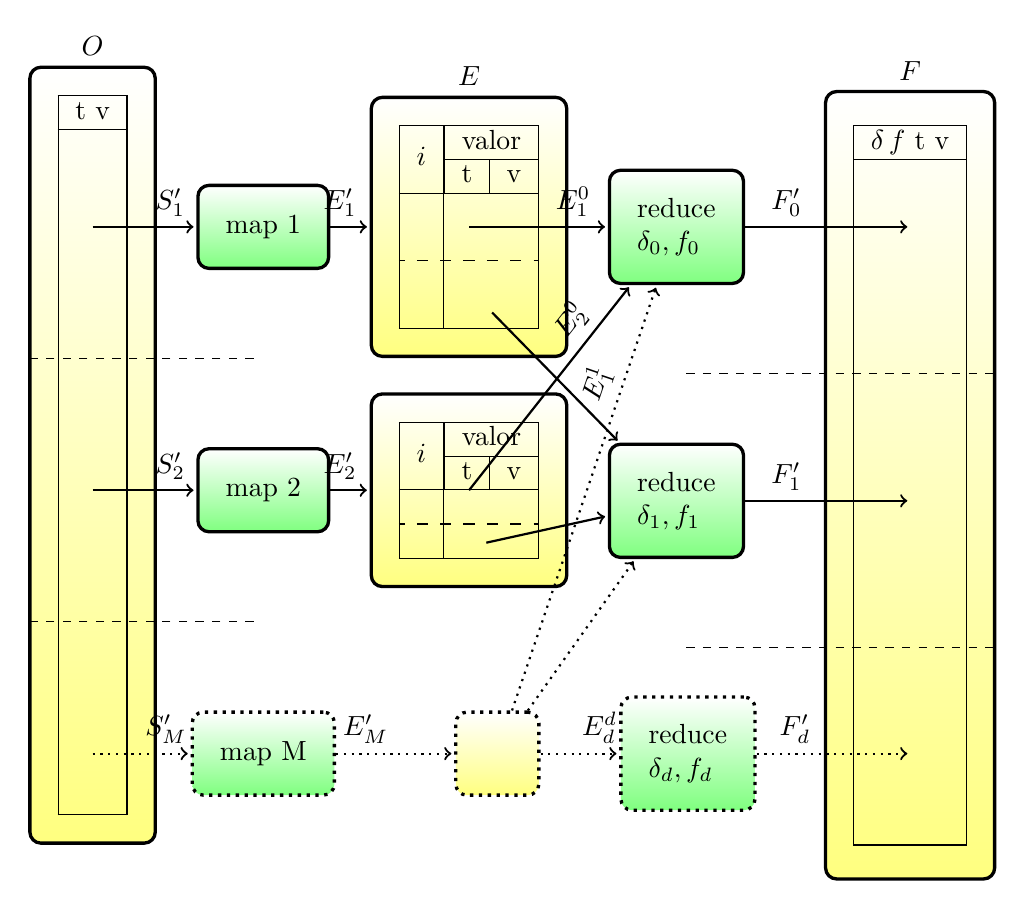
\begin{tikzpicture}

      \tikzset{
        mynode/.style={rectangle,rounded corners,draw=black, 
          very thick, inner sep=1em, minimum size=3em, text centered,
          groc},
        myarrow/.style={->, shorten >=1pt, thick},
        mylabel/.style={text width=7em, text centered},
        groc/.style={top color=white, bottom color=yellow!50},
        verd/.style={top color=white, bottom color=green!50},
        roig/.style={top color=white, bottom color=red!50},
      }  




 \node[mynode,verd] (m1) {map 1};
 \node (ml1) [below=of m1] {};
 \node[mynode,verd] (m2) [below=of ml1] {map 2};
 \node (ml2) [below=of m2] {};
 \node[mynode,verd,dotted] (mn) [below=of ml2] {map M};


 \node[mynode] (d1) [right=0.5cm of m1] {
   \begin{tabular}{|c|cc|}\hline
     \multirow{2}{*}{$i$} & \multicolumn{2}{|c|}{valor} \\\cline{2-3}
       & \multicolumn{1}{|c|}{t} & v \\\hline
      & & \\
      & &\\\hdashline
      & &\\
      & &\\\hline
   \end{tabular}
 };

 \node[mynode] (d2) [right=0.5cm of m2] {
   \begin{tabular}{|c|cc|}\hline
     \multirow{2}{*}{$i$} & \multicolumn{2}{|c|}{valor} \\\cline{2-3}
       & \multicolumn{1}{|c|}{t} & v \\\hline
      & &\\\hdashline
      & &\\\hline
   \end{tabular}
 };

 \node[mynode,dotted] (dn) [right=1.5cm of mn] {};



 \node[mynode,verd] (r1) [right=0.5cm of d1] {\parbox{1cm}{reduce $\delta_0,f_0$}};
 \node[mynode,verd] (r2) [below=2cm of r1] {\parbox{1cm}{reduce $\delta_1,f_1$}};
 \node[mynode,verd,dotted] (rn) [right=1cm of dn] {\parbox{1cm}{reduce $\delta_d,f_d$}};




 \node[mynode] (o) [above left=1.5cm and 0.5cm of m1, anchor=north east] {
   \begin{tabular}{|c|}\hline
     t v \\\hline
       \\
       \\
     \parbox[c][7cm][s]{0cm}{\vfill} \\
       \\
       \\\hline
   \end{tabular}
 };
 \node [above=0cm of o] {$O$};
 \node[mynode,minimum height=10cm] (f) [above right=of r1, anchor=north west] {
   \begin{tabular}{|c|}\hline
    $\delta\, f$ t v \\\hline
       \\
        \\
     \parbox[c][7cm][s]{0cm}{\vfill}  \\
        \\
        \\\hline
   \end{tabular}
};
 \node [above=0cm of f] {$F$};
 \node [above=0cm of d1] {$E$};




 \draw[dashed] (ml1) -- (ml1-|o.west);
 \draw[dashed] (ml2) -- (ml2-|o.west);

 \draw[myarrow] (o.center|-m1) -- (m1)  node[sloped,above,near end] {$S'_1$};
 \draw[myarrow] (o.center|-m2) -- (m2) node[sloped,above,near end] {$S'_2$};
 \draw[myarrow,dotted] (o.center|-mn) -- (mn) node[sloped,above,near end] {$S'_M$};


 \draw[myarrow] (m1) -- (d1) node[sloped,above,near start] {$E'_1$};
 \draw[myarrow] (m2) -- (d2) node[sloped,above,near start] {$E'_2$};
 \draw[myarrow,dotted] (mn) -- (dn)  node[sloped,above,near start] {$E'_M$};

 \draw[myarrow] (d1.center) -- (r1) node[sloped,above,near end] {$E_{1}^0$};
 \node (d1b) [above=3ex of d1.280] {}; 
 \draw[myarrow] (d1b.center) -- (r2) ;

 \draw[myarrow] (d2.center) -- (r1) node[sloped,above,near end] {$E_{2}^0$};
 \node (d2b) [above=3ex of d2.280] {}; 
 \draw[myarrow] (d2b.center) -- (r2) ;

 \draw[myarrow,dotted] (dn) -- (r1) node[sloped,above,near end] {$E_{1}^1$};
 \draw[myarrow,dotted] (dn) -- (r2);
 \draw[myarrow,dotted] (dn) -- (rn) node[sloped,above,near end] {$E_{d}^d$};


 \node (r1l) [below=of r1] {};
 \draw[dashed] (r1l) -- (r1l-|f.east);
 \node (r2l) [below=of r2] {};
 \draw[dashed] (r2l) -- (r2l-|f.east);


 \draw[myarrow] (r1) -- (r1-|f.center)  node[sloped,above,near start] {$F'_0$};
 \draw[myarrow] (r2) -- (r2-|f.center)  node[sloped,above,near start] {$F'_1$};
 \draw[myarrow,dotted] (rn) -- (rn-|f.center)  node[sloped,above,near start] {$F'_d$};


  \end{tikzpicture}
  
  \caption{Esquema de funcionament de RoundRobindoop}
  \label{fig:roundrobindoop:esquema}
\end{figure}






Les dades originals són la sèrie temporal $S$ és a dir un conjunt de
parelles de temps i valor, a les quals anomenem mesures. Un sèrie
temporal es pot partir en trossos on cada tros és un subconjunt de
mesures, és a dir una subsèrie temporal. Per tant, cada operació map
rep una subsèrie temporal de l'original: $S'_1 =
\{m_0,\dotsc,m_{o1}\}, S'_2 = \{m_{o1+1},\dotsc,m_{o2}\}, \dotsc, S'_M
= \{\dotsc,m_{k}\}$ on $M$ són el nombre de maps i $o_1,o_2\in
\glssymbol{not:N}$, $o_1 < o_2 < k$.



Les dades d'entremig són les sèries temporals dels buffers, és a dir
les mesures pendents de consolidar per a cada subsèrie resolució.
Així doncs, les dades d'entremig vistes com a conjunt són un conjunt
de dades pendents de consolidar $E=\{ D_{0}, \dotsc, D_t\}$ on cada
dada pendent de consolidar és un tuple $D=(i,m)$ on $i=(\delta,f,t_b)$
funciona com a identificador i $m=(t,v)$ com a valor.  És a dir, que
classifica cada mesura $m$ a quines resolucions s'han de consolidar
identificades pel pas de consolidació $\delta$, per la funció
d'agregació d'atributs $f$ i pel temps resultant de consolidació
$t_b$. Per tant, cada operació map resulta en un subconjunt de les
dades d'entremig: $E'_1=\{ (\delta_0,f_0, t_{b0}^0, t_0,v_0),
(\delta_1,f_1, t_{b1}^0, t_0,v_0), \dotsc , (\delta_d,f_d, t_{bd}^0,
t_0,v_0), (\delta_0,f_0, t_{b0}^1, t_1,v_1), \dotsc, (\delta_d,f_d,
t_{bd}^{o1}, t_{o1},v_{o1}) \}$, i $E'_2$ i $E'_M$ de manera similar.
En total, les dades d'entremig tenen un cardinal de $|E|=t+1=|e||S|$
és a dir la quantitat de resolucions de l'esquema multiplicat per la
quantitat de mesures de la sèrie temporal original.


Un cop calculades, les dades d'entremig $E$ s'ordenen i
s'agrupen per identificadors $(\delta,f, t_b)$ idèntics.  Així s'obté
unes dades d'entremig ordenades, de les quals expressem a continuació
cada subconjunt de forma simplificada agrupant per $\delta$ i $f$
sense tenir en comte els $t_b$. Siguin $ t_b, t,v$ variables lliures,
cada subconjunt agrupat de $E$ té la forma:
% Del subconjunt $E'_1$ s'obtenen els subconjunts $O_0^0= \{  (\delta_0,f_0, t_{b0}^0, t,v) \in E'_1 \}, O_0^1= \{  (\delta_0,f_0, t_{b0}^1, t,v) \in E'_1 \},\dotsc,  O_0^d= \{  (\delta_0,f_0, t_{b0}^{r0}, t,v) \in E'_1 \}$
a partir del subconjunt $E'_1$ s'obtenen $E_1^0=\{ (\delta_0,f_0, t_b,
t,v) \in E'_1 \}, E_1^1=\{ (\delta_1,f_1, t_b, t,v) \in E'_1 \},
\dotsc, E_1^d=\{ (\delta_d,f_d, t_b, t,v) \in E'_1 \}$, i de manera
similar s'obtenen els subconjunts agrupats a partir de
$E'_2,\dotsc,E'_d$.  D'aquesta manera cada operació reduce rep, en la
forma simplificada, tots els tuples de $E$ amb el mateix $\delta$ i
$f$: per a $\delta_0$ i $f_0$ rep $E^0 = E_1^0 \cup E_2^0 \cup \dotsb
\cup E_d^0$, per a $\delta_1$ i $f_1$ rep $E^1$, etc.  Com hem dit,
hem expressat aquests conjunts de forma simplificada per a $\delta$ i
$f$ tot i a més hi ha un reduce per a cada $t_b$ diferent; a
continuació per a les dades finals ho expressem de totes dues maneres.



Les dades finals són les sèries temporals dels discs, és a dir les
mesures consolidades per a cada subsèrie resolució. Així doncs, les
dades finals vistes com a conjunt són un conjunt de dades consolidades
$F=\{ D'_{0}, \dotsc, D'_r\}$ on cada dada consolidada és un tuple
$D'=(\delta,f,m')$ que indica quina mesura $m'=(t_b,v')$ és i a quin
disc pertany identificat per $\delta$ i $f$.  Per tant, cada operació
reduce calcula un subconjunt de $F$: $F_0^0
=\{(\delta_0,f_0,t_{b0}^0,v_0^0)\}, F_0^1
=\{(\delta_0,f_0,t_{b0}^1,v_0^1)\}, \dotsc, F_0^{r0}
=\{(\delta_0,f_0,t_{b0}^{r0},v_0^{r0})\}, F_1^0= \dotsc, F_1^{r1}=
\dotsc, F_d^0= \dotsc, F_d^{rd}=
\{(\delta_d,f_d,t_{bd}^{rd},v_d^{rd})\}$ on el nombre de mesures
consolidades per cada disc és afitat als cardinals màxims, $r_0 +1
\leq k_0, r_1 +1 \leq k_1, \dotsc r_d +1 \leq k_d$, i per tant el
nombre total de reduces està afitat a $|F| \leq k_0+k_1\dotsb+k_d$.
Per a simplificar la~\autoref{fig:roundrobindoop:esquema} s'han
agrupat els reduce per $\delta$ i $f$, és a dir $F'_0 =
\{(\delta_0,f_0,t_{b0}^0,v_0^0),(\delta_0,f_0,t_{b0}^1,v_0^1),\dotsc,
(\delta_0,f_0,t_{b0}^{r0},v_0^{r0})\}$, etc.\ i per tant $d+1= |e|$
són el nombre total de reduces agrupats.



L'operació map calcula les dades d'entremig a partir de les dades
originals i un esquema multiresolució, treballa en subconjunts de les
dades per a així poder-se computar para\l.lelament.
\begin{definition}[Operació Map]
  Sigui $S'=\{m_0,\dotsc,m_{o1}\}$ una subsèrie temporal de les dades
  originals, $e=\{ (\delta_0,f_0,\tau_0,k_0),\ldots,
  (\delta_d,f_d,\tau_d,k_d)\}$ un esquema de multiresolució i
  $E'=\{(\delta_0,f_0, t_{b0}^0, t_0,v_0),\dotsc, \dotsc,
  (\delta_d,f_d, t_{bd}^{o1}, t_{o1},v_{o1}) \}$ un subconjunt de les
  dades d'entremig abans de ser ordenades, l'operació map de
  l'algoritme MapReduce és $E'=\operatorname{map}(S',e)$ on $E'=
  \forall m \in S': \bigcup\operatorname{classifica}(m,e)$.

  La funció $\operatorname{classifica}$ indica per a cada mesura a quins
  discs s'ha de consolidar: $\operatorname{classifica}(m,e)=\{ \forall
  (\delta,f,\tau,k) \in e: (\delta,f,\tau+n\delta,t,v) |
  \tau+(n-1)\delta < t \leq \tau+n\delta, n\in\glssymbol{not:Z}, t >
  \tau \}$. Cal tenir en compte que $t > \tau$ indica que $\tau$ és el temps
  d'inici de la resolució i per tant no té sentit incloure mesures
  anteriors.
\end{definition}






Hi ha dues restriccions a la funció $\operatorname{classifica}$ que
hem definit: 
\begin{itemize}

\item S'assumeix que la $f$ treballa sobre l'interval de la sèrie
  original $S(\tau+(n-1)\delta ,\tau+n\delta]$. En cas que no sigui
  així per a la $f$ escollida, caldria modificar aquests intervals de
  classificació. A continuació d'aquest apartat contextualitzem aquest
  problema de les $f$.

\item No es tenen en compte els cardinals màxims. Si es volen tenir en
  compte, cal adequar bé els $\tau$ inicials. Així sigui $e$ l'esquema
  de multiresolució original, per a tenir en compte els cardinals
  màxims s'haurà d'usar un nou esquema $e'$ en què cada $\tau$
  original sigui canviat a un altre temps de consolidació múltiple
  $\tau'= \tau+n\delta$ (1) on $n\in\glssymbol{not:Z}$.  \emph{Càlcul
    de $n$:} es coneix $t_k=T(\max(S))$ i per a tenir en compte els
  cardinals s'ha de complir que $\tau'+k\delta \leq t_k$ (2), és a dir
  que les mesures entre $[\tau'+k\delta,t_k]$ encara no es poden
  consolidar.  Substituint la (1) a la (2) $\tau+n\delta+k\delta \leq
  t_k$, operant $\tau+(n+k)\delta \leq t_k$ i $n \leq
  \frac{t_k-\tau}{\delta}-k$ d'on es conclou que $n = \left\lfloor
    \frac{t_k-\tau}{\delta}-k \right\rfloor$ .  A més a més, si no es
  considera vàlid $\tau'<\tau$, és a dir que no es volen mesures abans
  del temps d'inici original, aleshores $n$ com a mínim pot valdre
  zero.

\end{itemize}



\begin{example}[Classificació d'una mesura en les resolucions]
  Sigui l'esquema de multiresolució
  $e=\{(\delta_0=2,f_0,\tau_0=0,k_0=4),(\delta_1=5,f_1,\tau_1=10,k_1=3)\}$
  i la mesura $m=(25,1)$, aquesta és classificada per a consolidar-se
  en les dues resolucions $\operatorname{classifica}(m,e)=\{
  (2,f_0,t_{b0},25,1), (5,f_1,t_{b1},25,1) \}$ on
  $\tau_0+(n-1)\delta_0 < 25 \leq \tau_0+n\delta_0,
  n\in\glssymbol{not:Z}$ i $t_{b0}=\tau_0+n\delta_0 = 26$, i de manera
  semblant $t_{b1}= 25$.

  Ara es volen tenir en compte els cardinals màxims, sigui
  $t_k=T(\max(S))=35$ el temps de la mesura màxima de la sèrie
  temporal original. Aleshores cal canviar l'esquema de multiresolució
  $e'=\{(\delta_0=2,f_0,\tau'_0,k_0=4),(\delta_1=5,f_1,\tau'_1,k_1=3)\}$
  on $\tau'_0=26$ i $\tau'_1=20$. La classificació esdevé
  $\operatorname{classifica}(m,e')=\{ (5,f_1,25,25,1) \}$ on no hi ha
  la resolució $\delta_0,f_0$ perquè $25< \tau'_0$.
\end{example}





Un cop s'han obtingut les dades d'entremig $E$, el sistema com per
exemple Hadoop agrupa els tuples de $E$ amb el mateix identificador i
els processa a un mateix reduce. És a dir, sigui $E$ la unió de tots
els $E'$ calculats pels map, un subconjunt de les dades ordenades és
$E''_{\delta,f,t_b} = \{ (\delta,f,t_b,m) \in E \}$.  L'operació
reduce calcula les dades finals a partir de les dades d'entremig
ordenades, treballa en subconjunts de les dades per a així poder-se
computar para\l.lelament.
\begin{definition}[Operació Reduce]
  Sigui $E''= \{ (\delta,f,t_b,m_0) ,\dotsc, (\delta,f,t_b,m_k) \}$ un
  subconjunt de les dades d'entremig ordenades i $F'=\{
  (\delta,f,t_b,v) \}$ un subconjunt de les dades finals, l'operació
  reduce de l'algoritme MapReduce és $F'=\operatorname{reduce}(E'')$
  on $F'= (\delta,f,t_b,v)$ i $v= V( f(\{m_0,\dotsc,m_k\},i))$ i
  $i=[t_b-\delta,t_b]$.
\end{definition}

L'expressió de l'interval $i$ es pot ometre ja que l'operació map ja
ha classificat les mesures d'aquest interval, tot i així l'indiquem
per a seguir la forma genèrica $f(S,i)$ de les funcions d'agregació
d'atributs de la definició. A continuació d'aquest apartat
contextualitzem aquest problema de les $f$.


En conclusió, el map i el reduce no es corresponen exactament
amb les definicions de les funcions de $\glssymbol{not:sgstm:dmap}$ i
$\glssymbol{not:sgstm:multiresolucio}$ \todo{ref a la secció?}, sinó
que el map classifica les mesures de la sèrie temporal segons el
buffer que els correspon i el reduce calcula les mesures consolidades
per un disc. És a dir, que un map i un reduce equivalen a la
funcionalitat de la funció $\glssymbol{not:sgstm:dmap}$ però el
conjunt de tots els maps i reduces equivalen a la funció de
$\glssymbol{not:sgstm:multiresolucio}$, sense expressar-ho en forma de
sèrie temporal total.



\subsubsection{Quant a les $f$ a RoundRobindoop}
\label{sec:mapreduce:f}

Al model de \gls{SGSTM} hem definit de forma genèrica les funcions
d'agregació d'atributs com a $m=f(S,i)$ (v. def.\todo{ref}). Aquestes funcions
principalment realitzen dues operacions: una selecció sobre la sèrie
temporal i una agregació de les mesures seleccionades. 

A RoundRobindoop, l'operació de selecció es duu a terme a l'etapa de
map i en canvi l'agregació, a l'etapa de reduce.  En l'algoritme de
MapReduce definit per a RoundRobindoop usem el model de $f$ descrit
anteriorment, però per a implementar correctament aquestes funcions
cal interpretar-ne el significat per a l'etapa de map i per a la de
reduce. És a dir, cada $f$ hauria de tenir dos components: un amb les
operacions de selecció per a ser usades en els map i l'altre amb les
operacions d'agregació per als reduce.


Així doncs, caldria afegir en els paràmetres de RoundRobindoop
l'operació de selecció d'interval per a cada $f$ que s'utilitzi. Però
això complica la resolució de l'algoritme de MapReduce. Per exemple,
resoldre l'interval temporal \gls{zohe}
--$S[t_0,t_f]^{\glssymbol{not:zohe}} = S(t_0,t_f] \cup \{
(t_f,V(\inf(S[t_f,+\infty))) \}$ (v.~def.\todo{ref a la def})--
implica conèixer la mesura següent a un $t_f$ i per tant treballar
sobre tota la sèrie temporal original, cosa que no és possible perquè
en les etapes map només es treballa sobre un subconjunt de la sèrie
temporal original. Això no obstant, per al RoundRobindoop definit, si
considerem que la sèrie temporal no té inframostreig aleshores en l'etapa
map podem fer la selecció prèvia per l'interval
$S(t_b-\delta,t_b+\delta]$, és a dir assumim que hi ha mesura a
$[t_b,t_b+\delta]$, i a l'etapa reduce ja es calcularà correctament
$f(S,[t_b-\delta,t_b])$. 


Recordem que en l'algoritme de RoundRobindoop definit hem assumit que
l'interval de selecció en l'etapa map sempre és $(t_b-\delta,t_b]$ i
en l'etapa reduce usem el model genèric d'agregació $f(S,i)$ tot i que
les mesures ja han estat seleccionades. Per tant, la interpretació en
l'etapa map no és vàlida per a totes les $f$.

Per tal d'ampliar l'etapa map, proposem una nova funció de
classificació que admeti ampliar l'interval de selecció. Si en la
classificació definida cada mesura es classificava en un i només un
$t_b$ per a cada resolució, en la nova funció de classificació es pot
escollir a quants $t_b$ es classifica cada mesura.  Sigui
$\operatorname{classifica}(m,e)$ la funció de classificació original i
sigui $l,g\in\glssymbol{not:N}$ les quantitats desitjades, la nova funció
de classificació és $\operatorname{classifica}'(m,e,l,g)=\{ \forall
(\delta,f,\tau,k) \in e: (\delta,f,\tau+(n-G_g)\delta,t,v), \dotsc,
(\delta,f,\tau+(n-G_0)\delta,t,v), (\delta,f,\tau+n\delta,t,v),
(\delta,f,\tau+(n+L_0)\delta,t,v), \dotsc,
(\delta,f,\tau+(n+L_l)\delta,t,v) | \tau+(n-1)\delta < t \leq
\tau+n\delta, n\in\glssymbol{not:Z}, t > \tau \}$ on
$L=\{1,2,\dotsc,l\}$ i $G=\{1,2,\dotsc,g\}$. El paràmetre $l$
permet classificar una mesura en temps posteriors i el paràmetre $g$
en temps anteriors; si ho observem des del punt de vista de la
selecció d'interval $S(t_b-(l+1)\delta,t_b+g\delta]$, el paràmetre $l$
permet estendre l'interval cap a l'esquerra i $g$ cap a la dreta.

\begin{example}[Classificació d'una mesura per \gls{zohe}]
  \label{ex:mapreduce:fzohe} 
  Com ja hem comentat, per a les funcions d'agregació d'atributs de la
  família \gls{zohe} s'ha d'aproximar l'interval temporal \gls{zohe} a
  una selecció en l'interval $S(t_b-\delta,t_b+\delta]$. És a dir, que
  la funció de classifica ha de retornar dues classificacions per a
  cada mesura, una amb $t_b$ i l'altra amb $t_b-\delta$. Per tant, per
  aquesta família $g=1$ i $l=0$.

  Sigui l'esquema de multiresolució
  $e=\{(\delta_0=2,f_0,\tau_0=0,k_0=4),(\delta_1=5,f_1,\tau_1=10,k_1=3)\}$
  i la mesura $m=(25,1)$, aquesta és classificada per a consolidar-se
  en les dues resolucions i en els dos instants per a cada un:
  $\operatorname{classifica}'(m,e,l=0,g=1)=\{
  (2,f_0,t_{b0}-g\delta_0,25,1), (2,f_0,t_{b0},25,1),
  (5,f_1,t_{b1}-g\delta_1,25,1), (5,f_1,t_{b1},25,1) \}$ on $t_{b0}=
  26$, $t_{b0}-g\delta_0= 24$, $t_{b1}= 25$ i $t_{b1}-g\delta_1= 20$.
  És a dir, es pot interpretar per a $\delta_0$ que quan es consolidi
  l'instant $24$ s'ha de fer la selecció $S(22,26]$ i per l'instant
  $26$ s'ha de fer la selecció $S(24,28]$, intervals en els quals hi
  ha la mesura $(25,1)$.

  A continuació, en l'apartat d'execució de l'algoritme, utilitzarem un exemple
  amb aquests processos de classificació.
\end{example}






En resum, el model de programació MapReduce limita les capacitats dels
\gls{SGSTM}, sobretot pel que fa a les funcions d'agregació
d'atributs. 






\subsection{Execució de l'algoritme}

\lstMakeShortInline[style=sh]{@}

Hadoop s'encarrega de l'execució de l'algoritme de MapReduce i de la
gestió de les dades d'entrada i de sortida.  Per a implementar-lo, cal
dissenyar un programa per al map i un programa per al reduce, els
quals reben de Hadoop els subconjunts de dades escaients i han de
retornar els subconjunts també escaients.  

Es pot utilitzar diferents llenguatges de programació a l'hora
d'implementar l'algoritme de MapReduce, hem escollit el llenguatge
Python \parencite{python:doc2}.  Implementem l'algoritme de MapReduce
que hem definit, RoundRobindoop, en un mateix programa que anomenem
@rrdoop.py@. El programa té un paràmetre que permet escollir l'etapa,
@rrdoop.py -map@ o @rrdoop.py -reduce@. A més també hi ha un paràmetre
per a definir l'esquema de multiresolució utilitzat, %
@rrdoop.py -map -schema e@.

El programa es comunica amb Hadoop mitjançant l'entrada estàndard
(stdin) per a rebre dades i mitjançant la sortida estàndard (stdout)
per a retornar els resultats.  Gràcies a la generalització del
programa amb comunicació per stdin i stdout, també es pot executar
l'algoritme de MapReduce al shell del sistema operatiu, cosa que
facilita l'experimentació amb l'algoritme.  Així, a continuació,
primer mostrem l'execució pas a pas de @rrdoop.py@ al shell i després
mostrem l'execució a Hadoop.



\subsubsection{Execució a la shell}

El~\autoref{lst:rrdoop:shell} és l'execució de
@rrdoop.py@ al shell del sistema operatiu. Només hi ha un procés map i
un procés reduce. Es comuniquen les dades a través de pipes (@|@) de la
shell i d'un procés d'ordenació (@sort@) que emula el procés
d'ordenació per identificador que faria Hadoop. A més, també s'emula
el procés de lectura (@cat@) de les dades originals.

\begin{lstlisting}[style=sh,caption=Execució a la shell de
  rrdoop.py,label=lst:rrdoop:shell]
cat original.csv | rrdoop.py -map -schema e.pickle -mapg 1 | sort -k1,1 | rrdoop.py -reduce -schema e.pickle  > final.csv
\end{lstlisting}


Les dades d'entrada són un fitxer, que també podrien ser fitxers de
dades, de les quals Hadoop en processa conjunts de línies a cada
procés map. Aquestes dades no cal que siguin ordenades i cal tenir en
compte que es poden trencar per qualsevol línia, tot i que Hadoop
permet configurar etapes que defineixin com s'han de partir els
fitxers.  Al~\autoref{lst:rrdoop:stdin} mostrem les dades d'entrada
emmagatzemades en el fitxer @original.csv@, que es corresponen
amb la sèrie temporal ja utilitzada
al~\autoref{lst:roundrobinson:ex1}.  Aquest fitxer de dades té format
de \gls{CSV}, com ja s'ha vist al~\autoref{lst:pytsms:storage} en les
funcionalitats complementàries per a l'emmagatzematge de Pytsms.
\begin{lstlisting}[style=file,caption=Dades d'entrada original.csv,label=lst:rrdoop:stdin]
1,6
8,5
5,2
10,0
14,1
19,6
26,6
29,0
22,11
\end{lstlisting}


El fitxer @original.csv@ es transmet a través de @cat@ i pipe a
l'stdin del procés de map %
@rrdoop.py -map -schema e.pickle -mapg 1@.  El procés de map té un esquema de
multiresolució com a paràmetre, @rrdoop.py@ a través del paràmetre
@-schema@ admet una sèrie temporal multiresolució en format Pickle,
com s'ha vist al~\autoref{lst:roundrobinson:storage}, l'esquema de la
qual serà el que s'utilitzi. En aquest cas, @e.pickle@ es correspon
amb el fitxer @mrd.pickle@ del~\autoref{lst:roundrobinson:storage} i
per tant amb l'esquema de multiresolució
del~\autoref{lst:roundrobinson:ex1}:
$e=\{(\delta_0=5,k_0=4,f_0=\glssymbol{not:sgstm:meanzohe},\tau_0=0),(\delta_1=10,k_1=2,f_1=\glssymbol{not:sgstm:maxzohe},\tau_1=0)\}$.


En aquest exemple d'esquema de multiresolució s'usen funcions
d'agregació d'atributs de la família \gls{zohe}. Com ja hem comentat a
l'\autoref{ex:mapreduce:fzohe}, s'ha de canviar la selecció que
l'etapa map duu a terme. A tal efecte RoundRobindoop admet un
paràmetre @-mapg@ per a indicar l'expansió de la classificació cap a
la dreta. Aproximem l'interval temporal \gls{zohe} a una selecció en
l'interval $(t_b-\delta,t_b+\delta]$, és a dir que hem d'expandir un
interval @-mapg 1@.  RoundRobindoop també admet un paràmetre @-mapl@
per a l'expansió cap a l'esquerra.


El procés de map retorna el resulta a través de l'stdout, el qual es
mostra al~\autoref{lst:rrdoop:sortidamap} i es correspon amb les dades
d'entremig de MapReduce. El format és el requerit per Hadoop, és a dir
cada línia és una parella d'identificador i valor separats per un
tabulador. L'identificador és $(\delta,\tau,t_b)$ però escrit en el
format $\delta$/$\tau$--$t_b$ i el valor és $(t,v)$ escrit separat per
un espai. Es pot observar com es comença classificant la primera
mesura $(1,6)$ en l'instant de consolidació $t_b=10$ per $\delta_1$ i
$t_b=5$ per $\delta_0$.  A continuació la mesura $(8,5)$ es classifica
a l'instant de consolidació $t_b=10$ per $\delta_1$ i en els $t_b=10$
i $t_b=5$ per $\delta_0$, en aquest darrer cas s'aplica l'aproximació
de la selecció \gls{zohe} per l'interval $(t_b-\delta,t_b+\delta]$;
cal destacar que en els casos anteriors no s'aplica perquè resultaria en
un $t_b<= \tau$.  I així per a totes fins a la darrera mesura
$(22,11)$.
\begin{lstlisting}[style=stdout,caption=Sortida del procés map,label=lst:rrdoop:sortidamap]
10/maximum_zohe-10	1 6.0
5/mean_zohe-5	1 6.0
10/maximum_zohe-10	8 5.0
5/mean_zohe-10	8 5.0
5/mean_zohe-5	8 5.0
10/maximum_zohe-10	5 2.0
5/mean_zohe-5	5 2.0
10/maximum_zohe-10	10 0.0
5/mean_zohe-10	10 0.0
5/mean_zohe-5	10 0.0
10/maximum_zohe-20	14 1.0
10/maximum_zohe-10	14 1.0
5/mean_zohe-15	14 1.0
5/mean_zohe-10	14 1.0
10/maximum_zohe-20	19 6.0
10/maximum_zohe-10	19 6.0
5/mean_zohe-20	19 6.0
5/mean_zohe-15	19 6.0
10/maximum_zohe-30	26 6.0
10/maximum_zohe-20	26 6.0
5/mean_zohe-30	26 6.0
5/mean_zohe-25	26 6.0
10/maximum_zohe-30	29 0.0
10/maximum_zohe-20	29 0.0
5/mean_zohe-30	29 0.0
5/mean_zohe-25	29 0.0
10/maximum_zohe-30	22 11.0
10/maximum_zohe-20	22 11.0
5/mean_zohe-25	22 11.0
5/mean_zohe-20	22 11.0
\end{lstlisting}


A continuació el procés d'ordenació @sort -k1,1@ ordena per
identificadors, el qual es mostra
al~\autoref{lst:rrdoop:sortidasort}. Hadoop agruparia els mateixos
identificadors i els transmetria a l'stdin d'un procés de reduce.
Observem per exemple la primera resolució @10/maximum_zohe-10@ que
conté les mesures en els instants de temps 10, 14, 1 ,19, 5 i 8;
l'agregació posterior haurà de treballar en l'interval \gls{zohe}
[0,10] i per tant ara queda clar que les mesures de 14 i 19 no són
necessàries, però això no ho podíem resoldre en l'etapa de map.
\begin{lstlisting}[style=stdout,caption=Sortida del procés d'ordenació,label=lst:rrdoop:sortidasort]
10/maximum_zohe-10	10 0.0
10/maximum_zohe-10	14 1.0
10/maximum_zohe-10	1 6.0
10/maximum_zohe-10	19 6.0
10/maximum_zohe-10	5 2.0
10/maximum_zohe-10	8 5.0
10/maximum_zohe-20	14 1.0
10/maximum_zohe-20	19 6.0
10/maximum_zohe-20	22 11.0
10/maximum_zohe-20	26 6.0
10/maximum_zohe-20	29 0.0
10/maximum_zohe-30	22 11.0
10/maximum_zohe-30	26 6.0
10/maximum_zohe-30	29 0.0
5/mean_zohe-10	10 0.0
5/mean_zohe-10	14 1.0
5/mean_zohe-10	8 5.0
5/mean_zohe-15	14 1.0
5/mean_zohe-15	19 6.0
5/mean_zohe-20	19 6.0
5/mean_zohe-20	22 11.0
5/mean_zohe-25	22 11.0
5/mean_zohe-25	26 6.0
5/mean_zohe-25	29 0.0
5/mean_zohe-30	26 6.0
5/mean_zohe-30	29 0.0
5/mean_zohe-5	10 0.0
5/mean_zohe-5	1 6.0
5/mean_zohe-5	5 2.0
5/mean_zohe-5	8 5.0
\end{lstlisting}


Finalment, el procés de reduce %
@rrdoop.py -reduce -schema e.pickle > final.csv@ obté de l'stdin les
dades del~\autoref{lst:rrdoop:sortidasort} i retorna les dades finals
per l'stdout que està redirigit al fitxer @final.csv@, el contingut
del qual es mostra al~\autoref{lst:rrdoop:sortidashell}.  Hadoop
emmagatzemaria aquestes dades en un fitxer o fitxers de dades.
Aquestes dades tenen el format $\delta$/$f$ $t_b$ $v$ on $(t_b,v)$ és
la mesura consolidada per a la resolució identificada per
$(\delta,f)$.

\begin{lstlisting}[style=file,caption=Dades de sortida final.csv,label=lst:rrdoop:sortidashell]
10/maximum_zohe	10 6.0
10/maximum_zohe	20 11.0
10/maximum_zohe	30 None
5/mean_zohe	10 3.0
5/mean_zohe	15 2.0
5/mean_zohe	20 7.0
5/mean_zohe	25 8.0
5/mean_zohe	30 None
5/mean_zohe	5 2.8
\end{lstlisting}

Així aquest resultat és el mateix que el de les consultes $\glssymbol{not:sgstm:seriedisc}(M,5,\glssymbol{not:sgstm:meanzohe})$ i $\glssymbol{not:sgstm:seriedisc}(M,10,\glssymbol{not:sgstm:maxzohe})$ del~\autoref{lst:roundrobinson:ex1} però amb les particularitats següents:

\begin{itemize}
\item RoundRobindoop no té en compte els cardinals màxims $k$ de les resolucions. Hi ha la mesura consolidada a l'instant $t_b=5$ per a la resolució $\delta_0=5$ que ja hauria d'haver estat eliminada per complir amb $k_0=4$.

\item RoundRobindoop no té en compte el temps màxim de la sèrie
  temporal original per a conèixer les mesures que encara no són
  consolidables. Hi ha la mesures en l'instant $t_b=30$ per a
  $\delta_0=5$ i $\delta_1=10$ que encara no podien ser calculades
  perquè $T(\max(S))=29$, de fet tenen valor nul (\emph{None}) a causa
  que l'interval \gls{zohe} no es pot calcular.

\item Així doncs, hi ha 9 mesures consolidades finals però 3 s'han de
  descartar. Per tant, per a la resolució $\delta_0=5$ hi ha 4 mesures
  i es compleix $4 \leq k_0=4$, i per a la resolució $\delta_1=10$ hi ha 2
  mesures i es compleix $2 \leq k_1=3$.
\end{itemize}




\subsubsection{Execució a Hadoop}


El~\autoref{lst:rrdoop:hadoop} mostra els passos d'execució de
@rrdoop.py@ a Hadoop. Primer cal copiar la sèrie temporal original a
\gls{HDFS}, després s'executa l'algoritme MapReduce i finalment es
recupera el resultat de \gls{HDFS}.  Hadoop streaming és l'eina que
permet l'execució a Hadoop de qualsevol programa, en qualsevol
llenguatge, que tingui el model de MapReduce.
Per a més detall sobre les ordres
i els processos vegeu la documentació de Hadoop~\parencite{hadoop}.
%http://hadoop.apache.org/docs/current/hadoop-mapreduce-client/hadoop-mapreduce-client-core/HadoopStreaming.html

\todo{simplificar alguns path, no cal tant detall aquí}

\begin{lstlisting}[style=sh,caption=Execució a Hadoop de
  rrdoop.py,label=lst:rrdoop:hadoop]
hadoop dfs -copyFromLocal original.csv /user/aleix/original.csv

hadoop jar /usr/lib/hadoop/contrib/streaming/hadoop-streaming*.jar -file rrdoop.py -file e.pickle  -mapper 'rrdoop.py -map -schema e.pickle -mapg 1' -reducer 'rrdoop.py -reduce -schema e.pickle' -input /user/aleix/original.csv -output /user/aleix/final

hadoop dfs -copyToLocal /user/aleix/final/part-00000 final.csv
\end{lstlisting}
%per esborrar: hadoop dfs -rmr /user/aleix/final
%requisit, tenir disponible roundrobinson, p.ex. cp -r ~/pfc_svn/src/roundrobinson/trunk/ /usr/local/lib/python2.7/dist-packages/roundrobinson

Per tal d'observar de manera senzilla l'execució de l'algoritme a
Hadoop hem realitzat una configuració anomenada \emph{Single Node
  Setup}, és a dir on només hi ha un computador que processa.  Un cop
verificat es podria estendre a una configuració de \emph{Cluster
  Setup}, en què hi hagués més computadors on distribuir les dades i
els processos.


El resultat és el mateix fitxer @final.csv@ que per a l'execució a la
shell, és a dir el~\autoref{lst:rrdoop:sortidashell}.  Hadoop gestiona
automàticament la distribució i la quantitat dels processos map i
reduce. Així, alguns dels map o reduces es poden ajuntar en el mateix
procés, per exemple els reduce poden rebre tant els subconjunts $E^0$
o $E''$ de la secció anterior, però mai se separa el mateix
identificador en diferents reduces. De fet, aquest és el cas quan
s'executa a la shell, on només hi ha un procés map i un de reduce.







% \subsubsection{Anàlisi de temps}


%Estaria bé comparar també amb pytsms, encara que s'ha de dir que no tenen res a veure perquè a pytsms no hem tingut gens en compte l'eficiència en el temps

% Per al temps s'hauria d'executar com a mínim 10 vegades cada experiment


% Analitzem el temps que triga en executar-se l'algoritme de MapReduce,
% tant en la shell com a Hadoop. En aquest darrer cas no incloem el
% temps de treballar amb el \gls{HDFS}.


% \begin{verbatim}
% * shell

% time cat matriu0.csv | ./rrdoop.py -map | sort -k1,1 | ./rrdoop.py -reduce > provant.csv::

%  real   0m21.639s
%  user   0m21.513s
%  sys    0m0.864s


% * hadoop

% time hadoop jar /usr/lib/hadoop/contrib/streaming/hadoop-streaming*.jar -file rrdoop.py -mapper 'rrdoop.py -map' -reducer 'rrdoop.py -reduce' -input /user/aleix/matriu0.csv -output /user/aleix/matriu::

%  real   0m28.314s
%  user   0m1.640s
%  sys    0m0.152s
% \end{verbatim}











\lstDeleteShortInline{@}



%%% Local Variables:
%%% TeX-master: "main"
%%% End:

  \caption{Esquema de funcionament de MapReduce}
  \label{fig:mapreduce:esquema}
\end{figure}



\begin{enumerate}

\item Hi ha unes dades originals que es poden partir en
  trossos. Hadoop està orientat a fitxers, mitjançant \gls{HDFS}, i
  per tant cada tros de dades és cadascun dels fitxers que es volen
  processar o bé conjunts de línies d'un fitxer.

\item Cada tros de les dades es processa mitjançant una operació
  map. Cada map es pot computar en para\l.lel i distribuït.

\item Cada operació map ha de retornar un nou conjunt de dades
  formats per parelles d'identificador i valor. Aquests conjunts de
  dades s'ordenen per identificador. 

\item Cada conjunt de dades amb el mateix identificador es processa
  mitjançant una operació reduce. Cada reduce es pot computar en
  para\l.lel i distribuït.

\item Cada reduce ha de retornar un tros del resultat final. És a dir,
  que unint les dades que retornen els reduce s'obtenen les dades
  finals. En l'orientació a fitxers de Hadoop, el resultat final és un
  fitxer, o bé un tros d'un fitxer, per a cada reduce.

\end{enumerate}



Per a resoldre un algoritme amb MapReduce, cal definir l'operació de
map i l'operació de reduce. El map ha de calcular un filtre sobre les
dades, sobretot establir grups de dades, i el reduce ha de calcular
agregacions o resums per a cada grup. MapReduce té una gran similitud
amb l'operació \emph{summarize} dels
\gls{SGBDR} \parencite[cap.~7]{date04:introduction8}, però separada
convenientment en les dues etapes.  A més, MapReduce imposa les
següents restriccions: les dades s'han de poder partir i l'algoritme
s'ha de poder expressar separat en les dues operacions de map i de
reduce.  \textcite{deanghemawat04:mapreduce} mostren exemples
d'algoritmes que es poden expressar amb MapReduce.



Un cop s'ha modelat un algoritme amb MapReduce, aleshores Hadoop ja és
capaç d'executar els maps i els reduces en para\l.lel i distribuïts. A
més, Hadoop també gestiona el compromís dels recursos entre el temps
de distribuir les dades, la quantitat de processos en para\l.lel que
s'han de crear i el temps afegit que suposa cada procés nou.








\section{RoundRobindoop}


RoundRobindoop implementa un \gls{SGSTM} específic que resol la funció
de multiresolució amb el model de programació MapReduce.  Per a
construir RoundRobindoop, primer dissenyem l'algoritme de MapReduce
que s'adequa a la multiresolució. Segon, proposem dues maneres per a
executar RoundRobindoop: amb Hadoop i la shell del sistema.



\subsection{Multiresolució amb MapReduce}

L'algoritme que implementem amb MapReduce és el de la funció de
multiresolució definida a la secció \todo{ref sec: multiresolucio: funcio}. Aquesta funció principalment té dues
parts, una de mapa i una de plec, que com ja s'ha dit no es poden
correspondre exactament amb les operacions de map i de reduce. 
 Així
doncs, dissenyem les operacions de map i de reduce que tenen el mateix
efecte que calcular la funció de multiresolució, en què el resultat
final no és la sèrie temporal total sinó el resultat de totes les
funcions $\glssymbol{not:sgstm:dmap}$, és a dir el resultat final són
les sèries temporals dels discs del model de \gls{SGSTM} la
concatenació dels quals resulta en la sèrie temporal total.



Sigui $S=\{m_0,m_1,\dotsc,m_k\}$ una sèrie temporal, i $e = \{
(\delta_0,f_0,\tau_0,k_0),\ldots, (\delta_d,f_d,\tau_d,k_d)\}$ els
paràmetres d'un esquema de multiresolució, definim l'algoritme
MapReduce que calcula $\operatorname{mapreduce}(S,e) = \{
(\delta_0,f_0,
\glssymbol{not:sgstm:dmap}(S,\delta_0,f_0,\tau_0,k_0)),\dotsc,
(\delta_c,f_c,\glssymbol{not:sgstm:dmap}(S,\delta_c,f_c,\tau_c,k_c))
\}$. És a dir, calcula tots els $\glssymbol{not:sgstm:dmap}$ possibles
i els identifica amb el pas de consolidació $\delta$ i la funció
d'agregació d'atributs $f$, els quals identifiquen les subsèries
resolució assumint que no n'hi ha de repetits.
%i que per tant tenenassociats el cardinal màxim $k$ i un instant de consolidació $\tau$.





L'esquema de funcionament de RoundRobindoop és el de
la~\autoref{fig:roundrobindoop:esquema}, el qual és la implementació
particular de l'esquema de la~\autoref{fig:mapreduce:esquema} per a la
multiresolució.  De forma resumida, RoundRobindoop en l'etapa de map
classifica les mesures en funció de a quin disc i temps resultant es
consolidaran i en l'etapa de reduce calcula la funció d'agregació per
a les mesures que s'hagin de consolidar al mateix disc.  A continuació
expliquem detalladament com són les dades originals ($O$), les
d'entremig ($E$) i les finals ($F$), i finalment definim l'operació de
map i la de reduce.





\begin{figure}[tp]
  \centering

  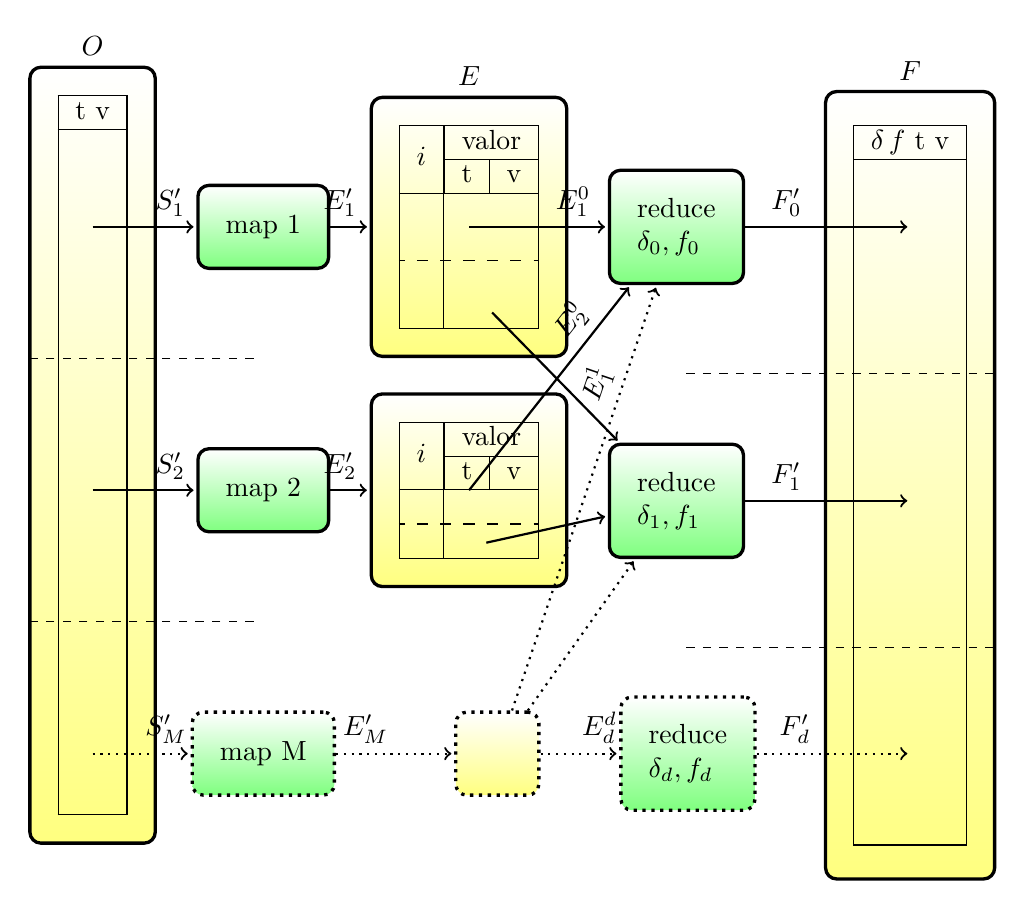
\begin{tikzpicture}

      \tikzset{
        mynode/.style={rectangle,rounded corners,draw=black, 
          very thick, inner sep=1em, minimum size=3em, text centered,
          groc},
        myarrow/.style={->, shorten >=1pt, thick},
        mylabel/.style={text width=7em, text centered},
        groc/.style={top color=white, bottom color=yellow!50},
        verd/.style={top color=white, bottom color=green!50},
        roig/.style={top color=white, bottom color=red!50},
      }  




 \node[mynode,verd] (m1) {map 1};
 \node (ml1) [below=of m1] {};
 \node[mynode,verd] (m2) [below=of ml1] {map 2};
 \node (ml2) [below=of m2] {};
 \node[mynode,verd,dotted] (mn) [below=of ml2] {map M};


 \node[mynode] (d1) [right=0.5cm of m1] {
   \begin{tabular}{|c|cc|}\hline
     \multirow{2}{*}{$i$} & \multicolumn{2}{|c|}{valor} \\\cline{2-3}
       & \multicolumn{1}{|c|}{t} & v \\\hline
      & & \\
      & &\\\hdashline
      & &\\
      & &\\\hline
   \end{tabular}
 };

 \node[mynode] (d2) [right=0.5cm of m2] {
   \begin{tabular}{|c|cc|}\hline
     \multirow{2}{*}{$i$} & \multicolumn{2}{|c|}{valor} \\\cline{2-3}
       & \multicolumn{1}{|c|}{t} & v \\\hline
      & &\\\hdashline
      & &\\\hline
   \end{tabular}
 };

 \node[mynode,dotted] (dn) [right=1.5cm of mn] {};



 \node[mynode,verd] (r1) [right=0.5cm of d1] {\parbox{1cm}{reduce $\delta_0,f_0$}};
 \node[mynode,verd] (r2) [below=2cm of r1] {\parbox{1cm}{reduce $\delta_1,f_1$}};
 \node[mynode,verd,dotted] (rn) [right=1cm of dn] {\parbox{1cm}{reduce $\delta_d,f_d$}};




 \node[mynode] (o) [above left=1.5cm and 0.5cm of m1, anchor=north east] {
   \begin{tabular}{|c|}\hline
     t v \\\hline
       \\
       \\
     \parbox[c][7cm][s]{0cm}{\vfill} \\
       \\
       \\\hline
   \end{tabular}
 };
 \node [above=0cm of o] {$O$};
 \node[mynode,minimum height=10cm] (f) [above right=of r1, anchor=north west] {
   \begin{tabular}{|c|}\hline
    $\delta\, f$ t v \\\hline
       \\
        \\
     \parbox[c][7cm][s]{0cm}{\vfill}  \\
        \\
        \\\hline
   \end{tabular}
};
 \node [above=0cm of f] {$F$};
 \node [above=0cm of d1] {$E$};




 \draw[dashed] (ml1) -- (ml1-|o.west);
 \draw[dashed] (ml2) -- (ml2-|o.west);

 \draw[myarrow] (o.center|-m1) -- (m1)  node[sloped,above,near end] {$S'_1$};
 \draw[myarrow] (o.center|-m2) -- (m2) node[sloped,above,near end] {$S'_2$};
 \draw[myarrow,dotted] (o.center|-mn) -- (mn) node[sloped,above,near end] {$S'_M$};


 \draw[myarrow] (m1) -- (d1) node[sloped,above,near start] {$E'_1$};
 \draw[myarrow] (m2) -- (d2) node[sloped,above,near start] {$E'_2$};
 \draw[myarrow,dotted] (mn) -- (dn)  node[sloped,above,near start] {$E'_M$};

 \draw[myarrow] (d1.center) -- (r1) node[sloped,above,near end] {$E_{1}^0$};
 \node (d1b) [above=3ex of d1.280] {}; 
 \draw[myarrow] (d1b.center) -- (r2) ;

 \draw[myarrow] (d2.center) -- (r1) node[sloped,above,near end] {$E_{2}^0$};
 \node (d2b) [above=3ex of d2.280] {}; 
 \draw[myarrow] (d2b.center) -- (r2) ;

 \draw[myarrow,dotted] (dn) -- (r1) node[sloped,above,near end] {$E_{1}^1$};
 \draw[myarrow,dotted] (dn) -- (r2);
 \draw[myarrow,dotted] (dn) -- (rn) node[sloped,above,near end] {$E_{d}^d$};


 \node (r1l) [below=of r1] {};
 \draw[dashed] (r1l) -- (r1l-|f.east);
 \node (r2l) [below=of r2] {};
 \draw[dashed] (r2l) -- (r2l-|f.east);


 \draw[myarrow] (r1) -- (r1-|f.center)  node[sloped,above,near start] {$F'_0$};
 \draw[myarrow] (r2) -- (r2-|f.center)  node[sloped,above,near start] {$F'_1$};
 \draw[myarrow,dotted] (rn) -- (rn-|f.center)  node[sloped,above,near start] {$F'_d$};


  \end{tikzpicture}
  
  \caption{Esquema de funcionament de RoundRobindoop}
  \label{fig:roundrobindoop:esquema}
\end{figure}






Les dades originals són la sèrie temporal $S$ és a dir un conjunt de
parelles de temps i valor, a les quals anomenem mesures. Un sèrie
temporal es pot partir en trossos on cada tros és un subconjunt de
mesures, és a dir una subsèrie temporal. Per tant, cada operació map
rep una subsèrie temporal de l'original: $S'_1 =
\{m_0,\dotsc,m_{o1}\}, S'_2 = \{m_{o1+1},\dotsc,m_{o2}\}, \dotsc, S'_M
= \{\dotsc,m_{k}\}$ on $M$ són el nombre de maps i $o_1,o_2\in
\glssymbol{not:N}$, $o_1 < o_2 < k$.



Les dades d'entremig són les sèries temporals dels buffers, és a dir
les mesures pendents de consolidar per a cada subsèrie resolució.
Així doncs, les dades d'entremig vistes com a conjunt són un conjunt
de dades pendents de consolidar $E=\{ D_{0}, \dotsc, D_t\}$ on cada
dada pendent de consolidar és un tuple $D=(i,m)$ on $i=(\delta,f,t_b)$
funciona com a identificador i $m=(t,v)$ com a valor.  És a dir, que
classifica cada mesura $m$ a quines resolucions s'han de consolidar
identificades pel pas de consolidació $\delta$, per la funció
d'agregació d'atributs $f$ i pel temps resultant de consolidació
$t_b$. Per tant, cada operació map resulta en un subconjunt de les
dades d'entremig: $E'_1=\{ (\delta_0,f_0, t_{b0}^0, t_0,v_0),
(\delta_1,f_1, t_{b1}^0, t_0,v_0), \dotsc , (\delta_d,f_d, t_{bd}^0,
t_0,v_0), (\delta_0,f_0, t_{b0}^1, t_1,v_1), \dotsc, (\delta_d,f_d,
t_{bd}^{o1}, t_{o1},v_{o1}) \}$, i $E'_2$ i $E'_M$ de manera similar.
En total, les dades d'entremig tenen un cardinal de $|E|=t+1=|e||S|$
és a dir la quantitat de resolucions de l'esquema multiplicat per la
quantitat de mesures de la sèrie temporal original.


Un cop calculades, les dades d'entremig $E$ s'ordenen i
s'agrupen per identificadors $(\delta,f, t_b)$ idèntics.  Així s'obté
unes dades d'entremig ordenades, de les quals expressem a continuació
cada subconjunt de forma simplificada agrupant per $\delta$ i $f$
sense tenir en comte els $t_b$. Siguin $ t_b, t,v$ variables lliures,
cada subconjunt agrupat de $E$ té la forma:
% Del subconjunt $E'_1$ s'obtenen els subconjunts $O_0^0= \{  (\delta_0,f_0, t_{b0}^0, t,v) \in E'_1 \}, O_0^1= \{  (\delta_0,f_0, t_{b0}^1, t,v) \in E'_1 \},\dotsc,  O_0^d= \{  (\delta_0,f_0, t_{b0}^{r0}, t,v) \in E'_1 \}$
a partir del subconjunt $E'_1$ s'obtenen $E_1^0=\{ (\delta_0,f_0, t_b,
t,v) \in E'_1 \}, E_1^1=\{ (\delta_1,f_1, t_b, t,v) \in E'_1 \},
\dotsc, E_1^d=\{ (\delta_d,f_d, t_b, t,v) \in E'_1 \}$, i de manera
similar s'obtenen els subconjunts agrupats a partir de
$E'_2,\dotsc,E'_d$.  D'aquesta manera cada operació reduce rep, en la
forma simplificada, tots els tuples de $E$ amb el mateix $\delta$ i
$f$: per a $\delta_0$ i $f_0$ rep $E^0 = E_1^0 \cup E_2^0 \cup \dotsb
\cup E_d^0$, per a $\delta_1$ i $f_1$ rep $E^1$, etc.  Com hem dit,
hem expressat aquests conjunts de forma simplificada per a $\delta$ i
$f$ tot i a més hi ha un reduce per a cada $t_b$ diferent; a
continuació per a les dades finals ho expressem de totes dues maneres.



Les dades finals són les sèries temporals dels discs, és a dir les
mesures consolidades per a cada subsèrie resolució. Així doncs, les
dades finals vistes com a conjunt són un conjunt de dades consolidades
$F=\{ D'_{0}, \dotsc, D'_r\}$ on cada dada consolidada és un tuple
$D'=(\delta,f,m')$ que indica quina mesura $m'=(t_b,v')$ és i a quin
disc pertany identificat per $\delta$ i $f$.  Per tant, cada operació
reduce calcula un subconjunt de $F$: $F_0^0
=\{(\delta_0,f_0,t_{b0}^0,v_0^0)\}, F_0^1
=\{(\delta_0,f_0,t_{b0}^1,v_0^1)\}, \dotsc, F_0^{r0}
=\{(\delta_0,f_0,t_{b0}^{r0},v_0^{r0})\}, F_1^0= \dotsc, F_1^{r1}=
\dotsc, F_d^0= \dotsc, F_d^{rd}=
\{(\delta_d,f_d,t_{bd}^{rd},v_d^{rd})\}$ on el nombre de mesures
consolidades per cada disc és afitat als cardinals màxims, $r_0 +1
\leq k_0, r_1 +1 \leq k_1, \dotsc r_d +1 \leq k_d$, i per tant el
nombre total de reduces està afitat a $|F| \leq k_0+k_1\dotsb+k_d$.
Per a simplificar la~\autoref{fig:roundrobindoop:esquema} s'han
agrupat els reduce per $\delta$ i $f$, és a dir $F'_0 =
\{(\delta_0,f_0,t_{b0}^0,v_0^0),(\delta_0,f_0,t_{b0}^1,v_0^1),\dotsc,
(\delta_0,f_0,t_{b0}^{r0},v_0^{r0})\}$, etc.\ i per tant $d+1= |e|$
són el nombre total de reduces agrupats.



L'operació map calcula les dades d'entremig a partir de les dades
originals i un esquema multiresolució, treballa en subconjunts de les
dades per a així poder-se computar para\l.lelament.
\begin{definition}[Operació Map]
  Sigui $S'=\{m_0,\dotsc,m_{o1}\}$ una subsèrie temporal de les dades
  originals, $e=\{ (\delta_0,f_0,\tau_0,k_0),\ldots,
  (\delta_d,f_d,\tau_d,k_d)\}$ un esquema de multiresolució i
  $E'=\{(\delta_0,f_0, t_{b0}^0, t_0,v_0),\dotsc, \dotsc,
  (\delta_d,f_d, t_{bd}^{o1}, t_{o1},v_{o1}) \}$ un subconjunt de les
  dades d'entremig abans de ser ordenades, l'operació map de
  l'algoritme MapReduce és $E'=\operatorname{map}(S',e)$ on $E'=
  \forall m \in S': \bigcup\operatorname{classifica}(m,e)$.

  La funció $\operatorname{classifica}$ indica per a cada mesura a quins
  discs s'ha de consolidar: $\operatorname{classifica}(m,e)=\{ \forall
  (\delta,f,\tau,k) \in e: (\delta,f,\tau+n\delta,t,v) |
  \tau+(n-1)\delta < t \leq \tau+n\delta, n\in\glssymbol{not:Z}, t >
  \tau \}$. Cal tenir en compte que $t > \tau$ indica que $\tau$ és el temps
  d'inici de la resolució i per tant no té sentit incloure mesures
  anteriors.
\end{definition}






Hi ha dues restriccions a la funció $\operatorname{classifica}$ que
hem definit: 
\begin{itemize}

\item S'assumeix que la $f$ treballa sobre l'interval de la sèrie
  original $S(\tau+(n-1)\delta ,\tau+n\delta]$. En cas que no sigui
  així per a la $f$ escollida, caldria modificar aquests intervals de
  classificació. A continuació d'aquest apartat contextualitzem aquest
  problema de les $f$.

\item No es tenen en compte els cardinals màxims. Si es volen tenir en
  compte, cal adequar bé els $\tau$ inicials. Així sigui $e$ l'esquema
  de multiresolució original, per a tenir en compte els cardinals
  màxims s'haurà d'usar un nou esquema $e'$ en què cada $\tau$
  original sigui canviat a un altre temps de consolidació múltiple
  $\tau'= \tau+n\delta$ (1) on $n\in\glssymbol{not:Z}$.  \emph{Càlcul
    de $n$:} es coneix $t_k=T(\max(S))$ i per a tenir en compte els
  cardinals s'ha de complir que $\tau'+k\delta \leq t_k$ (2), és a dir
  que les mesures entre $[\tau'+k\delta,t_k]$ encara no es poden
  consolidar.  Substituint la (1) a la (2) $\tau+n\delta+k\delta \leq
  t_k$, operant $\tau+(n+k)\delta \leq t_k$ i $n \leq
  \frac{t_k-\tau}{\delta}-k$ d'on es conclou que $n = \left\lfloor
    \frac{t_k-\tau}{\delta}-k \right\rfloor$ .  A més a més, si no es
  considera vàlid $\tau'<\tau$, és a dir que no es volen mesures abans
  del temps d'inici original, aleshores $n$ com a mínim pot valdre
  zero.

\end{itemize}



\begin{example}[Classificació d'una mesura en les resolucions]
  Sigui l'esquema de multiresolució
  $e=\{(\delta_0=2,f_0,\tau_0=0,k_0=4),(\delta_1=5,f_1,\tau_1=10,k_1=3)\}$
  i la mesura $m=(25,1)$, aquesta és classificada per a consolidar-se
  en les dues resolucions $\operatorname{classifica}(m,e)=\{
  (2,f_0,t_{b0},25,1), (5,f_1,t_{b1},25,1) \}$ on
  $\tau_0+(n-1)\delta_0 < 25 \leq \tau_0+n\delta_0,
  n\in\glssymbol{not:Z}$ i $t_{b0}=\tau_0+n\delta_0 = 26$, i de manera
  semblant $t_{b1}= 25$.

  Ara es volen tenir en compte els cardinals màxims, sigui
  $t_k=T(\max(S))=35$ el temps de la mesura màxima de la sèrie
  temporal original. Aleshores cal canviar l'esquema de multiresolució
  $e'=\{(\delta_0=2,f_0,\tau'_0,k_0=4),(\delta_1=5,f_1,\tau'_1,k_1=3)\}$
  on $\tau'_0=26$ i $\tau'_1=20$. La classificació esdevé
  $\operatorname{classifica}(m,e')=\{ (5,f_1,25,25,1) \}$ on no hi ha
  la resolució $\delta_0,f_0$ perquè $25< \tau'_0$.
\end{example}





Un cop s'han obtingut les dades d'entremig $E$, el sistema com per
exemple Hadoop agrupa els tuples de $E$ amb el mateix identificador i
els processa a un mateix reduce. És a dir, sigui $E$ la unió de tots
els $E'$ calculats pels map, un subconjunt de les dades ordenades és
$E''_{\delta,f,t_b} = \{ (\delta,f,t_b,m) \in E \}$.  L'operació
reduce calcula les dades finals a partir de les dades d'entremig
ordenades, treballa en subconjunts de les dades per a així poder-se
computar para\l.lelament.
\begin{definition}[Operació Reduce]
  Sigui $E''= \{ (\delta,f,t_b,m_0) ,\dotsc, (\delta,f,t_b,m_k) \}$ un
  subconjunt de les dades d'entremig ordenades i $F'=\{
  (\delta,f,t_b,v) \}$ un subconjunt de les dades finals, l'operació
  reduce de l'algoritme MapReduce és $F'=\operatorname{reduce}(E'')$
  on $F'= (\delta,f,t_b,v)$ i $v= V( f(\{m_0,\dotsc,m_k\},i))$ i
  $i=[t_b-\delta,t_b]$.
\end{definition}

L'expressió de l'interval $i$ es pot ometre ja que l'operació map ja
ha classificat les mesures d'aquest interval, tot i així l'indiquem
per a seguir la forma genèrica $f(S,i)$ de les funcions d'agregació
d'atributs de la definició. A continuació d'aquest apartat
contextualitzem aquest problema de les $f$.


En conclusió, el map i el reduce no es corresponen exactament
amb les definicions de les funcions de $\glssymbol{not:sgstm:dmap}$ i
$\glssymbol{not:sgstm:multiresolucio}$ \todo{ref a la secció?}, sinó
que el map classifica les mesures de la sèrie temporal segons el
buffer que els correspon i el reduce calcula les mesures consolidades
per un disc. És a dir, que un map i un reduce equivalen a la
funcionalitat de la funció $\glssymbol{not:sgstm:dmap}$ però el
conjunt de tots els maps i reduces equivalen a la funció de
$\glssymbol{not:sgstm:multiresolucio}$, sense expressar-ho en forma de
sèrie temporal total.



\subsubsection{Quant a les $f$ a RoundRobindoop}
\label{sec:mapreduce:f}

Al model de \gls{SGSTM} hem definit de forma genèrica les funcions
d'agregació d'atributs com a $m=f(S,i)$ (v. def.\todo{ref}). Aquestes funcions
principalment realitzen dues operacions: una selecció sobre la sèrie
temporal i una agregació de les mesures seleccionades. 

A RoundRobindoop, l'operació de selecció es duu a terme a l'etapa de
map i en canvi l'agregació, a l'etapa de reduce.  En l'algoritme de
MapReduce definit per a RoundRobindoop usem el model de $f$ descrit
anteriorment, però per a implementar correctament aquestes funcions
cal interpretar-ne el significat per a l'etapa de map i per a la de
reduce. És a dir, cada $f$ hauria de tenir dos components: un amb les
operacions de selecció per a ser usades en els map i l'altre amb les
operacions d'agregació per als reduce.


Així doncs, caldria afegir en els paràmetres de RoundRobindoop
l'operació de selecció d'interval per a cada $f$ que s'utilitzi. Però
això complica la resolució de l'algoritme de MapReduce. Per exemple,
resoldre l'interval temporal \gls{zohe}
--$S[t_0,t_f]^{\glssymbol{not:zohe}} = S(t_0,t_f] \cup \{
(t_f,V(\inf(S[t_f,+\infty))) \}$ (v.~def.\todo{ref a la def})--
implica conèixer la mesura següent a un $t_f$ i per tant treballar
sobre tota la sèrie temporal original, cosa que no és possible perquè
en les etapes map només es treballa sobre un subconjunt de la sèrie
temporal original. Això no obstant, per al RoundRobindoop definit, si
considerem que la sèrie temporal no té inframostreig aleshores en l'etapa
map podem fer la selecció prèvia per l'interval
$S(t_b-\delta,t_b+\delta]$, és a dir assumim que hi ha mesura a
$[t_b,t_b+\delta]$, i a l'etapa reduce ja es calcularà correctament
$f(S,[t_b-\delta,t_b])$. 


Recordem que en l'algoritme de RoundRobindoop definit hem assumit que
l'interval de selecció en l'etapa map sempre és $(t_b-\delta,t_b]$ i
en l'etapa reduce usem el model genèric d'agregació $f(S,i)$ tot i que
les mesures ja han estat seleccionades. Per tant, la interpretació en
l'etapa map no és vàlida per a totes les $f$.

Per tal d'ampliar l'etapa map, proposem una nova funció de
classificació que admeti ampliar l'interval de selecció. Si en la
classificació definida cada mesura es classificava en un i només un
$t_b$ per a cada resolució, en la nova funció de classificació es pot
escollir a quants $t_b$ es classifica cada mesura.  Sigui
$\operatorname{classifica}(m,e)$ la funció de classificació original i
sigui $l,g\in\glssymbol{not:N}$ les quantitats desitjades, la nova funció
de classificació és $\operatorname{classifica}'(m,e,l,g)=\{ \forall
(\delta,f,\tau,k) \in e: (\delta,f,\tau+(n-G_g)\delta,t,v), \dotsc,
(\delta,f,\tau+(n-G_0)\delta,t,v), (\delta,f,\tau+n\delta,t,v),
(\delta,f,\tau+(n+L_0)\delta,t,v), \dotsc,
(\delta,f,\tau+(n+L_l)\delta,t,v) | \tau+(n-1)\delta < t \leq
\tau+n\delta, n\in\glssymbol{not:Z}, t > \tau \}$ on
$L=\{1,2,\dotsc,l\}$ i $G=\{1,2,\dotsc,g\}$. El paràmetre $l$
permet classificar una mesura en temps posteriors i el paràmetre $g$
en temps anteriors; si ho observem des del punt de vista de la
selecció d'interval $S(t_b-(l+1)\delta,t_b+g\delta]$, el paràmetre $l$
permet estendre l'interval cap a l'esquerra i $g$ cap a la dreta.

\begin{example}[Classificació d'una mesura per \gls{zohe}]
  \label{ex:mapreduce:fzohe} 
  Com ja hem comentat, per a les funcions d'agregació d'atributs de la
  família \gls{zohe} s'ha d'aproximar l'interval temporal \gls{zohe} a
  una selecció en l'interval $S(t_b-\delta,t_b+\delta]$. És a dir, que
  la funció de classifica ha de retornar dues classificacions per a
  cada mesura, una amb $t_b$ i l'altra amb $t_b-\delta$. Per tant, per
  aquesta família $g=1$ i $l=0$.

  Sigui l'esquema de multiresolució
  $e=\{(\delta_0=2,f_0,\tau_0=0,k_0=4),(\delta_1=5,f_1,\tau_1=10,k_1=3)\}$
  i la mesura $m=(25,1)$, aquesta és classificada per a consolidar-se
  en les dues resolucions i en els dos instants per a cada un:
  $\operatorname{classifica}'(m,e,l=0,g=1)=\{
  (2,f_0,t_{b0}-g\delta_0,25,1), (2,f_0,t_{b0},25,1),
  (5,f_1,t_{b1}-g\delta_1,25,1), (5,f_1,t_{b1},25,1) \}$ on $t_{b0}=
  26$, $t_{b0}-g\delta_0= 24$, $t_{b1}= 25$ i $t_{b1}-g\delta_1= 20$.
  És a dir, es pot interpretar per a $\delta_0$ que quan es consolidi
  l'instant $24$ s'ha de fer la selecció $S(22,26]$ i per l'instant
  $26$ s'ha de fer la selecció $S(24,28]$, intervals en els quals hi
  ha la mesura $(25,1)$.

  A continuació, en l'apartat d'execució de l'algoritme, utilitzarem un exemple
  amb aquests processos de classificació.
\end{example}






En resum, el model de programació MapReduce limita les capacitats dels
\gls{SGSTM}, sobretot pel que fa a les funcions d'agregació
d'atributs. 






\subsection{Execució de l'algoritme}

\lstMakeShortInline[style=sh]{@}

Hadoop s'encarrega de l'execució de l'algoritme de MapReduce i de la
gestió de les dades d'entrada i de sortida.  Per a implementar-lo, cal
dissenyar un programa per al map i un programa per al reduce, els
quals reben de Hadoop els subconjunts de dades escaients i han de
retornar els subconjunts també escaients.  

Es pot utilitzar diferents llenguatges de programació a l'hora
d'implementar l'algoritme de MapReduce, hem escollit el llenguatge
Python \parencite{python:doc2}.  Implementem l'algoritme de MapReduce
que hem definit, RoundRobindoop, en un mateix programa que anomenem
@rrdoop.py@. El programa té un paràmetre que permet escollir l'etapa,
@rrdoop.py -map@ o @rrdoop.py -reduce@. A més també hi ha un paràmetre
per a definir l'esquema de multiresolució utilitzat, %
@rrdoop.py -map -schema e@.

El programa es comunica amb Hadoop mitjançant l'entrada estàndard
(stdin) per a rebre dades i mitjançant la sortida estàndard (stdout)
per a retornar els resultats.  Gràcies a la generalització del
programa amb comunicació per stdin i stdout, també es pot executar
l'algoritme de MapReduce al shell del sistema operatiu, cosa que
facilita l'experimentació amb l'algoritme.  Així, a continuació,
primer mostrem l'execució pas a pas de @rrdoop.py@ al shell i després
mostrem l'execució a Hadoop.



\subsubsection{Execució a la shell}

El~\autoref{lst:rrdoop:shell} és l'execució de
@rrdoop.py@ al shell del sistema operatiu. Només hi ha un procés map i
un procés reduce. Es comuniquen les dades a través de pipes (@|@) de la
shell i d'un procés d'ordenació (@sort@) que emula el procés
d'ordenació per identificador que faria Hadoop. A més, també s'emula
el procés de lectura (@cat@) de les dades originals.

\begin{lstlisting}[style=sh,caption=Execució a la shell de
  rrdoop.py,label=lst:rrdoop:shell]
cat original.csv | rrdoop.py -map -schema e.pickle -mapg 1 | sort -k1,1 | rrdoop.py -reduce -schema e.pickle  > final.csv
\end{lstlisting}


Les dades d'entrada són un fitxer, que també podrien ser fitxers de
dades, de les quals Hadoop en processa conjunts de línies a cada
procés map. Aquestes dades no cal que siguin ordenades i cal tenir en
compte que es poden trencar per qualsevol línia, tot i que Hadoop
permet configurar etapes que defineixin com s'han de partir els
fitxers.  Al~\autoref{lst:rrdoop:stdin} mostrem les dades d'entrada
emmagatzemades en el fitxer @original.csv@, que es corresponen
amb la sèrie temporal ja utilitzada
al~\autoref{lst:roundrobinson:ex1}.  Aquest fitxer de dades té format
de \gls{CSV}, com ja s'ha vist al~\autoref{lst:pytsms:storage} en les
funcionalitats complementàries per a l'emmagatzematge de Pytsms.
\begin{lstlisting}[style=file,caption=Dades d'entrada original.csv,label=lst:rrdoop:stdin]
1,6
8,5
5,2
10,0
14,1
19,6
26,6
29,0
22,11
\end{lstlisting}


El fitxer @original.csv@ es transmet a través de @cat@ i pipe a
l'stdin del procés de map %
@rrdoop.py -map -schema e.pickle -mapg 1@.  El procés de map té un esquema de
multiresolució com a paràmetre, @rrdoop.py@ a través del paràmetre
@-schema@ admet una sèrie temporal multiresolució en format Pickle,
com s'ha vist al~\autoref{lst:roundrobinson:storage}, l'esquema de la
qual serà el que s'utilitzi. En aquest cas, @e.pickle@ es correspon
amb el fitxer @mrd.pickle@ del~\autoref{lst:roundrobinson:storage} i
per tant amb l'esquema de multiresolució
del~\autoref{lst:roundrobinson:ex1}:
$e=\{(\delta_0=5,k_0=4,f_0=\glssymbol{not:sgstm:meanzohe},\tau_0=0),(\delta_1=10,k_1=2,f_1=\glssymbol{not:sgstm:maxzohe},\tau_1=0)\}$.


En aquest exemple d'esquema de multiresolució s'usen funcions
d'agregació d'atributs de la família \gls{zohe}. Com ja hem comentat a
l'\autoref{ex:mapreduce:fzohe}, s'ha de canviar la selecció que
l'etapa map duu a terme. A tal efecte RoundRobindoop admet un
paràmetre @-mapg@ per a indicar l'expansió de la classificació cap a
la dreta. Aproximem l'interval temporal \gls{zohe} a una selecció en
l'interval $(t_b-\delta,t_b+\delta]$, és a dir que hem d'expandir un
interval @-mapg 1@.  RoundRobindoop també admet un paràmetre @-mapl@
per a l'expansió cap a l'esquerra.


El procés de map retorna el resulta a través de l'stdout, el qual es
mostra al~\autoref{lst:rrdoop:sortidamap} i es correspon amb les dades
d'entremig de MapReduce. El format és el requerit per Hadoop, és a dir
cada línia és una parella d'identificador i valor separats per un
tabulador. L'identificador és $(\delta,\tau,t_b)$ però escrit en el
format $\delta$/$\tau$--$t_b$ i el valor és $(t,v)$ escrit separat per
un espai. Es pot observar com es comença classificant la primera
mesura $(1,6)$ en l'instant de consolidació $t_b=10$ per $\delta_1$ i
$t_b=5$ per $\delta_0$.  A continuació la mesura $(8,5)$ es classifica
a l'instant de consolidació $t_b=10$ per $\delta_1$ i en els $t_b=10$
i $t_b=5$ per $\delta_0$, en aquest darrer cas s'aplica l'aproximació
de la selecció \gls{zohe} per l'interval $(t_b-\delta,t_b+\delta]$;
cal destacar que en els casos anteriors no s'aplica perquè resultaria en
un $t_b<= \tau$.  I així per a totes fins a la darrera mesura
$(22,11)$.
\begin{lstlisting}[style=stdout,caption=Sortida del procés map,label=lst:rrdoop:sortidamap]
10/maximum_zohe-10	1 6.0
5/mean_zohe-5	1 6.0
10/maximum_zohe-10	8 5.0
5/mean_zohe-10	8 5.0
5/mean_zohe-5	8 5.0
10/maximum_zohe-10	5 2.0
5/mean_zohe-5	5 2.0
10/maximum_zohe-10	10 0.0
5/mean_zohe-10	10 0.0
5/mean_zohe-5	10 0.0
10/maximum_zohe-20	14 1.0
10/maximum_zohe-10	14 1.0
5/mean_zohe-15	14 1.0
5/mean_zohe-10	14 1.0
10/maximum_zohe-20	19 6.0
10/maximum_zohe-10	19 6.0
5/mean_zohe-20	19 6.0
5/mean_zohe-15	19 6.0
10/maximum_zohe-30	26 6.0
10/maximum_zohe-20	26 6.0
5/mean_zohe-30	26 6.0
5/mean_zohe-25	26 6.0
10/maximum_zohe-30	29 0.0
10/maximum_zohe-20	29 0.0
5/mean_zohe-30	29 0.0
5/mean_zohe-25	29 0.0
10/maximum_zohe-30	22 11.0
10/maximum_zohe-20	22 11.0
5/mean_zohe-25	22 11.0
5/mean_zohe-20	22 11.0
\end{lstlisting}


A continuació el procés d'ordenació @sort -k1,1@ ordena per
identificadors, el qual es mostra
al~\autoref{lst:rrdoop:sortidasort}. Hadoop agruparia els mateixos
identificadors i els transmetria a l'stdin d'un procés de reduce.
Observem per exemple la primera resolució @10/maximum_zohe-10@ que
conté les mesures en els instants de temps 10, 14, 1 ,19, 5 i 8;
l'agregació posterior haurà de treballar en l'interval \gls{zohe}
[0,10] i per tant ara queda clar que les mesures de 14 i 19 no són
necessàries, però això no ho podíem resoldre en l'etapa de map.
\begin{lstlisting}[style=stdout,caption=Sortida del procés d'ordenació,label=lst:rrdoop:sortidasort]
10/maximum_zohe-10	10 0.0
10/maximum_zohe-10	14 1.0
10/maximum_zohe-10	1 6.0
10/maximum_zohe-10	19 6.0
10/maximum_zohe-10	5 2.0
10/maximum_zohe-10	8 5.0
10/maximum_zohe-20	14 1.0
10/maximum_zohe-20	19 6.0
10/maximum_zohe-20	22 11.0
10/maximum_zohe-20	26 6.0
10/maximum_zohe-20	29 0.0
10/maximum_zohe-30	22 11.0
10/maximum_zohe-30	26 6.0
10/maximum_zohe-30	29 0.0
5/mean_zohe-10	10 0.0
5/mean_zohe-10	14 1.0
5/mean_zohe-10	8 5.0
5/mean_zohe-15	14 1.0
5/mean_zohe-15	19 6.0
5/mean_zohe-20	19 6.0
5/mean_zohe-20	22 11.0
5/mean_zohe-25	22 11.0
5/mean_zohe-25	26 6.0
5/mean_zohe-25	29 0.0
5/mean_zohe-30	26 6.0
5/mean_zohe-30	29 0.0
5/mean_zohe-5	10 0.0
5/mean_zohe-5	1 6.0
5/mean_zohe-5	5 2.0
5/mean_zohe-5	8 5.0
\end{lstlisting}


Finalment, el procés de reduce %
@rrdoop.py -reduce -schema e.pickle > final.csv@ obté de l'stdin les
dades del~\autoref{lst:rrdoop:sortidasort} i retorna les dades finals
per l'stdout que està redirigit al fitxer @final.csv@, el contingut
del qual es mostra al~\autoref{lst:rrdoop:sortidashell}.  Hadoop
emmagatzemaria aquestes dades en un fitxer o fitxers de dades.
Aquestes dades tenen el format $\delta$/$f$ $t_b$ $v$ on $(t_b,v)$ és
la mesura consolidada per a la resolució identificada per
$(\delta,f)$.

\begin{lstlisting}[style=file,caption=Dades de sortida final.csv,label=lst:rrdoop:sortidashell]
10/maximum_zohe	10 6.0
10/maximum_zohe	20 11.0
10/maximum_zohe	30 None
5/mean_zohe	10 3.0
5/mean_zohe	15 2.0
5/mean_zohe	20 7.0
5/mean_zohe	25 8.0
5/mean_zohe	30 None
5/mean_zohe	5 2.8
\end{lstlisting}

Així aquest resultat és el mateix que el de les consultes $\glssymbol{not:sgstm:seriedisc}(M,5,\glssymbol{not:sgstm:meanzohe})$ i $\glssymbol{not:sgstm:seriedisc}(M,10,\glssymbol{not:sgstm:maxzohe})$ del~\autoref{lst:roundrobinson:ex1} però amb les particularitats següents:

\begin{itemize}
\item RoundRobindoop no té en compte els cardinals màxims $k$ de les resolucions. Hi ha la mesura consolidada a l'instant $t_b=5$ per a la resolució $\delta_0=5$ que ja hauria d'haver estat eliminada per complir amb $k_0=4$.

\item RoundRobindoop no té en compte el temps màxim de la sèrie
  temporal original per a conèixer les mesures que encara no són
  consolidables. Hi ha la mesures en l'instant $t_b=30$ per a
  $\delta_0=5$ i $\delta_1=10$ que encara no podien ser calculades
  perquè $T(\max(S))=29$, de fet tenen valor nul (\emph{None}) a causa
  que l'interval \gls{zohe} no es pot calcular.

\item Així doncs, hi ha 9 mesures consolidades finals però 3 s'han de
  descartar. Per tant, per a la resolució $\delta_0=5$ hi ha 4 mesures
  i es compleix $4 \leq k_0=4$, i per a la resolució $\delta_1=10$ hi ha 2
  mesures i es compleix $2 \leq k_1=3$.
\end{itemize}




\subsubsection{Execució a Hadoop}


El~\autoref{lst:rrdoop:hadoop} mostra els passos d'execució de
@rrdoop.py@ a Hadoop. Primer cal copiar la sèrie temporal original a
\gls{HDFS}, després s'executa l'algoritme MapReduce i finalment es
recupera el resultat de \gls{HDFS}.  Hadoop streaming és l'eina que
permet l'execució a Hadoop de qualsevol programa, en qualsevol
llenguatge, que tingui el model de MapReduce.
Per a més detall sobre les ordres
i els processos vegeu la documentació de Hadoop~\parencite{hadoop}.
%http://hadoop.apache.org/docs/current/hadoop-mapreduce-client/hadoop-mapreduce-client-core/HadoopStreaming.html

\todo{simplificar alguns path, no cal tant detall aquí}

\begin{lstlisting}[style=sh,caption=Execució a Hadoop de
  rrdoop.py,label=lst:rrdoop:hadoop]
hadoop dfs -copyFromLocal original.csv /user/aleix/original.csv

hadoop jar /usr/lib/hadoop/contrib/streaming/hadoop-streaming*.jar -file rrdoop.py -file e.pickle  -mapper 'rrdoop.py -map -schema e.pickle -mapg 1' -reducer 'rrdoop.py -reduce -schema e.pickle' -input /user/aleix/original.csv -output /user/aleix/final

hadoop dfs -copyToLocal /user/aleix/final/part-00000 final.csv
\end{lstlisting}
%per esborrar: hadoop dfs -rmr /user/aleix/final
%requisit, tenir disponible roundrobinson, p.ex. cp -r ~/pfc_svn/src/roundrobinson/trunk/ /usr/local/lib/python2.7/dist-packages/roundrobinson

Per tal d'observar de manera senzilla l'execució de l'algoritme a
Hadoop hem realitzat una configuració anomenada \emph{Single Node
  Setup}, és a dir on només hi ha un computador que processa.  Un cop
verificat es podria estendre a una configuració de \emph{Cluster
  Setup}, en què hi hagués més computadors on distribuir les dades i
els processos.


El resultat és el mateix fitxer @final.csv@ que per a l'execució a la
shell, és a dir el~\autoref{lst:rrdoop:sortidashell}.  Hadoop gestiona
automàticament la distribució i la quantitat dels processos map i
reduce. Així, alguns dels map o reduces es poden ajuntar en el mateix
procés, per exemple els reduce poden rebre tant els subconjunts $E^0$
o $E''$ de la secció anterior, però mai se separa el mateix
identificador en diferents reduces. De fet, aquest és el cas quan
s'executa a la shell, on només hi ha un procés map i un de reduce.







% \subsubsection{Anàlisi de temps}


%Estaria bé comparar també amb pytsms, encara que s'ha de dir que no tenen res a veure perquè a pytsms no hem tingut gens en compte l'eficiència en el temps

% Per al temps s'hauria d'executar com a mínim 10 vegades cada experiment


% Analitzem el temps que triga en executar-se l'algoritme de MapReduce,
% tant en la shell com a Hadoop. En aquest darrer cas no incloem el
% temps de treballar amb el \gls{HDFS}.


% \begin{verbatim}
% * shell

% time cat matriu0.csv | ./rrdoop.py -map | sort -k1,1 | ./rrdoop.py -reduce > provant.csv::

%  real   0m21.639s
%  user   0m21.513s
%  sys    0m0.864s


% * hadoop

% time hadoop jar /usr/lib/hadoop/contrib/streaming/hadoop-streaming*.jar -file rrdoop.py -mapper 'rrdoop.py -map' -reducer 'rrdoop.py -reduce' -input /user/aleix/matriu0.csv -output /user/aleix/matriu::

%  real   0m28.314s
%  user   0m1.640s
%  sys    0m0.152s
% \end{verbatim}











\lstDeleteShortInline{@}



%%% Local Variables:
%%% TeX-master: "main"
%%% End:

  \caption{Esquema de funcionament de MapReduce}
  \label{fig:mapreduce:esquema}
\end{figure}



\begin{enumerate}

\item Hi ha unes dades originals que es poden partir en
  trossos. Hadoop està orientat a fitxers, mitjançant \gls{HDFS}, i
  per tant cada tros de dades és cadascun dels fitxers que es volen
  processar o bé conjunts de línies d'un fitxer.

\item Cada tros de les dades es processa mitjançant una operació
  map. Cada map es pot computar en para\l.lel i distribuït.

\item Cada operació map ha de retornar un nou conjunt de dades
  formats per parelles d'identificador i valor. Aquests conjunts de
  dades s'ordenen per identificador. 

\item Cada conjunt de dades amb el mateix identificador es processa
  mitjançant una operació reduce. Cada reduce es pot computar en
  para\l.lel i distribuït.

\item Cada reduce ha de retornar un tros del resultat final. És a dir,
  que unint les dades que retornen els reduce s'obtenen les dades
  finals. En l'orientació a fitxers de Hadoop, el resultat final és un
  fitxer, o bé un tros d'un fitxer, per a cada reduce.

\end{enumerate}



Per a resoldre un algoritme amb MapReduce, cal definir l'operació de
map i l'operació de reduce. El map ha de calcular un filtre sobre les
dades, sobretot establir grups de dades, i el reduce ha de calcular
agregacions o resums per a cada grup. MapReduce té una gran similitud
amb l'operació \emph{summarize} dels
\gls{SGBDR} \parencite[cap.~7]{date04:introduction8}, però separada
convenientment en les dues etapes.  A més, MapReduce imposa les
següents restriccions: les dades s'han de poder partir i l'algoritme
s'ha de poder expressar separat en les dues operacions de map i de
reduce.  \textcite{deanghemawat04:mapreduce} mostren exemples
d'algoritmes que es poden expressar amb MapReduce.



Un cop s'ha modelat un algoritme amb MapReduce, aleshores Hadoop ja és
capaç d'executar els maps i els reduces en para\l.lel i distribuïts. A
més, Hadoop també gestiona el compromís dels recursos entre el temps
de distribuir les dades, la quantitat de processos en para\l.lel que
s'han de crear i el temps afegit que suposa cada procés nou.








\section{RoundRobindoop}


RoundRobindoop implementa un \gls{SGSTM} específic que resol la funció
de multiresolució amb el model de programació MapReduce.  Per a
construir RoundRobindoop, primer dissenyem l'algoritme de MapReduce
que s'adequa a la multiresolució. Segon, proposem dues maneres per a
executar RoundRobindoop: amb Hadoop i la shell del sistema.



\subsection{Multiresolució amb MapReduce}

L'algoritme que implementem amb MapReduce és el de la funció de
multiresolució definida a la secció \todo{ref sec: multiresolucio: funcio}. Aquesta funció principalment té dues
parts, una de mapa i una de plec, que com ja s'ha dit no es poden
correspondre exactament amb les operacions de map i de reduce. 
 Així
doncs, dissenyem les operacions de map i de reduce que tenen el mateix
efecte que calcular la funció de multiresolució, en què el resultat
final no és la sèrie temporal total sinó el resultat de totes les
funcions $\glssymbol{not:sgstm:dmap}$, és a dir el resultat final són
les sèries temporals dels discs del model de \gls{SGSTM} la
concatenació dels quals resulta en la sèrie temporal total.



Sigui $S=\{m_0,m_1,\dotsc,m_k\}$ una sèrie temporal, i $e = \{
(\delta_0,f_0,\tau_0,k_0),\ldots, (\delta_d,f_d,\tau_d,k_d)\}$ els
paràmetres d'un esquema de multiresolució, definim l'algoritme
MapReduce que calcula $\operatorname{mapreduce}(S,e) = \{
(\delta_0,f_0,
\glssymbol{not:sgstm:dmap}(S,\delta_0,f_0,\tau_0,k_0)),\dotsc,
(\delta_c,f_c,\glssymbol{not:sgstm:dmap}(S,\delta_c,f_c,\tau_c,k_c))
\}$. És a dir, calcula tots els $\glssymbol{not:sgstm:dmap}$ possibles
i els identifica amb el pas de consolidació $\delta$ i la funció
d'agregació d'atributs $f$, els quals identifiquen les subsèries
resolució assumint que no n'hi ha de repetits.
%i que per tant tenenassociats el cardinal màxim $k$ i un instant de consolidació $\tau$.





L'esquema de funcionament de RoundRobindoop és el de
la~\autoref{fig:roundrobindoop:esquema}, el qual és la implementació
particular de l'esquema de la~\autoref{fig:mapreduce:esquema} per a la
multiresolució.  De forma resumida, RoundRobindoop en l'etapa de map
classifica les mesures en funció de a quin disc i temps resultant es
consolidaran i en l'etapa de reduce calcula la funció d'agregació per
a les mesures que s'hagin de consolidar al mateix disc.  A continuació
expliquem detalladament com són les dades originals ($O$), les
d'entremig ($E$) i les finals ($F$), i finalment definim l'operació de
map i la de reduce.





\begin{figure}[tp]
  \centering

  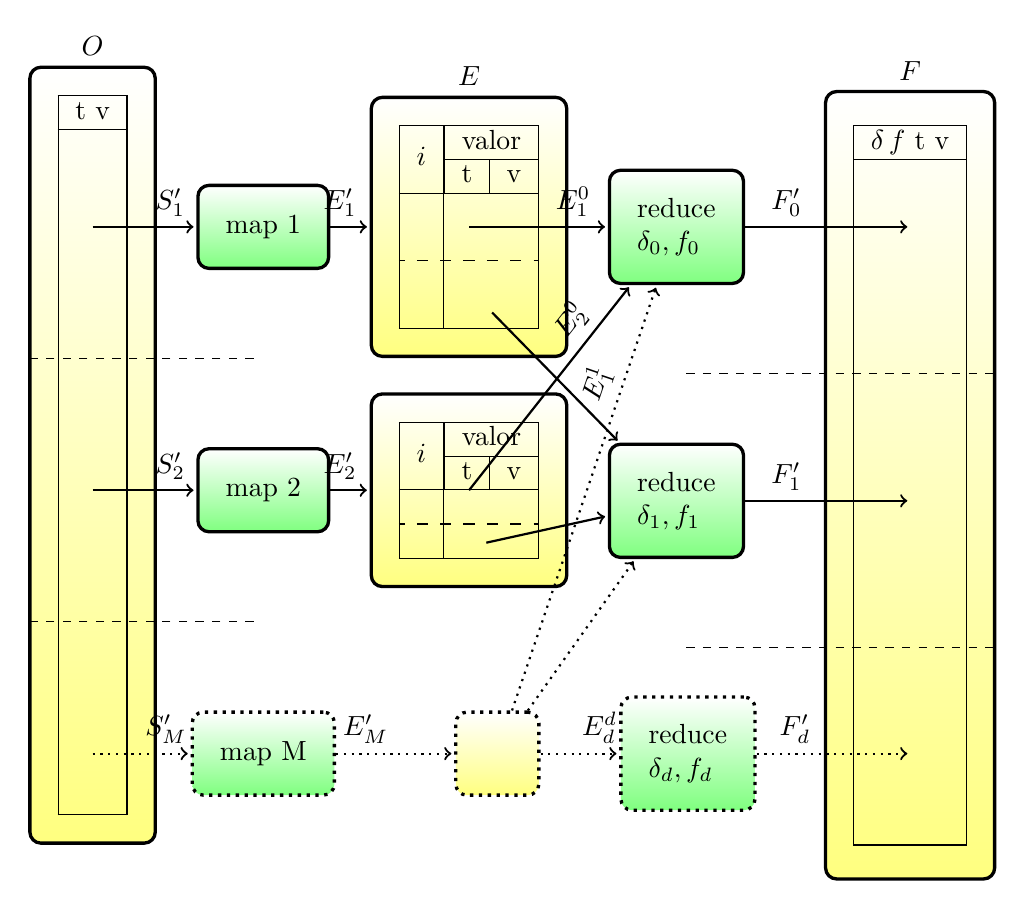
\begin{tikzpicture}

      \tikzset{
        mynode/.style={rectangle,rounded corners,draw=black, 
          very thick, inner sep=1em, minimum size=3em, text centered,
          groc},
        myarrow/.style={->, shorten >=1pt, thick},
        mylabel/.style={text width=7em, text centered},
        groc/.style={top color=white, bottom color=yellow!50},
        verd/.style={top color=white, bottom color=green!50},
        roig/.style={top color=white, bottom color=red!50},
      }  




 \node[mynode,verd] (m1) {map 1};
 \node (ml1) [below=of m1] {};
 \node[mynode,verd] (m2) [below=of ml1] {map 2};
 \node (ml2) [below=of m2] {};
 \node[mynode,verd,dotted] (mn) [below=of ml2] {map M};


 \node[mynode] (d1) [right=0.5cm of m1] {
   \begin{tabular}{|c|cc|}\hline
     \multirow{2}{*}{$i$} & \multicolumn{2}{|c|}{valor} \\\cline{2-3}
       & \multicolumn{1}{|c|}{t} & v \\\hline
      & & \\
      & &\\\hdashline
      & &\\
      & &\\\hline
   \end{tabular}
 };

 \node[mynode] (d2) [right=0.5cm of m2] {
   \begin{tabular}{|c|cc|}\hline
     \multirow{2}{*}{$i$} & \multicolumn{2}{|c|}{valor} \\\cline{2-3}
       & \multicolumn{1}{|c|}{t} & v \\\hline
      & &\\\hdashline
      & &\\\hline
   \end{tabular}
 };

 \node[mynode,dotted] (dn) [right=1.5cm of mn] {};



 \node[mynode,verd] (r1) [right=0.5cm of d1] {\parbox{1cm}{reduce $\delta_0,f_0$}};
 \node[mynode,verd] (r2) [below=2cm of r1] {\parbox{1cm}{reduce $\delta_1,f_1$}};
 \node[mynode,verd,dotted] (rn) [right=1cm of dn] {\parbox{1cm}{reduce $\delta_d,f_d$}};




 \node[mynode] (o) [above left=1.5cm and 0.5cm of m1, anchor=north east] {
   \begin{tabular}{|c|}\hline
     t v \\\hline
       \\
       \\
     \parbox[c][7cm][s]{0cm}{\vfill} \\
       \\
       \\\hline
   \end{tabular}
 };
 \node [above=0cm of o] {$O$};
 \node[mynode,minimum height=10cm] (f) [above right=of r1, anchor=north west] {
   \begin{tabular}{|c|}\hline
    $\delta\, f$ t v \\\hline
       \\
        \\
     \parbox[c][7cm][s]{0cm}{\vfill}  \\
        \\
        \\\hline
   \end{tabular}
};
 \node [above=0cm of f] {$F$};
 \node [above=0cm of d1] {$E$};




 \draw[dashed] (ml1) -- (ml1-|o.west);
 \draw[dashed] (ml2) -- (ml2-|o.west);

 \draw[myarrow] (o.center|-m1) -- (m1)  node[sloped,above,near end] {$S'_1$};
 \draw[myarrow] (o.center|-m2) -- (m2) node[sloped,above,near end] {$S'_2$};
 \draw[myarrow,dotted] (o.center|-mn) -- (mn) node[sloped,above,near end] {$S'_M$};


 \draw[myarrow] (m1) -- (d1) node[sloped,above,near start] {$E'_1$};
 \draw[myarrow] (m2) -- (d2) node[sloped,above,near start] {$E'_2$};
 \draw[myarrow,dotted] (mn) -- (dn)  node[sloped,above,near start] {$E'_M$};

 \draw[myarrow] (d1.center) -- (r1) node[sloped,above,near end] {$E_{1}^0$};
 \node (d1b) [above=3ex of d1.280] {}; 
 \draw[myarrow] (d1b.center) -- (r2) ;

 \draw[myarrow] (d2.center) -- (r1) node[sloped,above,near end] {$E_{2}^0$};
 \node (d2b) [above=3ex of d2.280] {}; 
 \draw[myarrow] (d2b.center) -- (r2) ;

 \draw[myarrow,dotted] (dn) -- (r1) node[sloped,above,near end] {$E_{1}^1$};
 \draw[myarrow,dotted] (dn) -- (r2);
 \draw[myarrow,dotted] (dn) -- (rn) node[sloped,above,near end] {$E_{d}^d$};


 \node (r1l) [below=of r1] {};
 \draw[dashed] (r1l) -- (r1l-|f.east);
 \node (r2l) [below=of r2] {};
 \draw[dashed] (r2l) -- (r2l-|f.east);


 \draw[myarrow] (r1) -- (r1-|f.center)  node[sloped,above,near start] {$F'_0$};
 \draw[myarrow] (r2) -- (r2-|f.center)  node[sloped,above,near start] {$F'_1$};
 \draw[myarrow,dotted] (rn) -- (rn-|f.center)  node[sloped,above,near start] {$F'_d$};


  \end{tikzpicture}
  
  \caption{Esquema de funcionament de RoundRobindoop}
  \label{fig:roundrobindoop:esquema}
\end{figure}






Les dades originals són la sèrie temporal $S$ és a dir un conjunt de
parelles de temps i valor, a les quals anomenem mesures. Un sèrie
temporal es pot partir en trossos on cada tros és un subconjunt de
mesures, és a dir una subsèrie temporal. Per tant, cada operació map
rep una subsèrie temporal de l'original: $S'_1 =
\{m_0,\dotsc,m_{o1}\}, S'_2 = \{m_{o1+1},\dotsc,m_{o2}\}, \dotsc, S'_M
= \{\dotsc,m_{k}\}$ on $M$ són el nombre de maps i $o_1,o_2\in
\glssymbol{not:N}$, $o_1 < o_2 < k$.



Les dades d'entremig són les sèries temporals dels buffers, és a dir
les mesures pendents de consolidar per a cada subsèrie resolució.
Així doncs, les dades d'entremig vistes com a conjunt són un conjunt
de dades pendents de consolidar $E=\{ D_{0}, \dotsc, D_t\}$ on cada
dada pendent de consolidar és un tuple $D=(i,m)$ on $i=(\delta,f,t_b)$
funciona com a identificador i $m=(t,v)$ com a valor.  És a dir, que
classifica cada mesura $m$ a quines resolucions s'han de consolidar
identificades pel pas de consolidació $\delta$, per la funció
d'agregació d'atributs $f$ i pel temps resultant de consolidació
$t_b$. Per tant, cada operació map resulta en un subconjunt de les
dades d'entremig: $E'_1=\{ (\delta_0,f_0, t_{b0}^0, t_0,v_0),
(\delta_1,f_1, t_{b1}^0, t_0,v_0), \dotsc , (\delta_d,f_d, t_{bd}^0,
t_0,v_0), (\delta_0,f_0, t_{b0}^1, t_1,v_1), \dotsc, (\delta_d,f_d,
t_{bd}^{o1}, t_{o1},v_{o1}) \}$, i $E'_2$ i $E'_M$ de manera similar.
En total, les dades d'entremig tenen un cardinal de $|E|=t+1=|e||S|$
és a dir la quantitat de resolucions de l'esquema multiplicat per la
quantitat de mesures de la sèrie temporal original.


Un cop calculades, les dades d'entremig $E$ s'ordenen i
s'agrupen per identificadors $(\delta,f, t_b)$ idèntics.  Així s'obté
unes dades d'entremig ordenades, de les quals expressem a continuació
cada subconjunt de forma simplificada agrupant per $\delta$ i $f$
sense tenir en comte els $t_b$. Siguin $ t_b, t,v$ variables lliures,
cada subconjunt agrupat de $E$ té la forma:
% Del subconjunt $E'_1$ s'obtenen els subconjunts $O_0^0= \{  (\delta_0,f_0, t_{b0}^0, t,v) \in E'_1 \}, O_0^1= \{  (\delta_0,f_0, t_{b0}^1, t,v) \in E'_1 \},\dotsc,  O_0^d= \{  (\delta_0,f_0, t_{b0}^{r0}, t,v) \in E'_1 \}$
a partir del subconjunt $E'_1$ s'obtenen $E_1^0=\{ (\delta_0,f_0, t_b,
t,v) \in E'_1 \}, E_1^1=\{ (\delta_1,f_1, t_b, t,v) \in E'_1 \},
\dotsc, E_1^d=\{ (\delta_d,f_d, t_b, t,v) \in E'_1 \}$, i de manera
similar s'obtenen els subconjunts agrupats a partir de
$E'_2,\dotsc,E'_d$.  D'aquesta manera cada operació reduce rep, en la
forma simplificada, tots els tuples de $E$ amb el mateix $\delta$ i
$f$: per a $\delta_0$ i $f_0$ rep $E^0 = E_1^0 \cup E_2^0 \cup \dotsb
\cup E_d^0$, per a $\delta_1$ i $f_1$ rep $E^1$, etc.  Com hem dit,
hem expressat aquests conjunts de forma simplificada per a $\delta$ i
$f$ tot i a més hi ha un reduce per a cada $t_b$ diferent; a
continuació per a les dades finals ho expressem de totes dues maneres.



Les dades finals són les sèries temporals dels discs, és a dir les
mesures consolidades per a cada subsèrie resolució. Així doncs, les
dades finals vistes com a conjunt són un conjunt de dades consolidades
$F=\{ D'_{0}, \dotsc, D'_r\}$ on cada dada consolidada és un tuple
$D'=(\delta,f,m')$ que indica quina mesura $m'=(t_b,v')$ és i a quin
disc pertany identificat per $\delta$ i $f$.  Per tant, cada operació
reduce calcula un subconjunt de $F$: $F_0^0
=\{(\delta_0,f_0,t_{b0}^0,v_0^0)\}, F_0^1
=\{(\delta_0,f_0,t_{b0}^1,v_0^1)\}, \dotsc, F_0^{r0}
=\{(\delta_0,f_0,t_{b0}^{r0},v_0^{r0})\}, F_1^0= \dotsc, F_1^{r1}=
\dotsc, F_d^0= \dotsc, F_d^{rd}=
\{(\delta_d,f_d,t_{bd}^{rd},v_d^{rd})\}$ on el nombre de mesures
consolidades per cada disc és afitat als cardinals màxims, $r_0 +1
\leq k_0, r_1 +1 \leq k_1, \dotsc r_d +1 \leq k_d$, i per tant el
nombre total de reduces està afitat a $|F| \leq k_0+k_1\dotsb+k_d$.
Per a simplificar la~\autoref{fig:roundrobindoop:esquema} s'han
agrupat els reduce per $\delta$ i $f$, és a dir $F'_0 =
\{(\delta_0,f_0,t_{b0}^0,v_0^0),(\delta_0,f_0,t_{b0}^1,v_0^1),\dotsc,
(\delta_0,f_0,t_{b0}^{r0},v_0^{r0})\}$, etc.\ i per tant $d+1= |e|$
són el nombre total de reduces agrupats.



L'operació map calcula les dades d'entremig a partir de les dades
originals i un esquema multiresolució, treballa en subconjunts de les
dades per a així poder-se computar para\l.lelament.
\begin{definition}[Operació Map]
  Sigui $S'=\{m_0,\dotsc,m_{o1}\}$ una subsèrie temporal de les dades
  originals, $e=\{ (\delta_0,f_0,\tau_0,k_0),\ldots,
  (\delta_d,f_d,\tau_d,k_d)\}$ un esquema de multiresolució i
  $E'=\{(\delta_0,f_0, t_{b0}^0, t_0,v_0),\dotsc, \dotsc,
  (\delta_d,f_d, t_{bd}^{o1}, t_{o1},v_{o1}) \}$ un subconjunt de les
  dades d'entremig abans de ser ordenades, l'operació map de
  l'algoritme MapReduce és $E'=\operatorname{map}(S',e)$ on $E'=
  \forall m \in S': \bigcup\operatorname{classifica}(m,e)$.

  La funció $\operatorname{classifica}$ indica per a cada mesura a quins
  discs s'ha de consolidar: $\operatorname{classifica}(m,e)=\{ \forall
  (\delta,f,\tau,k) \in e: (\delta,f,\tau+n\delta,t,v) |
  \tau+(n-1)\delta < t \leq \tau+n\delta, n\in\glssymbol{not:Z}, t >
  \tau \}$. Cal tenir en compte que $t > \tau$ indica que $\tau$ és el temps
  d'inici de la resolució i per tant no té sentit incloure mesures
  anteriors.
\end{definition}






Hi ha dues restriccions a la funció $\operatorname{classifica}$ que
hem definit: 
\begin{itemize}

\item S'assumeix que la $f$ treballa sobre l'interval de la sèrie
  original $S(\tau+(n-1)\delta ,\tau+n\delta]$. En cas que no sigui
  així per a la $f$ escollida, caldria modificar aquests intervals de
  classificació. A continuació d'aquest apartat contextualitzem aquest
  problema de les $f$.

\item No es tenen en compte els cardinals màxims. Si es volen tenir en
  compte, cal adequar bé els $\tau$ inicials. Així sigui $e$ l'esquema
  de multiresolució original, per a tenir en compte els cardinals
  màxims s'haurà d'usar un nou esquema $e'$ en què cada $\tau$
  original sigui canviat a un altre temps de consolidació múltiple
  $\tau'= \tau+n\delta$ (1) on $n\in\glssymbol{not:Z}$.  \emph{Càlcul
    de $n$:} es coneix $t_k=T(\max(S))$ i per a tenir en compte els
  cardinals s'ha de complir que $\tau'+k\delta \leq t_k$ (2), és a dir
  que les mesures entre $[\tau'+k\delta,t_k]$ encara no es poden
  consolidar.  Substituint la (1) a la (2) $\tau+n\delta+k\delta \leq
  t_k$, operant $\tau+(n+k)\delta \leq t_k$ i $n \leq
  \frac{t_k-\tau}{\delta}-k$ d'on es conclou que $n = \left\lfloor
    \frac{t_k-\tau}{\delta}-k \right\rfloor$ .  A més a més, si no es
  considera vàlid $\tau'<\tau$, és a dir que no es volen mesures abans
  del temps d'inici original, aleshores $n$ com a mínim pot valdre
  zero.

\end{itemize}



\begin{example}[Classificació d'una mesura en les resolucions]
  Sigui l'esquema de multiresolució
  $e=\{(\delta_0=2,f_0,\tau_0=0,k_0=4),(\delta_1=5,f_1,\tau_1=10,k_1=3)\}$
  i la mesura $m=(25,1)$, aquesta és classificada per a consolidar-se
  en les dues resolucions $\operatorname{classifica}(m,e)=\{
  (2,f_0,t_{b0},25,1), (5,f_1,t_{b1},25,1) \}$ on
  $\tau_0+(n-1)\delta_0 < 25 \leq \tau_0+n\delta_0,
  n\in\glssymbol{not:Z}$ i $t_{b0}=\tau_0+n\delta_0 = 26$, i de manera
  semblant $t_{b1}= 25$.

  Ara es volen tenir en compte els cardinals màxims, sigui
  $t_k=T(\max(S))=35$ el temps de la mesura màxima de la sèrie
  temporal original. Aleshores cal canviar l'esquema de multiresolució
  $e'=\{(\delta_0=2,f_0,\tau'_0,k_0=4),(\delta_1=5,f_1,\tau'_1,k_1=3)\}$
  on $\tau'_0=26$ i $\tau'_1=20$. La classificació esdevé
  $\operatorname{classifica}(m,e')=\{ (5,f_1,25,25,1) \}$ on no hi ha
  la resolució $\delta_0,f_0$ perquè $25< \tau'_0$.
\end{example}





Un cop s'han obtingut les dades d'entremig $E$, el sistema com per
exemple Hadoop agrupa els tuples de $E$ amb el mateix identificador i
els processa a un mateix reduce. És a dir, sigui $E$ la unió de tots
els $E'$ calculats pels map, un subconjunt de les dades ordenades és
$E''_{\delta,f,t_b} = \{ (\delta,f,t_b,m) \in E \}$.  L'operació
reduce calcula les dades finals a partir de les dades d'entremig
ordenades, treballa en subconjunts de les dades per a així poder-se
computar para\l.lelament.
\begin{definition}[Operació Reduce]
  Sigui $E''= \{ (\delta,f,t_b,m_0) ,\dotsc, (\delta,f,t_b,m_k) \}$ un
  subconjunt de les dades d'entremig ordenades i $F'=\{
  (\delta,f,t_b,v) \}$ un subconjunt de les dades finals, l'operació
  reduce de l'algoritme MapReduce és $F'=\operatorname{reduce}(E'')$
  on $F'= (\delta,f,t_b,v)$ i $v= V( f(\{m_0,\dotsc,m_k\},i))$ i
  $i=[t_b-\delta,t_b]$.
\end{definition}

L'expressió de l'interval $i$ es pot ometre ja que l'operació map ja
ha classificat les mesures d'aquest interval, tot i així l'indiquem
per a seguir la forma genèrica $f(S,i)$ de les funcions d'agregació
d'atributs de la definició. A continuació d'aquest apartat
contextualitzem aquest problema de les $f$.


En conclusió, el map i el reduce no es corresponen exactament
amb les definicions de les funcions de $\glssymbol{not:sgstm:dmap}$ i
$\glssymbol{not:sgstm:multiresolucio}$ \todo{ref a la secció?}, sinó
que el map classifica les mesures de la sèrie temporal segons el
buffer que els correspon i el reduce calcula les mesures consolidades
per un disc. És a dir, que un map i un reduce equivalen a la
funcionalitat de la funció $\glssymbol{not:sgstm:dmap}$ però el
conjunt de tots els maps i reduces equivalen a la funció de
$\glssymbol{not:sgstm:multiresolucio}$, sense expressar-ho en forma de
sèrie temporal total.



\subsubsection{Quant a les $f$ a RoundRobindoop}
\label{sec:mapreduce:f}

Al model de \gls{SGSTM} hem definit de forma genèrica les funcions
d'agregació d'atributs com a $m=f(S,i)$ (v. def.\todo{ref}). Aquestes funcions
principalment realitzen dues operacions: una selecció sobre la sèrie
temporal i una agregació de les mesures seleccionades. 

A RoundRobindoop, l'operació de selecció es duu a terme a l'etapa de
map i en canvi l'agregació, a l'etapa de reduce.  En l'algoritme de
MapReduce definit per a RoundRobindoop usem el model de $f$ descrit
anteriorment, però per a implementar correctament aquestes funcions
cal interpretar-ne el significat per a l'etapa de map i per a la de
reduce. És a dir, cada $f$ hauria de tenir dos components: un amb les
operacions de selecció per a ser usades en els map i l'altre amb les
operacions d'agregació per als reduce.


Així doncs, caldria afegir en els paràmetres de RoundRobindoop
l'operació de selecció d'interval per a cada $f$ que s'utilitzi. Però
això complica la resolució de l'algoritme de MapReduce. Per exemple,
resoldre l'interval temporal \gls{zohe}
--$S[t_0,t_f]^{\glssymbol{not:zohe}} = S(t_0,t_f] \cup \{
(t_f,V(\inf(S[t_f,+\infty))) \}$ (v.~def.\todo{ref a la def})--
implica conèixer la mesura següent a un $t_f$ i per tant treballar
sobre tota la sèrie temporal original, cosa que no és possible perquè
en les etapes map només es treballa sobre un subconjunt de la sèrie
temporal original. Això no obstant, per al RoundRobindoop definit, si
considerem que la sèrie temporal no té inframostreig aleshores en l'etapa
map podem fer la selecció prèvia per l'interval
$S(t_b-\delta,t_b+\delta]$, és a dir assumim que hi ha mesura a
$[t_b,t_b+\delta]$, i a l'etapa reduce ja es calcularà correctament
$f(S,[t_b-\delta,t_b])$. 


Recordem que en l'algoritme de RoundRobindoop definit hem assumit que
l'interval de selecció en l'etapa map sempre és $(t_b-\delta,t_b]$ i
en l'etapa reduce usem el model genèric d'agregació $f(S,i)$ tot i que
les mesures ja han estat seleccionades. Per tant, la interpretació en
l'etapa map no és vàlida per a totes les $f$.

Per tal d'ampliar l'etapa map, proposem una nova funció de
classificació que admeti ampliar l'interval de selecció. Si en la
classificació definida cada mesura es classificava en un i només un
$t_b$ per a cada resolució, en la nova funció de classificació es pot
escollir a quants $t_b$ es classifica cada mesura.  Sigui
$\operatorname{classifica}(m,e)$ la funció de classificació original i
sigui $l,g\in\glssymbol{not:N}$ les quantitats desitjades, la nova funció
de classificació és $\operatorname{classifica}'(m,e,l,g)=\{ \forall
(\delta,f,\tau,k) \in e: (\delta,f,\tau+(n-G_g)\delta,t,v), \dotsc,
(\delta,f,\tau+(n-G_0)\delta,t,v), (\delta,f,\tau+n\delta,t,v),
(\delta,f,\tau+(n+L_0)\delta,t,v), \dotsc,
(\delta,f,\tau+(n+L_l)\delta,t,v) | \tau+(n-1)\delta < t \leq
\tau+n\delta, n\in\glssymbol{not:Z}, t > \tau \}$ on
$L=\{1,2,\dotsc,l\}$ i $G=\{1,2,\dotsc,g\}$. El paràmetre $l$
permet classificar una mesura en temps posteriors i el paràmetre $g$
en temps anteriors; si ho observem des del punt de vista de la
selecció d'interval $S(t_b-(l+1)\delta,t_b+g\delta]$, el paràmetre $l$
permet estendre l'interval cap a l'esquerra i $g$ cap a la dreta.

\begin{example}[Classificació d'una mesura per \gls{zohe}]
  \label{ex:mapreduce:fzohe} 
  Com ja hem comentat, per a les funcions d'agregació d'atributs de la
  família \gls{zohe} s'ha d'aproximar l'interval temporal \gls{zohe} a
  una selecció en l'interval $S(t_b-\delta,t_b+\delta]$. És a dir, que
  la funció de classifica ha de retornar dues classificacions per a
  cada mesura, una amb $t_b$ i l'altra amb $t_b-\delta$. Per tant, per
  aquesta família $g=1$ i $l=0$.

  Sigui l'esquema de multiresolució
  $e=\{(\delta_0=2,f_0,\tau_0=0,k_0=4),(\delta_1=5,f_1,\tau_1=10,k_1=3)\}$
  i la mesura $m=(25,1)$, aquesta és classificada per a consolidar-se
  en les dues resolucions i en els dos instants per a cada un:
  $\operatorname{classifica}'(m,e,l=0,g=1)=\{
  (2,f_0,t_{b0}-g\delta_0,25,1), (2,f_0,t_{b0},25,1),
  (5,f_1,t_{b1}-g\delta_1,25,1), (5,f_1,t_{b1},25,1) \}$ on $t_{b0}=
  26$, $t_{b0}-g\delta_0= 24$, $t_{b1}= 25$ i $t_{b1}-g\delta_1= 20$.
  És a dir, es pot interpretar per a $\delta_0$ que quan es consolidi
  l'instant $24$ s'ha de fer la selecció $S(22,26]$ i per l'instant
  $26$ s'ha de fer la selecció $S(24,28]$, intervals en els quals hi
  ha la mesura $(25,1)$.

  A continuació, en l'apartat d'execució de l'algoritme, utilitzarem un exemple
  amb aquests processos de classificació.
\end{example}






En resum, el model de programació MapReduce limita les capacitats dels
\gls{SGSTM}, sobretot pel que fa a les funcions d'agregació
d'atributs. 






\subsection{Execució de l'algoritme}

\lstMakeShortInline[style=sh]{@}

Hadoop s'encarrega de l'execució de l'algoritme de MapReduce i de la
gestió de les dades d'entrada i de sortida.  Per a implementar-lo, cal
dissenyar un programa per al map i un programa per al reduce, els
quals reben de Hadoop els subconjunts de dades escaients i han de
retornar els subconjunts també escaients.  

Es pot utilitzar diferents llenguatges de programació a l'hora
d'implementar l'algoritme de MapReduce, hem escollit el llenguatge
Python \parencite{python:doc2}.  Implementem l'algoritme de MapReduce
que hem definit, RoundRobindoop, en un mateix programa que anomenem
@rrdoop.py@. El programa té un paràmetre que permet escollir l'etapa,
@rrdoop.py -map@ o @rrdoop.py -reduce@. A més també hi ha un paràmetre
per a definir l'esquema de multiresolució utilitzat, %
@rrdoop.py -map -schema e@.

El programa es comunica amb Hadoop mitjançant l'entrada estàndard
(stdin) per a rebre dades i mitjançant la sortida estàndard (stdout)
per a retornar els resultats.  Gràcies a la generalització del
programa amb comunicació per stdin i stdout, també es pot executar
l'algoritme de MapReduce al shell del sistema operatiu, cosa que
facilita l'experimentació amb l'algoritme.  Així, a continuació,
primer mostrem l'execució pas a pas de @rrdoop.py@ al shell i després
mostrem l'execució a Hadoop.



\subsubsection{Execució a la shell}

El~\autoref{lst:rrdoop:shell} és l'execució de
@rrdoop.py@ al shell del sistema operatiu. Només hi ha un procés map i
un procés reduce. Es comuniquen les dades a través de pipes (@|@) de la
shell i d'un procés d'ordenació (@sort@) que emula el procés
d'ordenació per identificador que faria Hadoop. A més, també s'emula
el procés de lectura (@cat@) de les dades originals.

\begin{lstlisting}[style=sh,caption=Execució a la shell de
  rrdoop.py,label=lst:rrdoop:shell]
cat original.csv | rrdoop.py -map -schema e.pickle -mapg 1 | sort -k1,1 | rrdoop.py -reduce -schema e.pickle  > final.csv
\end{lstlisting}


Les dades d'entrada són un fitxer, que també podrien ser fitxers de
dades, de les quals Hadoop en processa conjunts de línies a cada
procés map. Aquestes dades no cal que siguin ordenades i cal tenir en
compte que es poden trencar per qualsevol línia, tot i que Hadoop
permet configurar etapes que defineixin com s'han de partir els
fitxers.  Al~\autoref{lst:rrdoop:stdin} mostrem les dades d'entrada
emmagatzemades en el fitxer @original.csv@, que es corresponen
amb la sèrie temporal ja utilitzada
al~\autoref{lst:roundrobinson:ex1}.  Aquest fitxer de dades té format
de \gls{CSV}, com ja s'ha vist al~\autoref{lst:pytsms:storage} en les
funcionalitats complementàries per a l'emmagatzematge de Pytsms.
\begin{lstlisting}[style=file,caption=Dades d'entrada original.csv,label=lst:rrdoop:stdin]
1,6
8,5
5,2
10,0
14,1
19,6
26,6
29,0
22,11
\end{lstlisting}


El fitxer @original.csv@ es transmet a través de @cat@ i pipe a
l'stdin del procés de map %
@rrdoop.py -map -schema e.pickle -mapg 1@.  El procés de map té un esquema de
multiresolució com a paràmetre, @rrdoop.py@ a través del paràmetre
@-schema@ admet una sèrie temporal multiresolució en format Pickle,
com s'ha vist al~\autoref{lst:roundrobinson:storage}, l'esquema de la
qual serà el que s'utilitzi. En aquest cas, @e.pickle@ es correspon
amb el fitxer @mrd.pickle@ del~\autoref{lst:roundrobinson:storage} i
per tant amb l'esquema de multiresolució
del~\autoref{lst:roundrobinson:ex1}:
$e=\{(\delta_0=5,k_0=4,f_0=\glssymbol{not:sgstm:meanzohe},\tau_0=0),(\delta_1=10,k_1=2,f_1=\glssymbol{not:sgstm:maxzohe},\tau_1=0)\}$.


En aquest exemple d'esquema de multiresolució s'usen funcions
d'agregació d'atributs de la família \gls{zohe}. Com ja hem comentat a
l'\autoref{ex:mapreduce:fzohe}, s'ha de canviar la selecció que
l'etapa map duu a terme. A tal efecte RoundRobindoop admet un
paràmetre @-mapg@ per a indicar l'expansió de la classificació cap a
la dreta. Aproximem l'interval temporal \gls{zohe} a una selecció en
l'interval $(t_b-\delta,t_b+\delta]$, és a dir que hem d'expandir un
interval @-mapg 1@.  RoundRobindoop també admet un paràmetre @-mapl@
per a l'expansió cap a l'esquerra.


El procés de map retorna el resulta a través de l'stdout, el qual es
mostra al~\autoref{lst:rrdoop:sortidamap} i es correspon amb les dades
d'entremig de MapReduce. El format és el requerit per Hadoop, és a dir
cada línia és una parella d'identificador i valor separats per un
tabulador. L'identificador és $(\delta,\tau,t_b)$ però escrit en el
format $\delta$/$\tau$--$t_b$ i el valor és $(t,v)$ escrit separat per
un espai. Es pot observar com es comença classificant la primera
mesura $(1,6)$ en l'instant de consolidació $t_b=10$ per $\delta_1$ i
$t_b=5$ per $\delta_0$.  A continuació la mesura $(8,5)$ es classifica
a l'instant de consolidació $t_b=10$ per $\delta_1$ i en els $t_b=10$
i $t_b=5$ per $\delta_0$, en aquest darrer cas s'aplica l'aproximació
de la selecció \gls{zohe} per l'interval $(t_b-\delta,t_b+\delta]$;
cal destacar que en els casos anteriors no s'aplica perquè resultaria en
un $t_b<= \tau$.  I així per a totes fins a la darrera mesura
$(22,11)$.
\begin{lstlisting}[style=stdout,caption=Sortida del procés map,label=lst:rrdoop:sortidamap]
10/maximum_zohe-10	1 6.0
5/mean_zohe-5	1 6.0
10/maximum_zohe-10	8 5.0
5/mean_zohe-10	8 5.0
5/mean_zohe-5	8 5.0
10/maximum_zohe-10	5 2.0
5/mean_zohe-5	5 2.0
10/maximum_zohe-10	10 0.0
5/mean_zohe-10	10 0.0
5/mean_zohe-5	10 0.0
10/maximum_zohe-20	14 1.0
10/maximum_zohe-10	14 1.0
5/mean_zohe-15	14 1.0
5/mean_zohe-10	14 1.0
10/maximum_zohe-20	19 6.0
10/maximum_zohe-10	19 6.0
5/mean_zohe-20	19 6.0
5/mean_zohe-15	19 6.0
10/maximum_zohe-30	26 6.0
10/maximum_zohe-20	26 6.0
5/mean_zohe-30	26 6.0
5/mean_zohe-25	26 6.0
10/maximum_zohe-30	29 0.0
10/maximum_zohe-20	29 0.0
5/mean_zohe-30	29 0.0
5/mean_zohe-25	29 0.0
10/maximum_zohe-30	22 11.0
10/maximum_zohe-20	22 11.0
5/mean_zohe-25	22 11.0
5/mean_zohe-20	22 11.0
\end{lstlisting}


A continuació el procés d'ordenació @sort -k1,1@ ordena per
identificadors, el qual es mostra
al~\autoref{lst:rrdoop:sortidasort}. Hadoop agruparia els mateixos
identificadors i els transmetria a l'stdin d'un procés de reduce.
Observem per exemple la primera resolució @10/maximum_zohe-10@ que
conté les mesures en els instants de temps 10, 14, 1 ,19, 5 i 8;
l'agregació posterior haurà de treballar en l'interval \gls{zohe}
[0,10] i per tant ara queda clar que les mesures de 14 i 19 no són
necessàries, però això no ho podíem resoldre en l'etapa de map.
\begin{lstlisting}[style=stdout,caption=Sortida del procés d'ordenació,label=lst:rrdoop:sortidasort]
10/maximum_zohe-10	10 0.0
10/maximum_zohe-10	14 1.0
10/maximum_zohe-10	1 6.0
10/maximum_zohe-10	19 6.0
10/maximum_zohe-10	5 2.0
10/maximum_zohe-10	8 5.0
10/maximum_zohe-20	14 1.0
10/maximum_zohe-20	19 6.0
10/maximum_zohe-20	22 11.0
10/maximum_zohe-20	26 6.0
10/maximum_zohe-20	29 0.0
10/maximum_zohe-30	22 11.0
10/maximum_zohe-30	26 6.0
10/maximum_zohe-30	29 0.0
5/mean_zohe-10	10 0.0
5/mean_zohe-10	14 1.0
5/mean_zohe-10	8 5.0
5/mean_zohe-15	14 1.0
5/mean_zohe-15	19 6.0
5/mean_zohe-20	19 6.0
5/mean_zohe-20	22 11.0
5/mean_zohe-25	22 11.0
5/mean_zohe-25	26 6.0
5/mean_zohe-25	29 0.0
5/mean_zohe-30	26 6.0
5/mean_zohe-30	29 0.0
5/mean_zohe-5	10 0.0
5/mean_zohe-5	1 6.0
5/mean_zohe-5	5 2.0
5/mean_zohe-5	8 5.0
\end{lstlisting}


Finalment, el procés de reduce %
@rrdoop.py -reduce -schema e.pickle > final.csv@ obté de l'stdin les
dades del~\autoref{lst:rrdoop:sortidasort} i retorna les dades finals
per l'stdout que està redirigit al fitxer @final.csv@, el contingut
del qual es mostra al~\autoref{lst:rrdoop:sortidashell}.  Hadoop
emmagatzemaria aquestes dades en un fitxer o fitxers de dades.
Aquestes dades tenen el format $\delta$/$f$ $t_b$ $v$ on $(t_b,v)$ és
la mesura consolidada per a la resolució identificada per
$(\delta,f)$.

\begin{lstlisting}[style=file,caption=Dades de sortida final.csv,label=lst:rrdoop:sortidashell]
10/maximum_zohe	10 6.0
10/maximum_zohe	20 11.0
10/maximum_zohe	30 None
5/mean_zohe	10 3.0
5/mean_zohe	15 2.0
5/mean_zohe	20 7.0
5/mean_zohe	25 8.0
5/mean_zohe	30 None
5/mean_zohe	5 2.8
\end{lstlisting}

Així aquest resultat és el mateix que el de les consultes $\glssymbol{not:sgstm:seriedisc}(M,5,\glssymbol{not:sgstm:meanzohe})$ i $\glssymbol{not:sgstm:seriedisc}(M,10,\glssymbol{not:sgstm:maxzohe})$ del~\autoref{lst:roundrobinson:ex1} però amb les particularitats següents:

\begin{itemize}
\item RoundRobindoop no té en compte els cardinals màxims $k$ de les resolucions. Hi ha la mesura consolidada a l'instant $t_b=5$ per a la resolució $\delta_0=5$ que ja hauria d'haver estat eliminada per complir amb $k_0=4$.

\item RoundRobindoop no té en compte el temps màxim de la sèrie
  temporal original per a conèixer les mesures que encara no són
  consolidables. Hi ha la mesures en l'instant $t_b=30$ per a
  $\delta_0=5$ i $\delta_1=10$ que encara no podien ser calculades
  perquè $T(\max(S))=29$, de fet tenen valor nul (\emph{None}) a causa
  que l'interval \gls{zohe} no es pot calcular.

\item Així doncs, hi ha 9 mesures consolidades finals però 3 s'han de
  descartar. Per tant, per a la resolució $\delta_0=5$ hi ha 4 mesures
  i es compleix $4 \leq k_0=4$, i per a la resolució $\delta_1=10$ hi ha 2
  mesures i es compleix $2 \leq k_1=3$.
\end{itemize}




\subsubsection{Execució a Hadoop}


El~\autoref{lst:rrdoop:hadoop} mostra els passos d'execució de
@rrdoop.py@ a Hadoop. Primer cal copiar la sèrie temporal original a
\gls{HDFS}, després s'executa l'algoritme MapReduce i finalment es
recupera el resultat de \gls{HDFS}.  Hadoop streaming és l'eina que
permet l'execució a Hadoop de qualsevol programa, en qualsevol
llenguatge, que tingui el model de MapReduce.
Per a més detall sobre les ordres
i els processos vegeu la documentació de Hadoop~\parencite{hadoop}.
%http://hadoop.apache.org/docs/current/hadoop-mapreduce-client/hadoop-mapreduce-client-core/HadoopStreaming.html

\todo{simplificar alguns path, no cal tant detall aquí}

\begin{lstlisting}[style=sh,caption=Execució a Hadoop de
  rrdoop.py,label=lst:rrdoop:hadoop]
hadoop dfs -copyFromLocal original.csv /user/aleix/original.csv

hadoop jar /usr/lib/hadoop/contrib/streaming/hadoop-streaming*.jar -file rrdoop.py -file e.pickle  -mapper 'rrdoop.py -map -schema e.pickle -mapg 1' -reducer 'rrdoop.py -reduce -schema e.pickle' -input /user/aleix/original.csv -output /user/aleix/final

hadoop dfs -copyToLocal /user/aleix/final/part-00000 final.csv
\end{lstlisting}
%per esborrar: hadoop dfs -rmr /user/aleix/final
%requisit, tenir disponible roundrobinson, p.ex. cp -r ~/pfc_svn/src/roundrobinson/trunk/ /usr/local/lib/python2.7/dist-packages/roundrobinson

Per tal d'observar de manera senzilla l'execució de l'algoritme a
Hadoop hem realitzat una configuració anomenada \emph{Single Node
  Setup}, és a dir on només hi ha un computador que processa.  Un cop
verificat es podria estendre a una configuració de \emph{Cluster
  Setup}, en què hi hagués més computadors on distribuir les dades i
els processos.


El resultat és el mateix fitxer @final.csv@ que per a l'execució a la
shell, és a dir el~\autoref{lst:rrdoop:sortidashell}.  Hadoop gestiona
automàticament la distribució i la quantitat dels processos map i
reduce. Així, alguns dels map o reduces es poden ajuntar en el mateix
procés, per exemple els reduce poden rebre tant els subconjunts $E^0$
o $E''$ de la secció anterior, però mai se separa el mateix
identificador en diferents reduces. De fet, aquest és el cas quan
s'executa a la shell, on només hi ha un procés map i un de reduce.







% \subsubsection{Anàlisi de temps}


%Estaria bé comparar també amb pytsms, encara que s'ha de dir que no tenen res a veure perquè a pytsms no hem tingut gens en compte l'eficiència en el temps

% Per al temps s'hauria d'executar com a mínim 10 vegades cada experiment


% Analitzem el temps que triga en executar-se l'algoritme de MapReduce,
% tant en la shell com a Hadoop. En aquest darrer cas no incloem el
% temps de treballar amb el \gls{HDFS}.


% \begin{verbatim}
% * shell

% time cat matriu0.csv | ./rrdoop.py -map | sort -k1,1 | ./rrdoop.py -reduce > provant.csv::

%  real   0m21.639s
%  user   0m21.513s
%  sys    0m0.864s


% * hadoop

% time hadoop jar /usr/lib/hadoop/contrib/streaming/hadoop-streaming*.jar -file rrdoop.py -mapper 'rrdoop.py -map' -reducer 'rrdoop.py -reduce' -input /user/aleix/matriu0.csv -output /user/aleix/matriu::

%  real   0m28.314s
%  user   0m1.640s
%  sys    0m0.152s
% \end{verbatim}











\lstDeleteShortInline{@}



%%% Local Variables:
%%% TeX-master: "main"
%%% End:

\chapter{Implementació en VHDL}



Un disc resolució està format per un buffer, un disc i un controlador del temps.


\begin{figure}[htp]
\centering
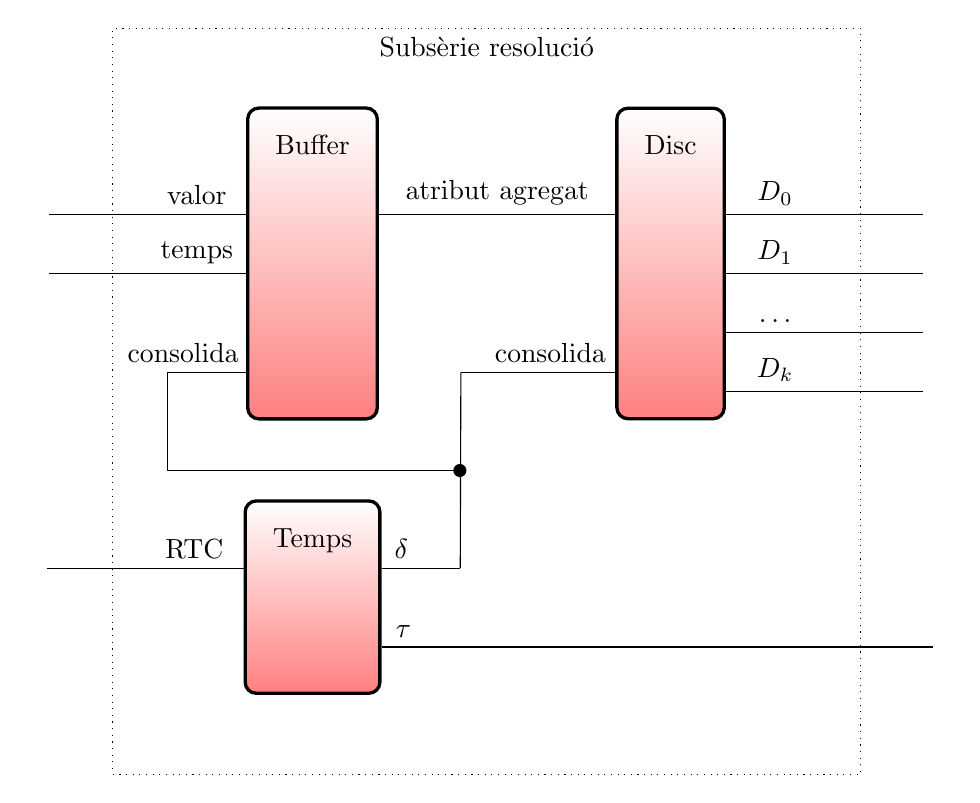
\begin{tikzpicture}
\tikzset{
    maquina/.style={rectangle,rounded corners,draw=black, 
      very thick, inner sep=1em, minimum size=3em, text centered,
      groc},
    interficie/.style={rectangle,rounded corners,draw=black, 
       inner sep=0.2em, minimum size=1em, text centered,
      verd},
    modul/.style={rectangle,rounded corners,draw=black, 
      very thick, inner sep=1em, minimum size=3em, text centered,
      roig},   
    myarrow/.style={->, >=latex', shorten >=1pt, thick},
    fletxaswitch/.style={<->, >=latex',shorten >=10pt,shorten <=10pt, thick},
    mylabel/.style={text width=7em, text centered},
    groc/.style={top color=white, bottom color=yellow!50},
    verd/.style={top color=white, bottom color=green!50},
    roig/.style={top color=white, bottom color=red!50},
  }  

  
   \node (discres) [draw, dotted, minimum width=9.5cm, text depth=9cm, rectangle] {Subsèrie resolució};



  \node[modul,text depth=3cm,below right=1cm and 1.7cm of discres.north west] (buffer) {Buffer};  

  %entrades
  \node[above left=-1.5cm and 2.5cm of buffer.north west] (buffer_valor)   {};
  \draw[-] (buffer_valor) -- (buffer_valor-|buffer.west)
   node[near end,above]{valor};

   \node[below=0.5cm of buffer_valor] (buffer_nou)   {};
   \draw[-] (buffer_nou) -- (buffer_nou-|buffer.west)
   node[near end,above]{temps};

   \node[above left=-3.5cm and 1cm of buffer.north west] (buffer_consolida) {};
   \draw[-] (buffer_consolida) -- (buffer_consolida-|buffer.west)
   node[pos=0.2,above]{consolida};

   %sortides
   \node[above right=-1.5cm and 1.5cm of buffer.north east] (buffer_dada)   {};
  \draw[-] (buffer_dada) -- (buffer_dada-|buffer.east)
   node[pos=0,above]{atribut agregat};





  \node[modul,right=3cm of buffer,text depth=3cm] (disc)   {Disc}; 

  % entrades
  \node[above left=-1.5cm and 2cm of disc.north west] (disc_valor)   {};
  \draw[-] (disc_valor) -- (disc_valor-|disc.west)
   node[near end,above]{};

  \node[above left=-3.5cm and 1.96cm of disc.north west] (disc_consolida)   {};
  \draw[-] (disc_consolida) -- (disc_consolida-|disc.west)
   node[pos=0.58,above]{consolida};

   % sortides
   \node[above right=-1.5cm and 2.5cm of disc.north east] (disc_d0)   {};
   \draw[-] (disc_d0) -- (disc_d0-|disc.east)
   node[near end,above]{$D_0$};

   \node[below=0.5cm of disc_d0] (disc_d1)   {};
  \draw[-] (disc_d1) -- (disc_d1-|disc.east)
   node[near end,above]{$D_1$};

   \node[below=0.5cm of disc_d1] (disc_d2)   {};
  \draw[-] (disc_d2) -- (disc_d2-|disc.east)
   node[near end,above]{$\dots$};

   \node[below=0.5cm of disc_d2] (disc_d3)   {};
  \draw[-] (disc_d3) -- (disc_d3-|disc.east)
   node[near end,above]{$D_k$};




  \node[modul,below=1cm of buffer,text depth=1.5cm] (temps)   {Temps}; 

  % entrades
  \node[above left=-1cm and 2.5cm of temps.north west] (temps_rtc)   {};
  \draw[-] (temps_rtc) -- (temps_rtc-|temps.west)
   node[near end,above]{RTC};

  % sortides
   \node[above right=-1cm and 1cm of temps.north east] (temps_delta)   {};
   \draw[-] (temps_delta) -- (temps_delta-|temps.east)
   node[near end,above]{$\delta$};

   \node[above right=-2cm and 7cm of temps.north east] (temps_tau)   {};
   \draw[-] (temps_tau) -- (temps_tau-|temps.east)
   node[pos=0.96,above]{$\tau$};








   %connexions
   \draw[-] (temps_delta.west) -- (disc_consolida.east); 
   
%   \node[above left=0.3cm and 1cm of temps.north west] (tau_reset)   {};
   \node[below=1cm of buffer_consolida] (tau_reset)   {};
   \draw[-*,shorten >=-2pt] (tau_reset) -- (tau_reset-|disc_consolida.east);
   \draw[-] (tau_reset.east) -- (tau_reset.east|-buffer_consolida);


 \end{tikzpicture}
 
\caption{Esquema genèric d'un disc resolució}
\label{fig:vhdl:disc-resolucio}
\end{figure}


Condicions:
\begin{itemize}
\item Àmbit: xarxes de sensors
\item No apte per processos industrials ni llaços de control, en els
  quals cal tenir totes les dades
\item Possibilitat de validació de dades del sensor (en el buffer) i
  generar avisos de funcionament incorrecte.
\item Interfície per a consulta les dades?
\end{itemize}





Estructures alternatives:
\begin{itemize}
\item timestamps absoluts: $\delta$ creats a partir de RTC
\item timestamps relatius: $\delta$ creats a partir del clock
\item timestamps creixents: l'RTC el marca el temps de la mesura
\item Memòria estàtica en comptes de volàtil. Útil per a: a) tenir dades permanents en cas d'apagada o b) per a poder consumir menys (?)   ->  tot això no seria millor fer-ho per programa (CPU) que implementat físicament (aleshores seria més reprogramable)?
\end{itemize}





Base de dades completa, conjunt de discs resolució:
\usetikzlibrary{shapes,arrows,positioning}

\begin{tikzpicture}
 \tikzset{
        myarrow/.style={->, >=latex',  thick},
      }
      

  \node[rectangle,draw,minimum height=6cm,minimum width=9cm] (m) {};
  \draw[shift=( m.south west)]   
  node[above right] {base de dades multiresolució};


  %discmig
  \node (m.center) (discr1) {...};

  %discr
  
  \node[ellipse,draw,minimum height=3.5cm,minimum width=2.5cm,alias=discr0] [left=of discr1] {};
  \node[above=0cm of discr0.north] {$R_0$};
  \node[below=0cm of discr0] {disc resolució};

  \node[cylinder, draw, shape border rotate=90, aspect=0.25,alias=buffer0] [below=3mm of discr0.north] {buffer};
  \node[circle, draw,alias=disc0]  [above=3mm of discr0.south] {disc} ;
  \draw [->] (disc0.center)++(.4:.4cm) arc(0:180:.4cm);
  \draw[myarrow] (buffer0.bottom) -- (disc0.north);


  %discrd

  \node[ellipse,draw,minimum height=3.5cm,minimum width=2.5cm,alias=discrd] [right=of discr1] {};
  \node[above=0cm of discrd] {$R_d$};
  \node[below=0cm of discrd] {disc resolució};

  \node[cylinder, draw, shape border rotate=90, aspect=0.25,alias=bufferd] [below=3mm of discrd.north] {buffer};
  \node[circle, draw,alias=discd]  [above=3mm of discrd.south] {disc} ;
  \draw [->] (discd.center)++(.4:.4cm) arc(0:180:.4cm);
  \draw[myarrow] (bufferd.bottom) -- (discd.north);



  %mesura 
  \node[above=1cm of m.north] (m0) {};

  \draw[myarrow] (m0) -- (m.north) 
  node[right,midway] {mesura};

  \draw[myarrow] (m.north) -- (buffer0);
  \draw[myarrow] (m.north) -- (bufferd);
  \draw[myarrow] (m.north) -- (discr1);

\end{tikzpicture}




Base de dades amb discs resolució enllaçats:

\begin{tikzpicture}
 \tikzset{
        myarrow/.style={->, >=latex',  thick},
      }
      

  \node[rectangle,draw,minimum height=6cm,minimum width=9cm] (m) {};
  \draw[shift=( m.south west)]   
  node[above right] {base de dades multiresolució};


  %discmig
  \node (m.center) (discr1) {...};

  %discr
  
  \node[ellipse,draw,minimum height=3.5cm,minimum width=2.5cm,alias=discr0] [left=of discr1] {};
  \node[above=0cm of discr0.north] {$R_0$};
  \node[below=0cm of discr0] {disc resolució};

  \node[cylinder, draw, shape border rotate=90, aspect=0.25,alias=buffer0] [below=3mm of discr0.north] {buffer};
  \node[circle, draw,alias=disc0]  [above=3mm of discr0.south] {disc} ;
  \draw [->] (disc0.center)++(.4:.4cm) arc(0:180:.4cm);
  \draw[myarrow] (buffer0.bottom) -- (disc0.north);


  %discrd

  \node[ellipse,draw,minimum height=3.5cm,minimum width=2.5cm,alias=discrd] [right=of discr1] {};
  \node[above=0cm of discrd] {$R_d$};
  \node[below=0cm of discrd] {disc resolució};

  \node[cylinder, draw, shape border rotate=90, aspect=0.25,alias=bufferd] [below=3mm of discrd.north] {buffer};
  \node[circle, draw,alias=discd]  [above=3mm of discrd.south] {disc} ;
  \draw [->] (discd.center)++(.4:.4cm) arc(0:180:.4cm);
  \draw[myarrow] (bufferd.bottom) -- (discd.north);



  %mesura 
  \node[above=1cm of m.north] (m0) {};

  \draw[myarrow] (m0) -- (m.north) 
  node[right,midway] {mesura};

  \draw[myarrow] (m.north) -- (buffer0);
  \draw[myarrow] (discr1.south) -- (bufferd);
  \draw[myarrow] (disc0) -- (discr1.north);

\end{tikzpicture}









% \begin{tikzpicture}[circuit logic IEC,
%   every circuit symbol/.style={
%     logic gate IEC symbol color=black,
%     fill=blue!20,draw=blue,very thick}]
%   \matrix[column sep=7mm]
%   {
%     \node (i0) {0}; &
%     & \\
%     & \node [and gate] (a1) {}; & \\
%     \node (i1) {0}; &
%     & \node [or gate] (o) {};\\
%     & \node [nand gate] (a2) {}; & \\
%     \node (i2) {1}; &
%     & \\
%   };
%   \draw (i0.east) -- ++(right:3mm) |- (a1.input 1);
%   \draw (i1.east) -- ++(right:3mm) |- (a1.input 2);
%   \draw (i1.east) -- ++(right:3mm) |- (a2.input 1);
%   \draw (i2.east) -- ++(right:3mm) |- (a2.input 2);
%   \draw (a1.output) -- ++(right:3mm) |- (o.input 1);
%   \draw (a2.output) -- ++(right:3mm) |- (o.input 2);
%   \draw (o.output) -- ++(right:3mm);
% \end{tikzpicture}








% \def\degr{${}^\circ$}
% \begin{tikztimingtable}
%   Clock 128\,MHz 0\degr    & H   12{2C} G \\ % ends with edge
%   Clock 128\,MHz 90\degr   & [C] 12{2C} C \\ % starts with edge
%   Clock 128\,MHz 180\degr  & C   12{2C} G \\ % ends with edge
%   Clock 128\,MHz 270\degr  &     12{2C} C \\
% \end{tikztimingtable}





\subsection{Possibles aplicacions}

Exemple d'aparell encastat molt petit, per exemple un aparell que
s'hagi de posar dins del cos per a mesurar la temperatura, a on hi ha
molt poc espai disponible i només permet emmagatzemar 100 dades. Es
poden desar 100 valors cada hora = 4 dies, o bé es pot aplicar una
solució de multiresolució i desa 75 valors cada hora = 2 dies i 25
valors cada dia = 25 dies. Així si no s'és a temps de recuperar les
dades en quatre dies sempre hi haurà alguna informació.

Exemple de la implementació de circuits integrats en materials molt prims i doblegables.




Bàsicament en les implementacions a baix nivell d'un SGSTM tenim dues opcions:

\begin{itemize}
\item implementar-ho amb llenguatge de baix nivell (assemblador, C) en un microcontrolador. Aquesta seria la manera típica perquè dóna molta flexibilitat: es pot reconfigurar l'esquema de multiresolució quan es vulgui, es poden utilitzar les operacions que es vulgui, canviar la mida, etc. 

\item implementar-ho amb hardware, per exemple dissenyar amb
  VHDL. Inconvenients: gens flexible (un cop implementat no es pot
  canviar), difícil de fer genèric (no es pot trobar un circuit que
  serveixi per a fer varis càlculs, per això caldria un
  microcontrolador). Avantatges: es pot compactar i encastar en
  llocs petits, estructures de càlcul paral·leles (la feina no recau
  en el microcontrolador), bases de dades distribuïdes. Per tant es fa
  difícil pensar de vendre BDM genèriques hardware però sí que es
  poden pensar algunes possibles aplicacions que només serien
  exclusives de hardware:

  \begin{itemize}
  \item Sensors inte\l.ligents o totalment encastats. Actualment es
    dissenyen sensors acompanyats de circuits digitals, tot encastat
    en un xip petit. Fan filtratge dels senyal, tenen un bus de
    comunicació senzill amb el controlador (I2C, 1-Wire, SPI, etc.), el
    controlador pot indicar quan s'ha d'iniciar la captura d'un no
    valor, s'emmagatzema el darrer valor capturat i el controlador el
    consulta quan vol, poden establir uns llindars d'alarma... Així
    doncs aquests sensors només emmagatzemen el darrer valor, es
    podria proposar que emmagatzemessin amb esquema multiresolució, el
    qual hauria de ser una mica configurable per exemple els períodes
    de consolidació. No obstant això, la configuració seria molt poc
    flexible i si es necessiten càlculs més complicats sempre és
    millor seguir amb l'esquema habitual del microcontrolador captura
    la dada i ell gestiona els càlculs. Ara bé, també es pot entendre
    el sensor inte\l.ligent com que forma part d'una base de dades
    distribuïda i ell té una part de l'emmagatzematge. 
    
  \item Esquema multiresolució encastat en perifèrics per a monitorar
    el seu funcionament: en una impressora en els comptadors
    d'impressions, en una antena de comunicació sense fils en els
    comptadors de bytes transmesos o la potència transmesa, etc.

  \item Implementació de circuits integrats en llocs mai vistos:
    materials molt prims i doblegables. Aquí segurament hi ha
    problemes de la mida dels circuits que es poden implementar, per
    tant poder-hi disposar d'esquemes multiresolució aniria bé.

  \item Possibilitat de disseny de FPGA casolans. Si mai això fos
    possible (sembla que ja és possible: exemple de FPGA a la
    raspberry, System-on-Chip (SoC)), els sensors intel·ligents o
    totalment encastats prendrien molt sentit ja que serien
    reconfigurables o que fos molt barat implementar en hardware un
    circuit i llençar-lo quan es volgués canviar de configuració. Això
    llavors encaixaria amb construir un xip per blocs: hi poso un bloc
    de comunicacions, un bloc de tal i un bloc de base de dades
    multiresolució amb tal esquema. Tot i així, sembla que en els SoC
    la idea és implementar-ho com a microcontrolador i fins i tot
    implementar-hi sistemes operatius.

  \end{itemize}


\end{itemize}

En l'àmbit, no es veu clara la implementació de coses en VHDL. Sembla que es desaprofitar recursos perquè la feina ja la pot fer el microcontrolador. Potser l'aplicació útil i que s'ha de destacar és quan en els xips integrats no hi ha microcontrolador com poder-hi posar una base de dades?


%%% Local Variables:
%%% TeX-master: "main"
%%% End:





%------- Bibliografia ------
\cleardoublepage
%\phantomsection\addcontentsline{toc}{chapter}{\bibname}
\pdfbookmark{\bibname}{bookmark:bibliografia}
\printbibliography
%----------------------------------------------

%\backmatter

\end{document}



%%%%%%%%%%%%%%%%%%%%%%%%%%%%%%%%%%%%%%%%%%%%%%%%%%%%%%%%%%%%%%%%%%%%%%%%%%  
% Memòria Tesi Doctoral. Model d'un sistema de gestió multiresolució per a sèries temporals.
%
% Copyright (C) 2011-2013 Aleix Llusà Serra.
% 
% This LaTeX document is free software: you can redistribute it and/or
% modify it under the terms of the GNU General Public License as
% published by the Free Software Foundation, either version 3 of the
% License, or (at your option) any later version.
%
% This document is distributed in the hope that it will be useful, but
% WITHOUT ANY WARRANTY; without even the implied warranty of
% MERCHANTABILITY or FITNESS FOR A PARTICULAR PURPOSE. See the GNU
% General Public License for more details.
%
% You should have received a copy of the GNU General Public License
% along with this document. If not, see <http://www.gnu.org/licenses/>.
%
%
% Aleix Llusà Serra
% Departament de Disseny i Programació de Sistemes Electrònics de la Universitat Politècnica de Catalunya (DiPSE-UPC)
% Escola Politècnica Superior d'Enginyeria de Manresa (EPSEM)
% Av. de les Bases de Manresa, 61-73
% 08242 Manresa (Barcelona)
% PAÏSOS CATALANS 
%
% aleix (a) dipse.upc.edu
% 
% El codi font LaTeX del document es troba a 
% <http://escriny.epsem.upc.edu/projects/rrb/>
%%%%%%%%%%%%%%%%%%%%%%%%%%%%%%%%%%%%%%%%%%%%%%%%%%%%%%%%%%%%%%%%%%%%%%%%%% 